\documentclass{book}
\usepackage[a4paper,top=2.5cm,bottom=2.5cm,left=2.5cm,right=2.5cm]{geometry}
\usepackage{makeidx}
\usepackage{natbib}
\usepackage{graphicx}
\usepackage{multicol}
\usepackage{float}
\usepackage{listings}
\usepackage{color}
\usepackage{ifthen}
\usepackage[table]{xcolor}
\usepackage{textcomp}
\usepackage{alltt}
\usepackage{ifpdf}
\ifpdf
\usepackage[pdftex,
            pagebackref=true,
            colorlinks=true,
            linkcolor=blue,
            unicode
           ]{hyperref}
\else
\usepackage[ps2pdf,
            pagebackref=true,
            colorlinks=true,
            linkcolor=blue,
            unicode
           ]{hyperref}
\usepackage{pspicture}
\fi
\usepackage[utf8]{inputenc}
\usepackage{mathptmx}
\usepackage[scaled=.90]{helvet}
\usepackage{courier}
\usepackage{sectsty}
\usepackage{amssymb}
\usepackage[titles]{tocloft}
\usepackage{doxygen}
\lstset{language=C++,inputencoding=utf8,basicstyle=\footnotesize,breaklines=true,breakatwhitespace=true,tabsize=8,numbers=left }
\makeindex
\setcounter{tocdepth}{3}
\renewcommand{\footrulewidth}{0.4pt}
\renewcommand{\familydefault}{\sfdefault}
\hfuzz=15pt
\setlength{\emergencystretch}{15pt}
\hbadness=750
\tolerance=750
\begin{document}
\hypersetup{pageanchor=false,citecolor=blue}
\begin{titlepage}
\vspace*{7cm}
\begin{center}
{\Large Phenogene \\[1ex]\large 1.\-0 }\\
\vspace*{1cm}
{\large Generated by Doxygen 1.8.1.2}\\
\vspace*{0.5cm}
{\small Fri Jun 21 2013 15:25:38}\\
\end{center}
\end{titlepage}
\clearemptydoublepage
\pagenumbering{roman}
\tableofcontents
\clearemptydoublepage
\pagenumbering{arabic}
\hypersetup{pageanchor=true,citecolor=blue}
\chapter{Namespace Index}
\section{Namespace List}
Here is a list of all namespaces with brief descriptions\-:\begin{DoxyCompactList}
\item\contentsline{section}{\hyperlink{a00020}{Ui} }{\pageref{db/db2/a00020}}{}
\end{DoxyCompactList}

\chapter{Class Index}
\section{Class List}
Here are the classes, structs, unions and interfaces with brief descriptions\-:\begin{DoxyCompactList}
\item\contentsline{section}{\hyperlink{a00001}{File\-\_\-\-Manager} }{\pageref{d8/d84/a00001}}{}
\item\contentsline{section}{\hyperlink{a00002}{G\-U\-I} }{\pageref{d7/d46/a00002}}{}
\item\contentsline{section}{\hyperlink{a00003}{Neural\-\_\-\-Network} }{\pageref{d1/d7c/a00003}}{}
\end{DoxyCompactList}

\chapter{File Index}
\section{File List}
Here is a list of all files with brief descriptions\-:\begin{DoxyCompactList}
\item\contentsline{section}{phenogene/\hyperlink{a00004}{File\-Manager.\-h} }{\pageref{d0/d0b/a00004}}{}
\item\contentsline{section}{phenogene/\hyperlink{a00005}{F\-M.\-cpp} }{\pageref{dd/dad/a00005}}{}
\item\contentsline{section}{phenogene/\hyperlink{a00006}{F\-M\-\_\-getters.\-cpp} }{\pageref{de/d21/a00006}}{}
\item\contentsline{section}{phenogene/\hyperlink{a00007}{F\-M\-\_\-setters.\-cpp} }{\pageref{de/d5e/a00007}}{}
\item\contentsline{section}{phenogene/\hyperlink{a00008}{General\-\_\-\-Notation.\-h} }{\pageref{d4/dee/a00008}}{}
\item\contentsline{section}{phenogene/\hyperlink{a00009}{G\-U\-I.\-cpp} }{\pageref{da/da0/a00009}}{}
\item\contentsline{section}{phenogene/\hyperlink{a00010}{G\-U\-I.\-h} }{\pageref{d7/dec/a00010}}{}
\item\contentsline{section}{phenogene/\hyperlink{a00011}{G\-U\-I\-\_\-constructor.\-cpp} }{\pageref{da/d45/a00011}}{}
\item\contentsline{section}{phenogene/\hyperlink{a00012}{G\-U\-I\-\_\-start\-Button.\-cpp} }{\pageref{df/d86/a00012}}{}
\item\contentsline{section}{phenogene/\hyperlink{a00013}{main.\-cpp} }{\pageref{d7/dd4/a00013}}{}
\item\contentsline{section}{phenogene/\hyperlink{a00014}{Neural\-Network.\-h} }{\pageref{d2/de7/a00014}}{}
\item\contentsline{section}{phenogene/\hyperlink{a00015}{N\-N.\-cpp} }{\pageref{dd/d1b/a00015}}{}
\item\contentsline{section}{phenogene/\hyperlink{a00016}{N\-N\-\_\-constructor.\-cpp} }{\pageref{d7/d7a/a00016}}{}
\item\contentsline{section}{phenogene/\hyperlink{a00017}{N\-N\-\_\-getters.\-cpp} }{\pageref{d4/d51/a00017}}{}
\item\contentsline{section}{phenogene/\hyperlink{a00018}{N\-N\-\_\-setters.\-cpp} }{\pageref{d1/d2b/a00018}}{}
\end{DoxyCompactList}

\chapter{Namespace Documentation}
\hypertarget{a00020}{\section{Ui Namespace Reference}
\label{db/db2/a00020}\index{Ui@{Ui}}
}

\chapter{Class Documentation}
\hypertarget{a00001}{\section{File\-\_\-\-Manager Class Reference}
\label{d8/d84/a00001}\index{File\-\_\-\-Manager@{File\-\_\-\-Manager}}
}


{\ttfamily \#include $<$File\-Manager.\-h$>$}



Collaboration diagram for File\-\_\-\-Manager\-:\nopagebreak
\begin{figure}[H]
\begin{center}
\leavevmode
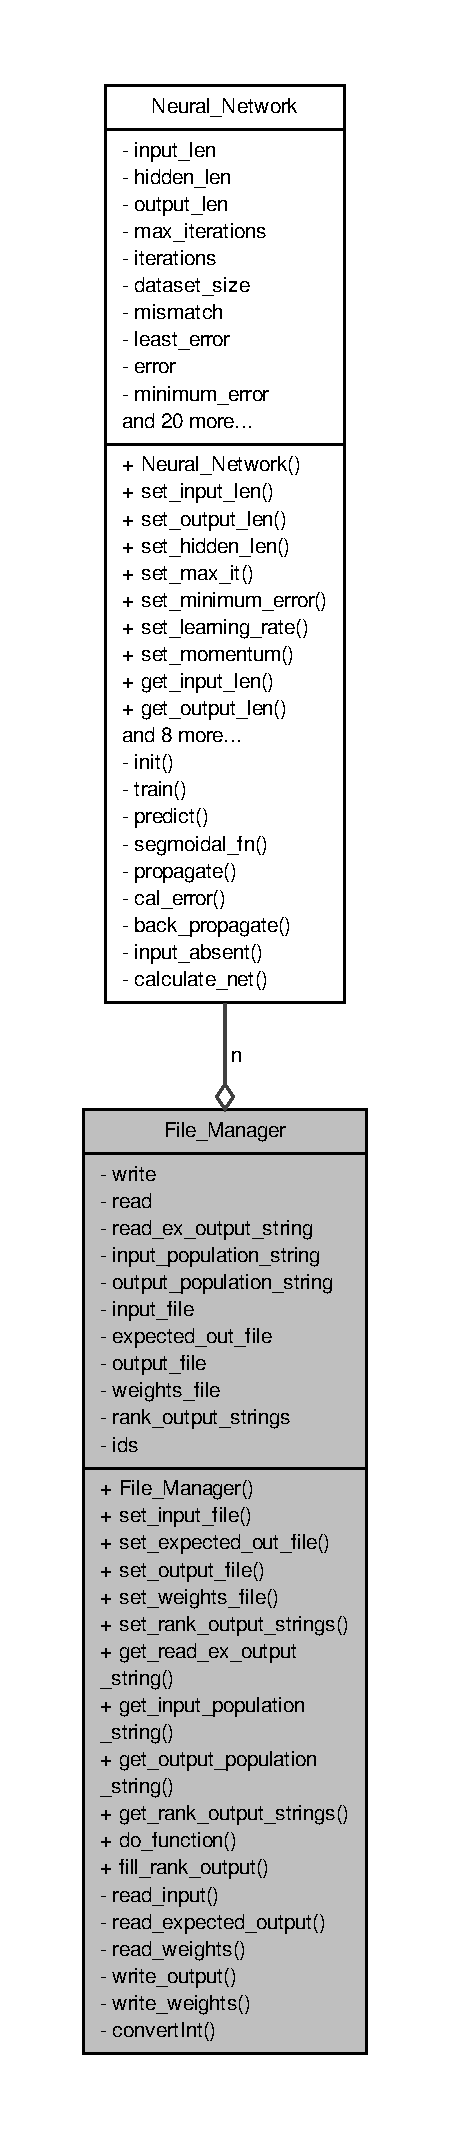
\includegraphics[height=550pt]{d5/db6/a00042}
\end{center}
\end{figure}
\subsection*{Public Member Functions}
\begin{DoxyCompactItemize}
\item 
\hyperlink{a00001_a2acf523335c71f922a42756c1d0a7a2d}{File\-\_\-\-Manager} ()
\item 
void \hyperlink{a00001_af43b27d7ea5f031a20652a43f5b99f53}{set\-\_\-input\-\_\-file} (string)
\begin{DoxyCompactList}\small\item\em Set input file path to string s. \end{DoxyCompactList}\item 
void \hyperlink{a00001_ad83423f6db9466419d4a7acd3e322cb4}{set\-\_\-expected\-\_\-out\-\_\-file} (string)
\begin{DoxyCompactList}\small\item\em Set expected output file path to string s. \end{DoxyCompactList}\item 
void \hyperlink{a00001_a2eff082d4fe4d7f2a7ce06afbc689d45}{set\-\_\-output\-\_\-file} (string)
\begin{DoxyCompactList}\small\item\em Set calculated output file path to string s. \end{DoxyCompactList}\item 
void \hyperlink{a00001_a860e5837e1671018a26fdc0ce43603b1}{set\-\_\-weights\-\_\-file} (string)
\begin{DoxyCompactList}\small\item\em Set weights file path to string s. \end{DoxyCompactList}\item 
void \hyperlink{a00001_af80b18b12b1b619428cf7224cd588594}{set\-\_\-rank\-\_\-output\-\_\-strings} (int, string)
\begin{DoxyCompactList}\small\item\em Set string with index i to s. \end{DoxyCompactList}\item 
string \hyperlink{a00001_ad506966ba52a415b33970c057c9ed43a}{get\-\_\-read\-\_\-ex\-\_\-output\-\_\-string} ()
\begin{DoxyCompactList}\small\item\em Get string expected output content. \end{DoxyCompactList}\item 
string \hyperlink{a00001_a13d1128905d7b4a3bdec2e40392cd036}{get\-\_\-input\-\_\-population\-\_\-string} ()
\begin{DoxyCompactList}\small\item\em Get string input content. \end{DoxyCompactList}\item 
string \hyperlink{a00001_a368e05b24358cc70bd8b7d2081cd0dd4}{get\-\_\-output\-\_\-population\-\_\-string} ()
\begin{DoxyCompactList}\small\item\em Get string output content. \end{DoxyCompactList}\item 
string \hyperlink{a00001_acd21da57c513a63893641ac505c097f0}{get\-\_\-rank\-\_\-output\-\_\-strings} (int)
\begin{DoxyCompactList}\small\item\em Get string represenation for given I\-D. \end{DoxyCompactList}\item 
void \hyperlink{a00001_abcb9cd1427a3b6ecfd41432391ec9bdc}{do\-\_\-function} (int)
\begin{DoxyCompactList}\small\item\em Call rotine specified by parameter mode. \end{DoxyCompactList}\item 
void \hyperlink{a00001_a44a6161fabb28c07ba6e860ba9927aa6}{fill\-\_\-rank\-\_\-output} ()
\begin{DoxyCompactList}\small\item\em Interface to fill the output/decimal association\par
 associates each output node with a string. \end{DoxyCompactList}\end{DoxyCompactItemize}
\subsection*{Public Attributes}
\begin{DoxyCompactItemize}
\item 
\hyperlink{a00003}{Neural\-\_\-\-Network} \hyperlink{a00001_ac70ea2427e95618bb3903b2c57ee9745}{n}
\end{DoxyCompactItemize}
\subsection*{Private Member Functions}
\begin{DoxyCompactItemize}
\item 
void \hyperlink{a00001_a1134b607af353e187667aaba1a960bdd}{read\-\_\-input} (string)
\begin{DoxyCompactList}\small\item\em Opens file file\-Path and reads its content. \end{DoxyCompactList}\item 
void \hyperlink{a00001_a4b0a0ad74a4446e5f23020521200b932}{read\-\_\-expected\-\_\-output} (string)
\begin{DoxyCompactList}\small\item\em Read expected output\par
 Opens file file\-Path and reads its content. \end{DoxyCompactList}\item 
void \hyperlink{a00001_a7d2759b2ad892445e7d74892737547cf}{read\-\_\-weights} (string)
\begin{DoxyCompactList}\small\item\em Read weights for hidden and output layer.\par
 Opens file file\-Path and reads its content. \end{DoxyCompactList}\item 
void \hyperlink{a00001_a4e104949ad8e8fd75c612313f857ee5a}{write\-\_\-output} (string)
\begin{DoxyCompactList}\small\item\em Write output\par
 Opens file file\-Path and write to it. \end{DoxyCompactList}\item 
void \hyperlink{a00001_a67e37c5e1429df91a8c4ff836579cdc0}{write\-\_\-weights} (string)
\begin{DoxyCompactList}\small\item\em Write weights\par
 Opens file file\-Path and write to it. \end{DoxyCompactList}\item 
string \hyperlink{a00001_a6b29a9f88396627c1d39170723bad7fd}{convert\-Int} (int)
\begin{DoxyCompactList}\small\item\em Converts integer number to string. \end{DoxyCompactList}\end{DoxyCompactItemize}
\subsection*{Private Attributes}
\begin{DoxyCompactItemize}
\item 
ofstream \hyperlink{a00001_a7d29cb8d04a1a60638f653c28a628095}{write}
\item 
ifstream \hyperlink{a00001_a035fb2bdf99f8f928d049bc950c81f4c}{read}
\item 
string \hyperlink{a00001_af7d8ea2c0a997e16600478c0020b1858}{read\-\_\-ex\-\_\-output\-\_\-string}
\item 
string \hyperlink{a00001_a80f6d8f738cbc4d10154b470c5422fdd}{input\-\_\-population\-\_\-string}
\item 
string \hyperlink{a00001_a4266a9bec2fff5d17d7abf06e00384db}{output\-\_\-population\-\_\-string}
\item 
string \hyperlink{a00001_a78b144182e3cfc70f9aae78ebdd66e51}{input\-\_\-file}
\item 
string \hyperlink{a00001_a8b8f5c9cc3ffcb083ccc4fce1c05ca44}{expected\-\_\-out\-\_\-file}
\item 
string \hyperlink{a00001_a63725670a06637b4290c54eba671b640}{output\-\_\-file}
\item 
string \hyperlink{a00001_aab02256124e6eb39e10e3c9765f0bcb3}{weights\-\_\-file}
\item 
string \hyperlink{a00001_a578abb99a35121fea6c83f1dc21cc2af}{rank\-\_\-output\-\_\-strings} \mbox{[}\hyperlink{a00008_a0a0ddfc9fb3bc3d90d175ed1f7bd54c5}{output\-\_\-l}\mbox{]}
\end{DoxyCompactItemize}


\subsection{Detailed Description}


Definition at line 7 of file File\-Manager.\-h.



\subsection{Constructor \& Destructor Documentation}
\hypertarget{a00001_a2acf523335c71f922a42756c1d0a7a2d}{\index{File\-\_\-\-Manager@{File\-\_\-\-Manager}!File\-\_\-\-Manager@{File\-\_\-\-Manager}}
\index{File\-\_\-\-Manager@{File\-\_\-\-Manager}!File_Manager@{File\-\_\-\-Manager}}
\subsubsection[{File\-\_\-\-Manager}]{\setlength{\rightskip}{0pt plus 5cm}File\-\_\-\-Manager\-::\-File\-\_\-\-Manager (
\begin{DoxyParamCaption}
{}
\end{DoxyParamCaption}
)}}\label{d8/d84/a00001_a2acf523335c71f922a42756c1d0a7a2d}


Definition at line 3 of file F\-M.\-cpp.



\subsection{Member Function Documentation}
\hypertarget{a00001_a6b29a9f88396627c1d39170723bad7fd}{\index{File\-\_\-\-Manager@{File\-\_\-\-Manager}!convert\-Int@{convert\-Int}}
\index{convert\-Int@{convert\-Int}!File_Manager@{File\-\_\-\-Manager}}
\subsubsection[{convert\-Int}]{\setlength{\rightskip}{0pt plus 5cm}string File\-\_\-\-Manager\-::convert\-Int (
\begin{DoxyParamCaption}
\item[{int}]{number}
\end{DoxyParamCaption}
)\hspace{0.3cm}{\ttfamily [private]}}}\label{d8/d84/a00001_a6b29a9f88396627c1d39170723bad7fd}


Converts integer number to string. 


\begin{DoxyParams}{Parameters}
{\em \mbox{[}number\mbox{]}} & Integer to be converted. \\
\hline
\end{DoxyParams}
\begin{DoxyReturn}{Returns}
Number in string format. 
\end{DoxyReturn}


Definition at line 199 of file F\-M.\-cpp.



Here is the caller graph for this function\-:\nopagebreak
\begin{figure}[H]
\begin{center}
\leavevmode
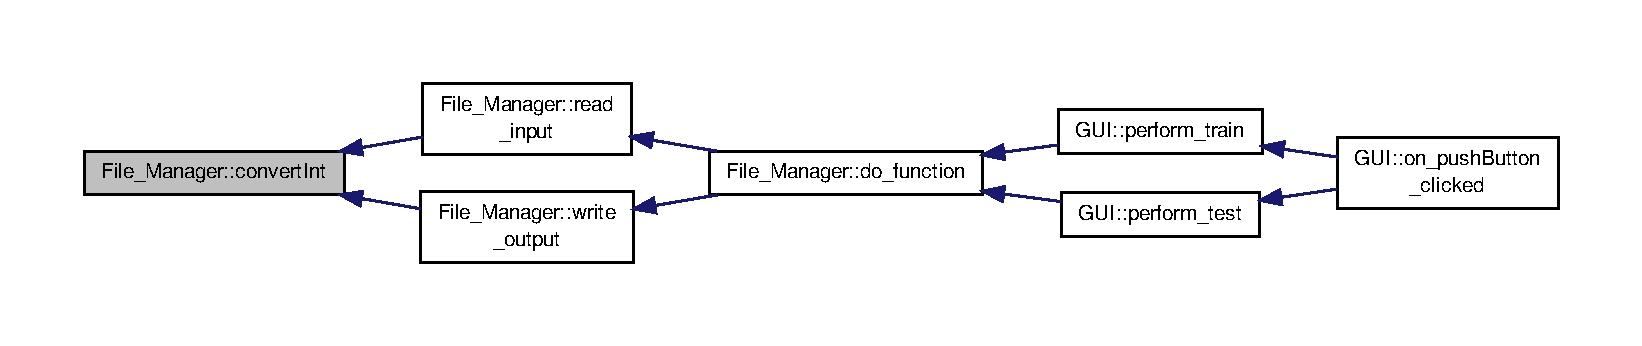
\includegraphics[width=350pt]{d8/d84/a00001_a6b29a9f88396627c1d39170723bad7fd_icgraph}
\end{center}
\end{figure}


\hypertarget{a00001_abcb9cd1427a3b6ecfd41432391ec9bdc}{\index{File\-\_\-\-Manager@{File\-\_\-\-Manager}!do\-\_\-function@{do\-\_\-function}}
\index{do\-\_\-function@{do\-\_\-function}!File_Manager@{File\-\_\-\-Manager}}
\subsubsection[{do\-\_\-function}]{\setlength{\rightskip}{0pt plus 5cm}void File\-\_\-\-Manager\-::do\-\_\-function (
\begin{DoxyParamCaption}
\item[{int}]{mode}
\end{DoxyParamCaption}
)}}\label{d8/d84/a00001_abcb9cd1427a3b6ecfd41432391ec9bdc}


Call rotine specified by parameter mode. 


\begin{DoxyParams}{Parameters}
{\em \mbox{[}mode\mbox{]}} & mode = 1\-: read from input file\par
 mode = 2\-: write to output file\par
 mode = 3\-: read from weights file\par
 mode = 4\-: write to weights file\par
 \\
\hline
\end{DoxyParams}


Definition at line 15 of file F\-M.\-cpp.



References expected\-\_\-out\-\_\-file, input\-\_\-file, output\-\_\-file, read\-\_\-expected\-\_\-output(), read\-\_\-input(), read\-\_\-weights(), weights\-\_\-file, write\-\_\-output(), and write\-\_\-weights().



Here is the call graph for this function\-:\nopagebreak
\begin{figure}[H]
\begin{center}
\leavevmode
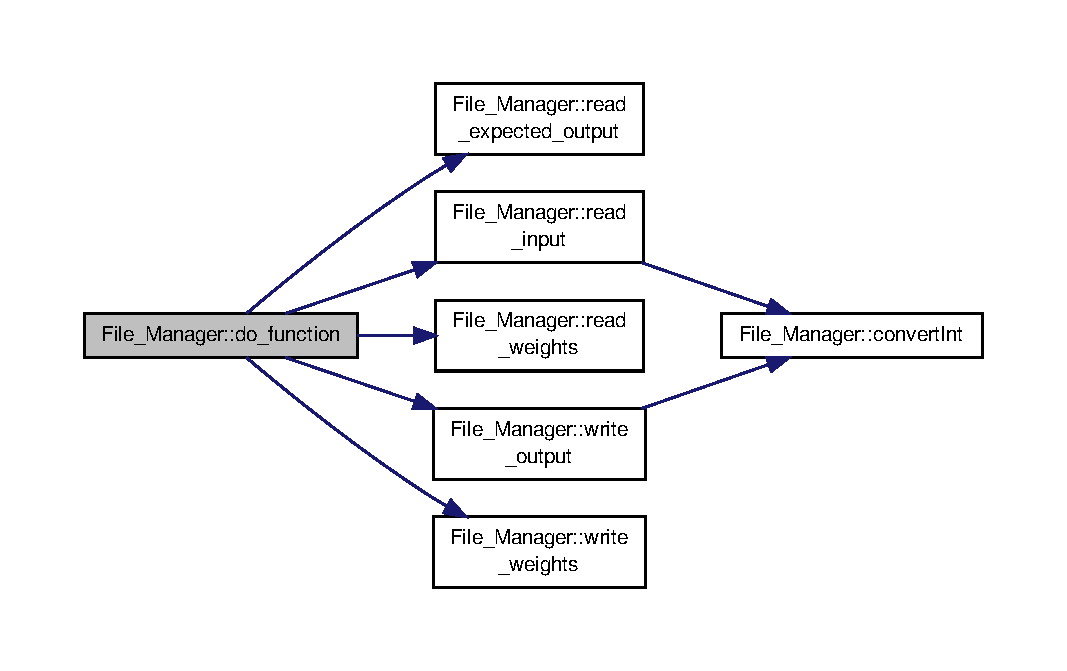
\includegraphics[width=350pt]{d8/d84/a00001_abcb9cd1427a3b6ecfd41432391ec9bdc_cgraph}
\end{center}
\end{figure}




Here is the caller graph for this function\-:\nopagebreak
\begin{figure}[H]
\begin{center}
\leavevmode
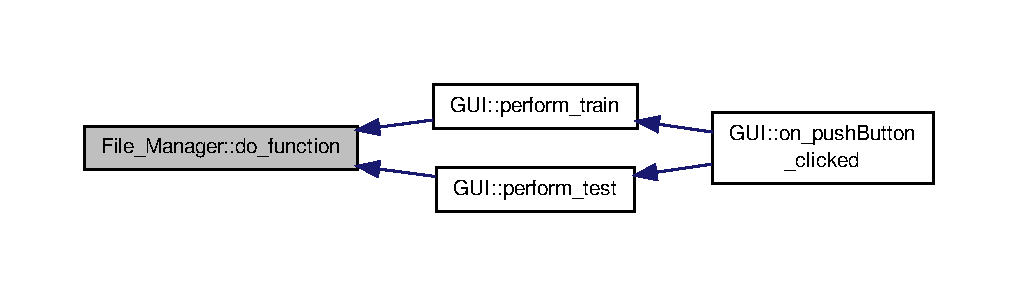
\includegraphics[width=350pt]{d8/d84/a00001_abcb9cd1427a3b6ecfd41432391ec9bdc_icgraph}
\end{center}
\end{figure}


\hypertarget{a00001_a44a6161fabb28c07ba6e860ba9927aa6}{\index{File\-\_\-\-Manager@{File\-\_\-\-Manager}!fill\-\_\-rank\-\_\-output@{fill\-\_\-rank\-\_\-output}}
\index{fill\-\_\-rank\-\_\-output@{fill\-\_\-rank\-\_\-output}!File_Manager@{File\-\_\-\-Manager}}
\subsubsection[{fill\-\_\-rank\-\_\-output}]{\setlength{\rightskip}{0pt plus 5cm}void File\-\_\-\-Manager\-::fill\-\_\-rank\-\_\-output (
\begin{DoxyParamCaption}
{}
\end{DoxyParamCaption}
)}}\label{d8/d84/a00001_a44a6161fabb28c07ba6e860ba9927aa6}


Interface to fill the output/decimal association\par
 associates each output node with a string. 

\begin{DoxyPostcond}{Postcondition}
Output\-\_\-rank is filled. 

Rank\-\_\-output is filled. 
\end{DoxyPostcond}


Definition at line 221 of file F\-M.\-cpp.



References fori, n, Neural\-\_\-\-Network\-::output\-\_\-len, Neural\-\_\-\-Network\-::output\-\_\-rank, Neural\-\_\-\-Network\-::rank\-\_\-output, and rank\-\_\-output\-\_\-strings.



Here is the caller graph for this function\-:\nopagebreak
\begin{figure}[H]
\begin{center}
\leavevmode
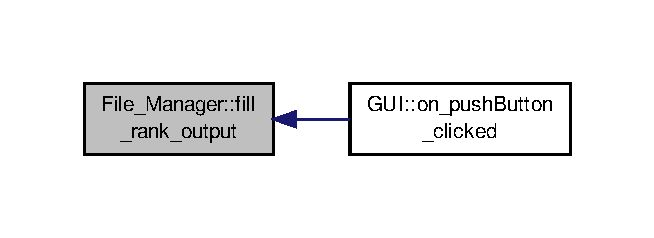
\includegraphics[width=314pt]{d8/d84/a00001_a44a6161fabb28c07ba6e860ba9927aa6_icgraph}
\end{center}
\end{figure}


\hypertarget{a00001_a13d1128905d7b4a3bdec2e40392cd036}{\index{File\-\_\-\-Manager@{File\-\_\-\-Manager}!get\-\_\-input\-\_\-population\-\_\-string@{get\-\_\-input\-\_\-population\-\_\-string}}
\index{get\-\_\-input\-\_\-population\-\_\-string@{get\-\_\-input\-\_\-population\-\_\-string}!File_Manager@{File\-\_\-\-Manager}}
\subsubsection[{get\-\_\-input\-\_\-population\-\_\-string}]{\setlength{\rightskip}{0pt plus 5cm}string File\-\_\-\-Manager\-::get\-\_\-input\-\_\-population\-\_\-string (
\begin{DoxyParamCaption}
{}
\end{DoxyParamCaption}
)}}\label{d8/d84/a00001_a13d1128905d7b4a3bdec2e40392cd036}


Get string input content. 



Definition at line 13 of file F\-M\-\_\-getters.\-cpp.



References input\-\_\-population\-\_\-string.



Here is the caller graph for this function\-:\nopagebreak
\begin{figure}[H]
\begin{center}
\leavevmode
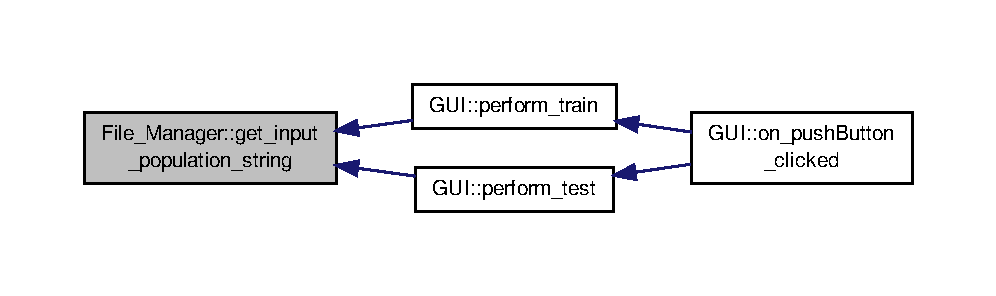
\includegraphics[width=350pt]{d8/d84/a00001_a13d1128905d7b4a3bdec2e40392cd036_icgraph}
\end{center}
\end{figure}


\hypertarget{a00001_a368e05b24358cc70bd8b7d2081cd0dd4}{\index{File\-\_\-\-Manager@{File\-\_\-\-Manager}!get\-\_\-output\-\_\-population\-\_\-string@{get\-\_\-output\-\_\-population\-\_\-string}}
\index{get\-\_\-output\-\_\-population\-\_\-string@{get\-\_\-output\-\_\-population\-\_\-string}!File_Manager@{File\-\_\-\-Manager}}
\subsubsection[{get\-\_\-output\-\_\-population\-\_\-string}]{\setlength{\rightskip}{0pt plus 5cm}string File\-\_\-\-Manager\-::get\-\_\-output\-\_\-population\-\_\-string (
\begin{DoxyParamCaption}
{}
\end{DoxyParamCaption}
)}}\label{d8/d84/a00001_a368e05b24358cc70bd8b7d2081cd0dd4}


Get string output content. 



Definition at line 20 of file F\-M\-\_\-getters.\-cpp.



References output\-\_\-population\-\_\-string.



Here is the caller graph for this function\-:\nopagebreak
\begin{figure}[H]
\begin{center}
\leavevmode
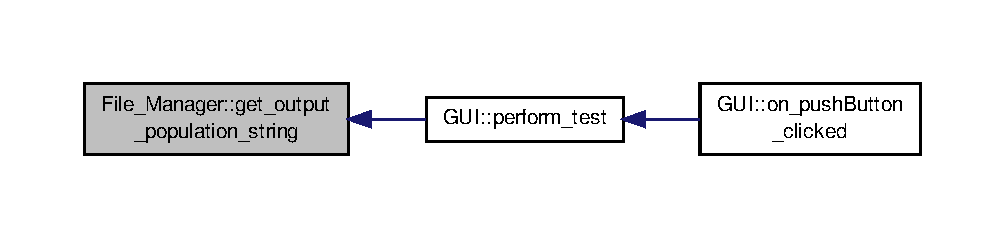
\includegraphics[width=350pt]{d8/d84/a00001_a368e05b24358cc70bd8b7d2081cd0dd4_icgraph}
\end{center}
\end{figure}


\hypertarget{a00001_acd21da57c513a63893641ac505c097f0}{\index{File\-\_\-\-Manager@{File\-\_\-\-Manager}!get\-\_\-rank\-\_\-output\-\_\-strings@{get\-\_\-rank\-\_\-output\-\_\-strings}}
\index{get\-\_\-rank\-\_\-output\-\_\-strings@{get\-\_\-rank\-\_\-output\-\_\-strings}!File_Manager@{File\-\_\-\-Manager}}
\subsubsection[{get\-\_\-rank\-\_\-output\-\_\-strings}]{\setlength{\rightskip}{0pt plus 5cm}string File\-\_\-\-Manager\-::get\-\_\-rank\-\_\-output\-\_\-strings (
\begin{DoxyParamCaption}
\item[{int}]{i}
\end{DoxyParamCaption}
)}}\label{d8/d84/a00001_acd21da57c513a63893641ac505c097f0}


Get string represenation for given I\-D. 



Definition at line 27 of file F\-M\-\_\-getters.\-cpp.



References rank\-\_\-output\-\_\-strings.



Here is the caller graph for this function\-:\nopagebreak
\begin{figure}[H]
\begin{center}
\leavevmode
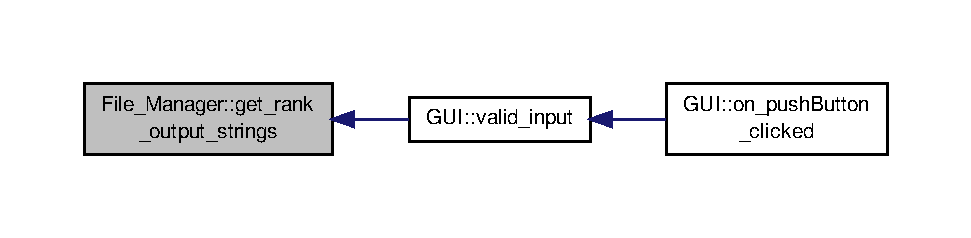
\includegraphics[width=350pt]{d8/d84/a00001_acd21da57c513a63893641ac505c097f0_icgraph}
\end{center}
\end{figure}


\hypertarget{a00001_ad506966ba52a415b33970c057c9ed43a}{\index{File\-\_\-\-Manager@{File\-\_\-\-Manager}!get\-\_\-read\-\_\-ex\-\_\-output\-\_\-string@{get\-\_\-read\-\_\-ex\-\_\-output\-\_\-string}}
\index{get\-\_\-read\-\_\-ex\-\_\-output\-\_\-string@{get\-\_\-read\-\_\-ex\-\_\-output\-\_\-string}!File_Manager@{File\-\_\-\-Manager}}
\subsubsection[{get\-\_\-read\-\_\-ex\-\_\-output\-\_\-string}]{\setlength{\rightskip}{0pt plus 5cm}string File\-\_\-\-Manager\-::get\-\_\-read\-\_\-ex\-\_\-output\-\_\-string (
\begin{DoxyParamCaption}
{}
\end{DoxyParamCaption}
)}}\label{d8/d84/a00001_ad506966ba52a415b33970c057c9ed43a}


Get string expected output content. 



Definition at line 6 of file F\-M\-\_\-getters.\-cpp.



References read\-\_\-ex\-\_\-output\-\_\-string.



Here is the caller graph for this function\-:\nopagebreak
\begin{figure}[H]
\begin{center}
\leavevmode
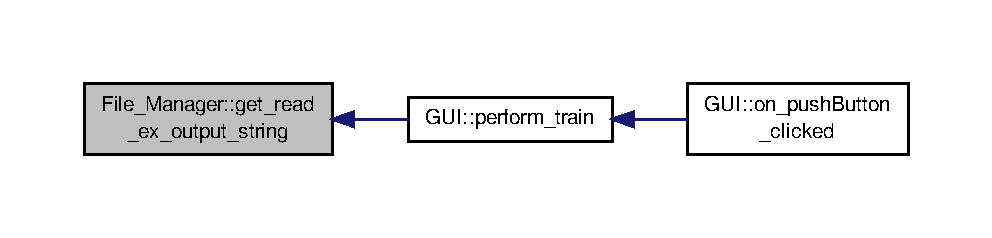
\includegraphics[width=350pt]{d8/d84/a00001_ad506966ba52a415b33970c057c9ed43a_icgraph}
\end{center}
\end{figure}


\hypertarget{a00001_a4b0a0ad74a4446e5f23020521200b932}{\index{File\-\_\-\-Manager@{File\-\_\-\-Manager}!read\-\_\-expected\-\_\-output@{read\-\_\-expected\-\_\-output}}
\index{read\-\_\-expected\-\_\-output@{read\-\_\-expected\-\_\-output}!File_Manager@{File\-\_\-\-Manager}}
\subsubsection[{read\-\_\-expected\-\_\-output}]{\setlength{\rightskip}{0pt plus 5cm}void File\-\_\-\-Manager\-::read\-\_\-expected\-\_\-output (
\begin{DoxyParamCaption}
\item[{string}]{file\-Path}
\end{DoxyParamCaption}
)\hspace{0.3cm}{\ttfamily [private]}}}\label{d8/d84/a00001_a4b0a0ad74a4446e5f23020521200b932}


Read expected output\par
 Opens file file\-Path and reads its content. 


\begin{DoxyParams}{Parameters}
{\em \mbox{[}file\-Path\mbox{]}} & File path to be read. \\
\hline
\end{DoxyParams}
\begin{DoxyPrecond}{Precondition}
File specified by file\-Path is in the correct format. 
\end{DoxyPrecond}
\begin{DoxyPostcond}{Postcondition}
Expected output dataset is filled. 
\end{DoxyPostcond}


Definition at line 91 of file F\-M.\-cpp.



References Neural\-\_\-\-Network\-::dataset\-\_\-size, Neural\-\_\-\-Network\-::expected\-\_\-o, fori, forj, max\-\_\-dataset\-\_\-size, n, Neural\-\_\-\-Network\-::output\-\_\-dataset, Neural\-\_\-\-Network\-::output\-\_\-len, Neural\-\_\-\-Network\-::output\-\_\-rank, read, and read\-\_\-ex\-\_\-output\-\_\-string.



Here is the caller graph for this function\-:\nopagebreak
\begin{figure}[H]
\begin{center}
\leavevmode
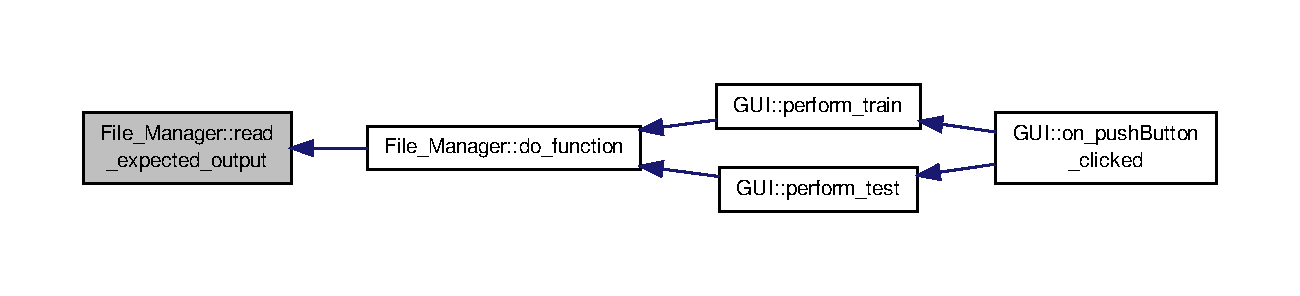
\includegraphics[width=350pt]{d8/d84/a00001_a4b0a0ad74a4446e5f23020521200b932_icgraph}
\end{center}
\end{figure}


\hypertarget{a00001_a1134b607af353e187667aaba1a960bdd}{\index{File\-\_\-\-Manager@{File\-\_\-\-Manager}!read\-\_\-input@{read\-\_\-input}}
\index{read\-\_\-input@{read\-\_\-input}!File_Manager@{File\-\_\-\-Manager}}
\subsubsection[{read\-\_\-input}]{\setlength{\rightskip}{0pt plus 5cm}void File\-\_\-\-Manager\-::read\-\_\-input (
\begin{DoxyParamCaption}
\item[{string}]{file\-Path}
\end{DoxyParamCaption}
)\hspace{0.3cm}{\ttfamily [private]}}}\label{d8/d84/a00001_a1134b607af353e187667aaba1a960bdd}


Opens file file\-Path and reads its content. 

$\ast$\-Read input 
\begin{DoxyParams}{Parameters}
{\em \mbox{[}file\-Path\mbox{]}} & File path to be read. \\
\hline
\end{DoxyParams}
\begin{DoxyPrecond}{Precondition}
File specified by file\-Path is in the correct format. 
\end{DoxyPrecond}
\begin{DoxyPostcond}{Postcondition}
Input dataset is filled. 
\end{DoxyPostcond}


Definition at line 46 of file F\-M.\-cpp.



References convert\-Int(), Neural\-\_\-\-Network\-::dataset\-\_\-size, fori, fork, Neural\-\_\-\-Network\-::input, Neural\-\_\-\-Network\-::input\-\_\-dataset, Neural\-\_\-\-Network\-::input\-\_\-len, input\-\_\-population\-\_\-string, Neural\-\_\-\-Network\-::input\-\_\-rank, max\-\_\-dataset\-\_\-size, n, and read.



Here is the call graph for this function\-:\nopagebreak
\begin{figure}[H]
\begin{center}
\leavevmode
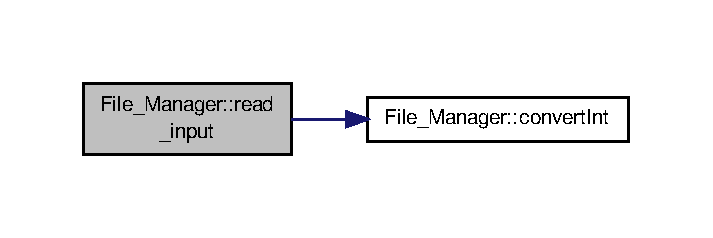
\includegraphics[width=342pt]{d8/d84/a00001_a1134b607af353e187667aaba1a960bdd_cgraph}
\end{center}
\end{figure}




Here is the caller graph for this function\-:\nopagebreak
\begin{figure}[H]
\begin{center}
\leavevmode
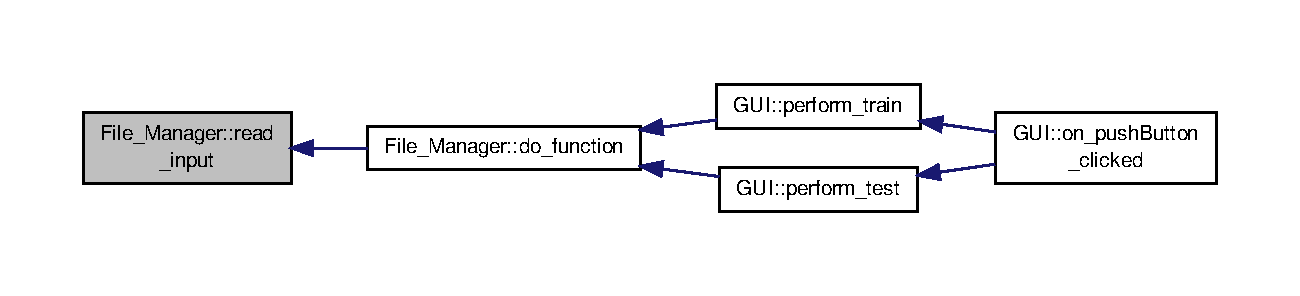
\includegraphics[width=350pt]{d8/d84/a00001_a1134b607af353e187667aaba1a960bdd_icgraph}
\end{center}
\end{figure}


\hypertarget{a00001_a7d2759b2ad892445e7d74892737547cf}{\index{File\-\_\-\-Manager@{File\-\_\-\-Manager}!read\-\_\-weights@{read\-\_\-weights}}
\index{read\-\_\-weights@{read\-\_\-weights}!File_Manager@{File\-\_\-\-Manager}}
\subsubsection[{read\-\_\-weights}]{\setlength{\rightskip}{0pt plus 5cm}void File\-\_\-\-Manager\-::read\-\_\-weights (
\begin{DoxyParamCaption}
\item[{string}]{file\-Path}
\end{DoxyParamCaption}
)\hspace{0.3cm}{\ttfamily [private]}}}\label{d8/d84/a00001_a7d2759b2ad892445e7d74892737547cf}


Read weights for hidden and output layer.\par
 Opens file file\-Path and reads its content. 


\begin{DoxyParams}{Parameters}
{\em \mbox{[}file\-Path\mbox{]}} & File path to be read. \\
\hline
\end{DoxyParams}
\begin{DoxyPrecond}{Precondition}
File specified by file\-Path is in the correct format. 
\end{DoxyPrecond}
\begin{DoxyPostcond}{Postcondition}
Weights datasets are filled. 
\end{DoxyPostcond}


Definition at line 160 of file F\-M.\-cpp.



References fori, forj, Neural\-\_\-\-Network\-::hidden\-\_\-len, Neural\-\_\-\-Network\-::input\-\_\-len, n, Neural\-\_\-\-Network\-::output\-\_\-len, read, Neural\-\_\-\-Network\-::\-Wh, and Neural\-\_\-\-Network\-::\-Wo.



Here is the caller graph for this function\-:\nopagebreak
\begin{figure}[H]
\begin{center}
\leavevmode
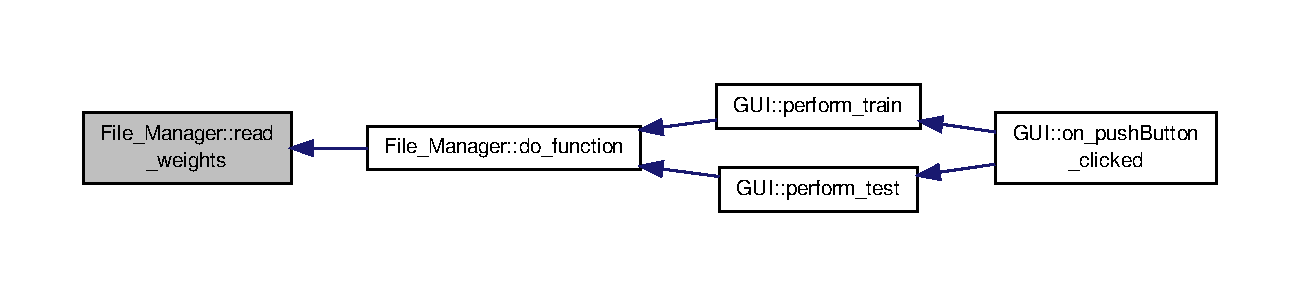
\includegraphics[width=350pt]{d8/d84/a00001_a7d2759b2ad892445e7d74892737547cf_icgraph}
\end{center}
\end{figure}


\hypertarget{a00001_ad83423f6db9466419d4a7acd3e322cb4}{\index{File\-\_\-\-Manager@{File\-\_\-\-Manager}!set\-\_\-expected\-\_\-out\-\_\-file@{set\-\_\-expected\-\_\-out\-\_\-file}}
\index{set\-\_\-expected\-\_\-out\-\_\-file@{set\-\_\-expected\-\_\-out\-\_\-file}!File_Manager@{File\-\_\-\-Manager}}
\subsubsection[{set\-\_\-expected\-\_\-out\-\_\-file}]{\setlength{\rightskip}{0pt plus 5cm}void File\-\_\-\-Manager\-::set\-\_\-expected\-\_\-out\-\_\-file (
\begin{DoxyParamCaption}
\item[{string}]{s}
\end{DoxyParamCaption}
)}}\label{d8/d84/a00001_ad83423f6db9466419d4a7acd3e322cb4}


Set expected output file path to string s. 


\begin{DoxyParams}{Parameters}
{\em \mbox{[}string} & s\mbox{]} expected output file path \\
\hline
\end{DoxyParams}


Definition at line 16 of file F\-M\-\_\-setters.\-cpp.



References expected\-\_\-out\-\_\-file.



Here is the caller graph for this function\-:\nopagebreak
\begin{figure}[H]
\begin{center}
\leavevmode
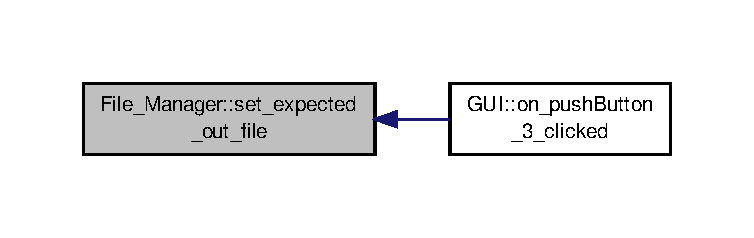
\includegraphics[width=350pt]{d8/d84/a00001_ad83423f6db9466419d4a7acd3e322cb4_icgraph}
\end{center}
\end{figure}


\hypertarget{a00001_af43b27d7ea5f031a20652a43f5b99f53}{\index{File\-\_\-\-Manager@{File\-\_\-\-Manager}!set\-\_\-input\-\_\-file@{set\-\_\-input\-\_\-file}}
\index{set\-\_\-input\-\_\-file@{set\-\_\-input\-\_\-file}!File_Manager@{File\-\_\-\-Manager}}
\subsubsection[{set\-\_\-input\-\_\-file}]{\setlength{\rightskip}{0pt plus 5cm}void File\-\_\-\-Manager\-::set\-\_\-input\-\_\-file (
\begin{DoxyParamCaption}
\item[{string}]{s}
\end{DoxyParamCaption}
)}}\label{d8/d84/a00001_af43b27d7ea5f031a20652a43f5b99f53}


Set input file path to string s. 


\begin{DoxyParams}{Parameters}
{\em \mbox{[}string} & s\mbox{]} input file path \\
\hline
\end{DoxyParams}


Definition at line 7 of file F\-M\-\_\-setters.\-cpp.



References input\-\_\-file.



Here is the caller graph for this function\-:\nopagebreak
\begin{figure}[H]
\begin{center}
\leavevmode
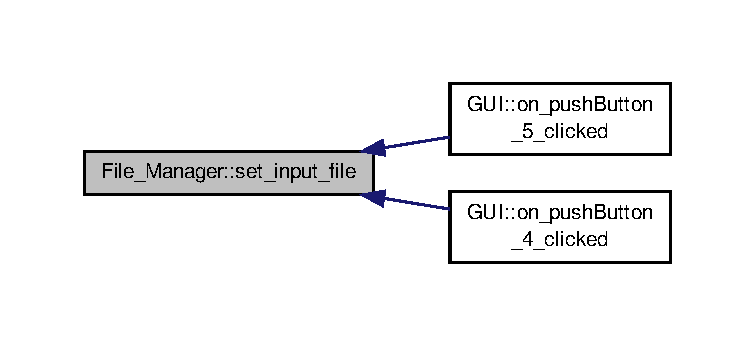
\includegraphics[width=350pt]{d8/d84/a00001_af43b27d7ea5f031a20652a43f5b99f53_icgraph}
\end{center}
\end{figure}


\hypertarget{a00001_a2eff082d4fe4d7f2a7ce06afbc689d45}{\index{File\-\_\-\-Manager@{File\-\_\-\-Manager}!set\-\_\-output\-\_\-file@{set\-\_\-output\-\_\-file}}
\index{set\-\_\-output\-\_\-file@{set\-\_\-output\-\_\-file}!File_Manager@{File\-\_\-\-Manager}}
\subsubsection[{set\-\_\-output\-\_\-file}]{\setlength{\rightskip}{0pt plus 5cm}void File\-\_\-\-Manager\-::set\-\_\-output\-\_\-file (
\begin{DoxyParamCaption}
\item[{string}]{s}
\end{DoxyParamCaption}
)}}\label{d8/d84/a00001_a2eff082d4fe4d7f2a7ce06afbc689d45}


Set calculated output file path to string s. 


\begin{DoxyParams}{Parameters}
{\em \mbox{[}string} & s\mbox{]} output file path \\
\hline
\end{DoxyParams}


Definition at line 25 of file F\-M\-\_\-setters.\-cpp.



References output\-\_\-file.



Here is the caller graph for this function\-:\nopagebreak
\begin{figure}[H]
\begin{center}
\leavevmode
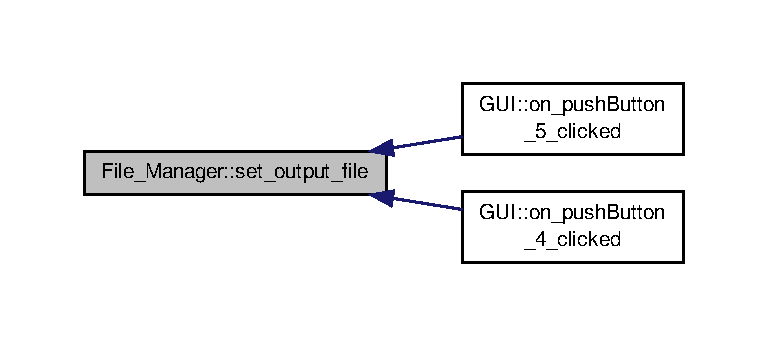
\includegraphics[width=350pt]{d8/d84/a00001_a2eff082d4fe4d7f2a7ce06afbc689d45_icgraph}
\end{center}
\end{figure}


\hypertarget{a00001_af80b18b12b1b619428cf7224cd588594}{\index{File\-\_\-\-Manager@{File\-\_\-\-Manager}!set\-\_\-rank\-\_\-output\-\_\-strings@{set\-\_\-rank\-\_\-output\-\_\-strings}}
\index{set\-\_\-rank\-\_\-output\-\_\-strings@{set\-\_\-rank\-\_\-output\-\_\-strings}!File_Manager@{File\-\_\-\-Manager}}
\subsubsection[{set\-\_\-rank\-\_\-output\-\_\-strings}]{\setlength{\rightskip}{0pt plus 5cm}void File\-\_\-\-Manager\-::set\-\_\-rank\-\_\-output\-\_\-strings (
\begin{DoxyParamCaption}
\item[{int}]{i, }
\item[{string}]{s}
\end{DoxyParamCaption}
)}}\label{d8/d84/a00001_af80b18b12b1b619428cf7224cd588594}


Set string with index i to s. 


\begin{DoxyParams}{Parameters}
{\em \mbox{[}int} & i\mbox{]} Index i of rank\-\_\-output\-\_\-strings \\
\hline
{\em \mbox{[}string} & s\mbox{]} Output keyword \\
\hline
\end{DoxyParams}


Definition at line 45 of file F\-M\-\_\-setters.\-cpp.



References rank\-\_\-output\-\_\-strings.



Here is the caller graph for this function\-:\nopagebreak
\begin{figure}[H]
\begin{center}
\leavevmode
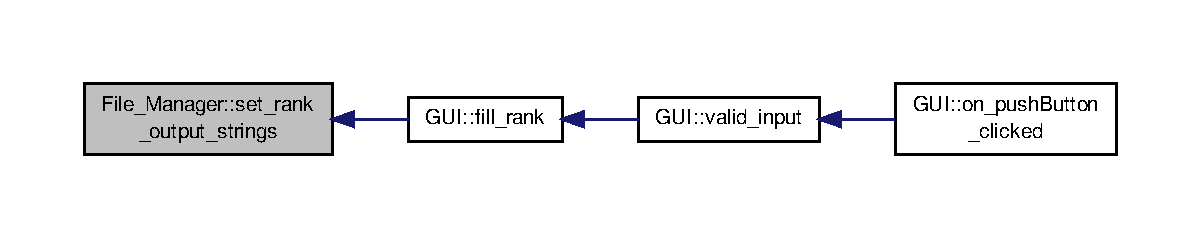
\includegraphics[width=350pt]{d8/d84/a00001_af80b18b12b1b619428cf7224cd588594_icgraph}
\end{center}
\end{figure}


\hypertarget{a00001_a860e5837e1671018a26fdc0ce43603b1}{\index{File\-\_\-\-Manager@{File\-\_\-\-Manager}!set\-\_\-weights\-\_\-file@{set\-\_\-weights\-\_\-file}}
\index{set\-\_\-weights\-\_\-file@{set\-\_\-weights\-\_\-file}!File_Manager@{File\-\_\-\-Manager}}
\subsubsection[{set\-\_\-weights\-\_\-file}]{\setlength{\rightskip}{0pt plus 5cm}void File\-\_\-\-Manager\-::set\-\_\-weights\-\_\-file (
\begin{DoxyParamCaption}
\item[{string}]{s}
\end{DoxyParamCaption}
)}}\label{d8/d84/a00001_a860e5837e1671018a26fdc0ce43603b1}


Set weights file path to string s. 


\begin{DoxyParams}{Parameters}
{\em \mbox{[}string} & s\mbox{]} weights file path \\
\hline
\end{DoxyParams}


Definition at line 34 of file F\-M\-\_\-setters.\-cpp.



References weights\-\_\-file.



Here is the caller graph for this function\-:\nopagebreak
\begin{figure}[H]
\begin{center}
\leavevmode
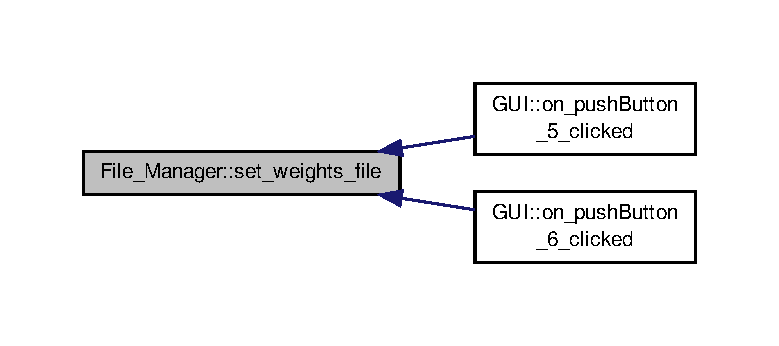
\includegraphics[width=350pt]{d8/d84/a00001_a860e5837e1671018a26fdc0ce43603b1_icgraph}
\end{center}
\end{figure}


\hypertarget{a00001_a4e104949ad8e8fd75c612313f857ee5a}{\index{File\-\_\-\-Manager@{File\-\_\-\-Manager}!write\-\_\-output@{write\-\_\-output}}
\index{write\-\_\-output@{write\-\_\-output}!File_Manager@{File\-\_\-\-Manager}}
\subsubsection[{write\-\_\-output}]{\setlength{\rightskip}{0pt plus 5cm}void File\-\_\-\-Manager\-::write\-\_\-output (
\begin{DoxyParamCaption}
\item[{string}]{file\-Path}
\end{DoxyParamCaption}
)\hspace{0.3cm}{\ttfamily [private]}}}\label{d8/d84/a00001_a4e104949ad8e8fd75c612313f857ee5a}


Write output\par
 Opens file file\-Path and write to it. 


\begin{DoxyParams}{Parameters}
{\em \mbox{[}file\-Path\mbox{]}} & File path to be wrote. \\
\hline
\end{DoxyParams}
\begin{DoxyPrecond}{Precondition}
Directory specified by file\-Path is accessible. 
\end{DoxyPrecond}
\begin{DoxyPostcond}{Postcondition}
Output file to be found in the specified directory. 
\end{DoxyPostcond}


Definition at line 126 of file F\-M.\-cpp.



References Neural\-\_\-\-Network\-::dataset\-\_\-size, fori, forj, n, Neural\-\_\-\-Network\-::output\-\_\-dataset, Neural\-\_\-\-Network\-::output\-\_\-len, output\-\_\-population\-\_\-string, Neural\-\_\-\-Network\-::rank\-\_\-output, and write.



Here is the caller graph for this function\-:\nopagebreak
\begin{figure}[H]
\begin{center}
\leavevmode
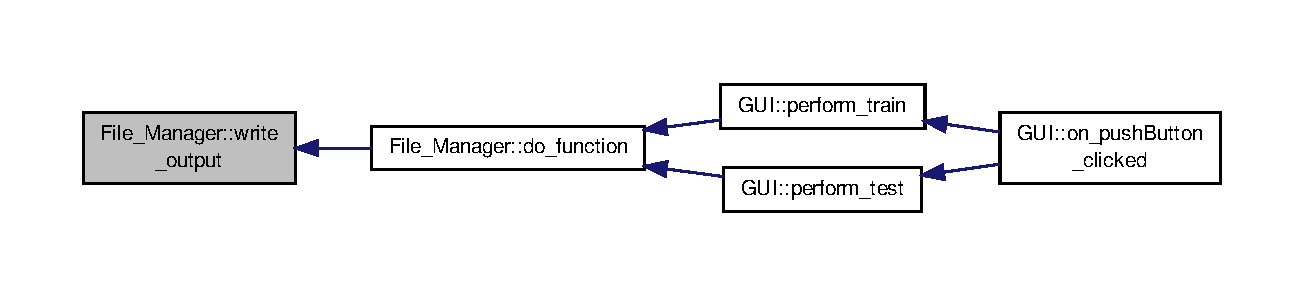
\includegraphics[width=350pt]{d8/d84/a00001_a4e104949ad8e8fd75c612313f857ee5a_icgraph}
\end{center}
\end{figure}


\hypertarget{a00001_a67e37c5e1429df91a8c4ff836579cdc0}{\index{File\-\_\-\-Manager@{File\-\_\-\-Manager}!write\-\_\-weights@{write\-\_\-weights}}
\index{write\-\_\-weights@{write\-\_\-weights}!File_Manager@{File\-\_\-\-Manager}}
\subsubsection[{write\-\_\-weights}]{\setlength{\rightskip}{0pt plus 5cm}void File\-\_\-\-Manager\-::write\-\_\-weights (
\begin{DoxyParamCaption}
\item[{string}]{file\-Path}
\end{DoxyParamCaption}
)\hspace{0.3cm}{\ttfamily [private]}}}\label{d8/d84/a00001_a67e37c5e1429df91a8c4ff836579cdc0}


Write weights\par
 Opens file file\-Path and write to it. 


\begin{DoxyParams}{Parameters}
{\em \mbox{[}file\-Path\mbox{]}} & File path to be wrote. \\
\hline
\end{DoxyParams}
\begin{DoxyPrecond}{Precondition}
Directory specified by file\-Path is accessible. 
\end{DoxyPrecond}
\begin{DoxyPostcond}{Postcondition}
Weights file to be found in the specified directory. 
\end{DoxyPostcond}


Definition at line 181 of file F\-M.\-cpp.



References fori, forj, Neural\-\_\-\-Network\-::hidden\-\_\-len, Neural\-\_\-\-Network\-::input\-\_\-len, n, Neural\-\_\-\-Network\-::output\-\_\-len, Neural\-\_\-\-Network\-::\-Wh, Neural\-\_\-\-Network\-::\-Wo, and write.



Here is the caller graph for this function\-:\nopagebreak
\begin{figure}[H]
\begin{center}
\leavevmode
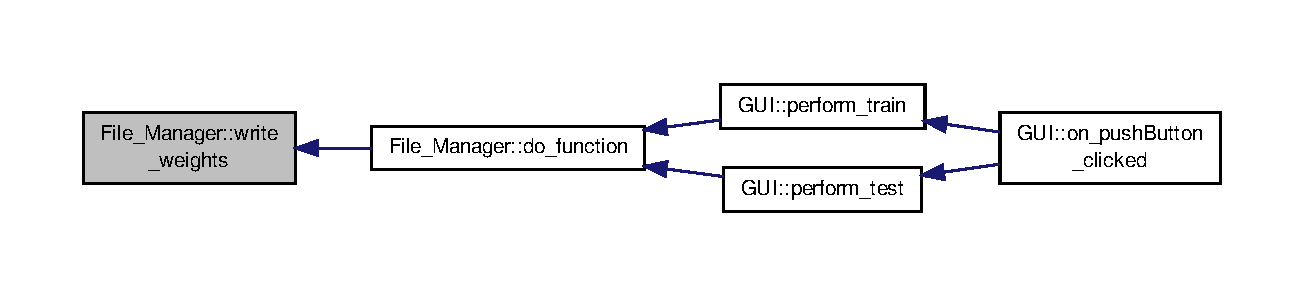
\includegraphics[width=350pt]{d8/d84/a00001_a67e37c5e1429df91a8c4ff836579cdc0_icgraph}
\end{center}
\end{figure}




\subsection{Member Data Documentation}
\hypertarget{a00001_a8b8f5c9cc3ffcb083ccc4fce1c05ca44}{\index{File\-\_\-\-Manager@{File\-\_\-\-Manager}!expected\-\_\-out\-\_\-file@{expected\-\_\-out\-\_\-file}}
\index{expected\-\_\-out\-\_\-file@{expected\-\_\-out\-\_\-file}!File_Manager@{File\-\_\-\-Manager}}
\subsubsection[{expected\-\_\-out\-\_\-file}]{\setlength{\rightskip}{0pt plus 5cm}string File\-\_\-\-Manager\-::expected\-\_\-out\-\_\-file\hspace{0.3cm}{\ttfamily [private]}}}\label{d8/d84/a00001_a8b8f5c9cc3ffcb083ccc4fce1c05ca44}


Definition at line 38 of file File\-Manager.\-h.

\hypertarget{a00001_a78b144182e3cfc70f9aae78ebdd66e51}{\index{File\-\_\-\-Manager@{File\-\_\-\-Manager}!input\-\_\-file@{input\-\_\-file}}
\index{input\-\_\-file@{input\-\_\-file}!File_Manager@{File\-\_\-\-Manager}}
\subsubsection[{input\-\_\-file}]{\setlength{\rightskip}{0pt plus 5cm}string File\-\_\-\-Manager\-::input\-\_\-file\hspace{0.3cm}{\ttfamily [private]}}}\label{d8/d84/a00001_a78b144182e3cfc70f9aae78ebdd66e51}


Definition at line 37 of file File\-Manager.\-h.

\hypertarget{a00001_a80f6d8f738cbc4d10154b470c5422fdd}{\index{File\-\_\-\-Manager@{File\-\_\-\-Manager}!input\-\_\-population\-\_\-string@{input\-\_\-population\-\_\-string}}
\index{input\-\_\-population\-\_\-string@{input\-\_\-population\-\_\-string}!File_Manager@{File\-\_\-\-Manager}}
\subsubsection[{input\-\_\-population\-\_\-string}]{\setlength{\rightskip}{0pt plus 5cm}string File\-\_\-\-Manager\-::input\-\_\-population\-\_\-string\hspace{0.3cm}{\ttfamily [private]}}}\label{d8/d84/a00001_a80f6d8f738cbc4d10154b470c5422fdd}


Definition at line 35 of file File\-Manager.\-h.

\hypertarget{a00001_ac70ea2427e95618bb3903b2c57ee9745}{\index{File\-\_\-\-Manager@{File\-\_\-\-Manager}!n@{n}}
\index{n@{n}!File_Manager@{File\-\_\-\-Manager}}
\subsubsection[{n}]{\setlength{\rightskip}{0pt plus 5cm}{\bf Neural\-\_\-\-Network} File\-\_\-\-Manager\-::n}}\label{d8/d84/a00001_ac70ea2427e95618bb3903b2c57ee9745}


Definition at line 12 of file File\-Manager.\-h.

\hypertarget{a00001_a63725670a06637b4290c54eba671b640}{\index{File\-\_\-\-Manager@{File\-\_\-\-Manager}!output\-\_\-file@{output\-\_\-file}}
\index{output\-\_\-file@{output\-\_\-file}!File_Manager@{File\-\_\-\-Manager}}
\subsubsection[{output\-\_\-file}]{\setlength{\rightskip}{0pt plus 5cm}string File\-\_\-\-Manager\-::output\-\_\-file\hspace{0.3cm}{\ttfamily [private]}}}\label{d8/d84/a00001_a63725670a06637b4290c54eba671b640}


Definition at line 39 of file File\-Manager.\-h.

\hypertarget{a00001_a4266a9bec2fff5d17d7abf06e00384db}{\index{File\-\_\-\-Manager@{File\-\_\-\-Manager}!output\-\_\-population\-\_\-string@{output\-\_\-population\-\_\-string}}
\index{output\-\_\-population\-\_\-string@{output\-\_\-population\-\_\-string}!File_Manager@{File\-\_\-\-Manager}}
\subsubsection[{output\-\_\-population\-\_\-string}]{\setlength{\rightskip}{0pt plus 5cm}string File\-\_\-\-Manager\-::output\-\_\-population\-\_\-string\hspace{0.3cm}{\ttfamily [private]}}}\label{d8/d84/a00001_a4266a9bec2fff5d17d7abf06e00384db}


Definition at line 36 of file File\-Manager.\-h.

\hypertarget{a00001_a578abb99a35121fea6c83f1dc21cc2af}{\index{File\-\_\-\-Manager@{File\-\_\-\-Manager}!rank\-\_\-output\-\_\-strings@{rank\-\_\-output\-\_\-strings}}
\index{rank\-\_\-output\-\_\-strings@{rank\-\_\-output\-\_\-strings}!File_Manager@{File\-\_\-\-Manager}}
\subsubsection[{rank\-\_\-output\-\_\-strings}]{\setlength{\rightskip}{0pt plus 5cm}string File\-\_\-\-Manager\-::rank\-\_\-output\-\_\-strings\mbox{[}{\bf output\-\_\-l}\mbox{]}\hspace{0.3cm}{\ttfamily [private]}}}\label{d8/d84/a00001_a578abb99a35121fea6c83f1dc21cc2af}


Definition at line 41 of file File\-Manager.\-h.

\hypertarget{a00001_a035fb2bdf99f8f928d049bc950c81f4c}{\index{File\-\_\-\-Manager@{File\-\_\-\-Manager}!read@{read}}
\index{read@{read}!File_Manager@{File\-\_\-\-Manager}}
\subsubsection[{read}]{\setlength{\rightskip}{0pt plus 5cm}ifstream File\-\_\-\-Manager\-::read\hspace{0.3cm}{\ttfamily [private]}}}\label{d8/d84/a00001_a035fb2bdf99f8f928d049bc950c81f4c}


Definition at line 33 of file File\-Manager.\-h.

\hypertarget{a00001_af7d8ea2c0a997e16600478c0020b1858}{\index{File\-\_\-\-Manager@{File\-\_\-\-Manager}!read\-\_\-ex\-\_\-output\-\_\-string@{read\-\_\-ex\-\_\-output\-\_\-string}}
\index{read\-\_\-ex\-\_\-output\-\_\-string@{read\-\_\-ex\-\_\-output\-\_\-string}!File_Manager@{File\-\_\-\-Manager}}
\subsubsection[{read\-\_\-ex\-\_\-output\-\_\-string}]{\setlength{\rightskip}{0pt plus 5cm}string File\-\_\-\-Manager\-::read\-\_\-ex\-\_\-output\-\_\-string\hspace{0.3cm}{\ttfamily [private]}}}\label{d8/d84/a00001_af7d8ea2c0a997e16600478c0020b1858}


Definition at line 34 of file File\-Manager.\-h.

\hypertarget{a00001_aab02256124e6eb39e10e3c9765f0bcb3}{\index{File\-\_\-\-Manager@{File\-\_\-\-Manager}!weights\-\_\-file@{weights\-\_\-file}}
\index{weights\-\_\-file@{weights\-\_\-file}!File_Manager@{File\-\_\-\-Manager}}
\subsubsection[{weights\-\_\-file}]{\setlength{\rightskip}{0pt plus 5cm}string File\-\_\-\-Manager\-::weights\-\_\-file\hspace{0.3cm}{\ttfamily [private]}}}\label{d8/d84/a00001_aab02256124e6eb39e10e3c9765f0bcb3}


Definition at line 40 of file File\-Manager.\-h.

\hypertarget{a00001_a7d29cb8d04a1a60638f653c28a628095}{\index{File\-\_\-\-Manager@{File\-\_\-\-Manager}!write@{write}}
\index{write@{write}!File_Manager@{File\-\_\-\-Manager}}
\subsubsection[{write}]{\setlength{\rightskip}{0pt plus 5cm}ofstream File\-\_\-\-Manager\-::write\hspace{0.3cm}{\ttfamily [private]}}}\label{d8/d84/a00001_a7d29cb8d04a1a60638f653c28a628095}


Definition at line 32 of file File\-Manager.\-h.



The documentation for this class was generated from the following files\-:\begin{DoxyCompactItemize}
\item 
phenogene/\hyperlink{a00004}{File\-Manager.\-h}\item 
phenogene/\hyperlink{a00005}{F\-M.\-cpp}\item 
phenogene/\hyperlink{a00006}{F\-M\-\_\-getters.\-cpp}\item 
phenogene/\hyperlink{a00007}{F\-M\-\_\-setters.\-cpp}\end{DoxyCompactItemize}

\hypertarget{a00002}{\section{G\-U\-I Class Reference}
\label{d7/d46/a00002}\index{G\-U\-I@{G\-U\-I}}
}


{\ttfamily \#include $<$G\-U\-I.\-h$>$}



Collaboration diagram for G\-U\-I\-:\nopagebreak
\begin{figure}[H]
\begin{center}
\leavevmode
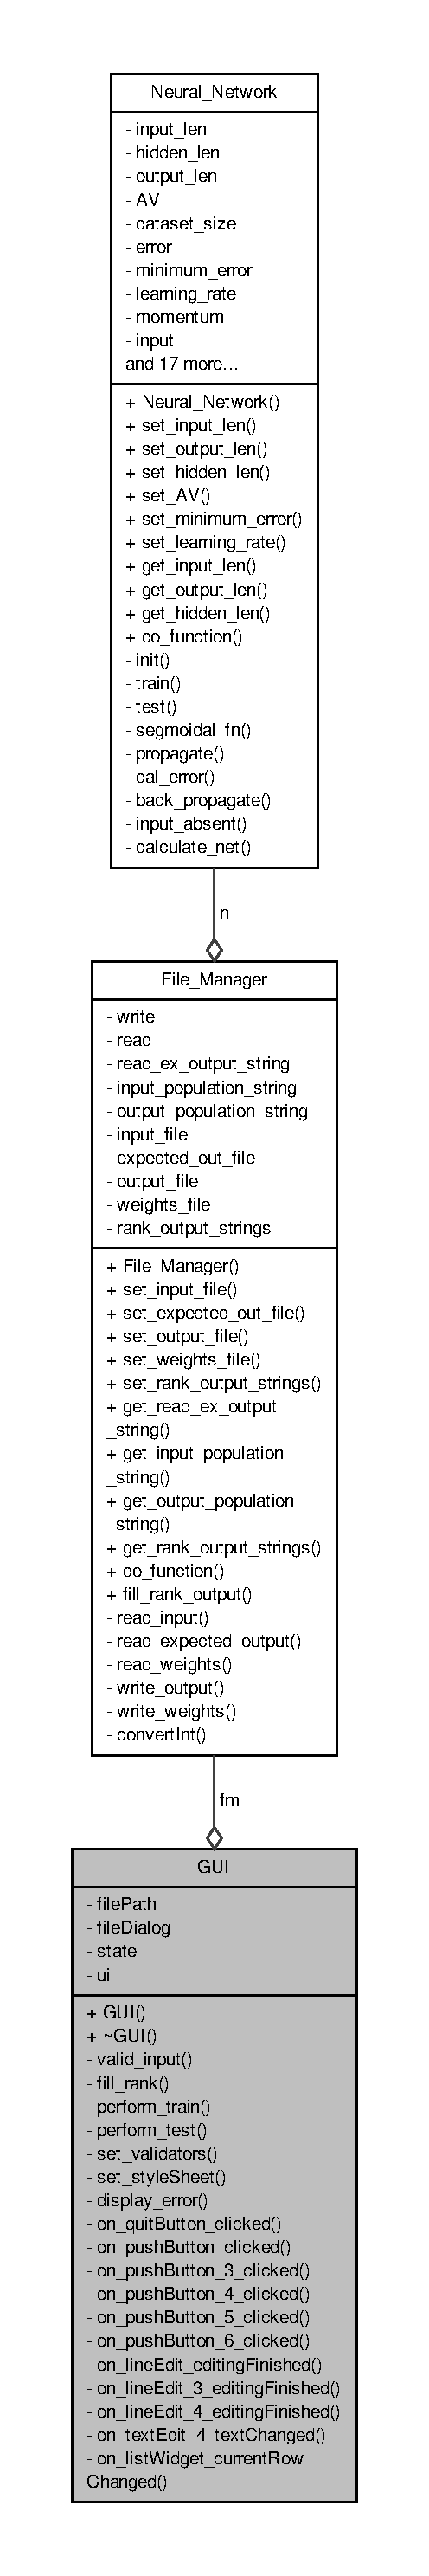
\includegraphics[height=550pt]{d5/df9/a00044}
\end{center}
\end{figure}
\subsection*{Public Member Functions}
\begin{DoxyCompactItemize}
\item 
\hyperlink{a00002_acb0ba8c6fc121d814d30560e2c29f2fe}{G\-U\-I} (Q\-Widget $\ast$parent=0)
\begin{DoxyCompactList}\small\item\em \hyperlink{a00002}{G\-U\-I} class constructor. \end{DoxyCompactList}\item 
\hyperlink{a00002_ac9cae2328dcb5d83bdfaeca49a2eb695}{$\sim$\-G\-U\-I} ()
\end{DoxyCompactItemize}
\subsection*{Private Slots}
\begin{DoxyCompactItemize}
\item 
void \hyperlink{a00002_a5acc81766a1842665846092ebf0815e0}{on\-\_\-quit\-Button\-\_\-clicked} ()
\item 
void \hyperlink{a00002_a043466f485b6b75ee25ee879121c1ecc}{on\-\_\-push\-Button\-\_\-clicked} ()
\begin{DoxyCompactList}\small\item\em Called when start button is pushed.\par
 Determines weather to train/test/analyze, according to the opened tab. \end{DoxyCompactList}\item 
void \hyperlink{a00002_a09eeb721e4f861e80da92d8ed42277ee}{on\-\_\-push\-Button\-\_\-3\-\_\-clicked} ()
\begin{DoxyCompactList}\small\item\em Browses Expected Output File\par
 Allows the user to select a file. \end{DoxyCompactList}\item 
void \hyperlink{a00002_a9a338258e3edb0d5ab1aabc26dd34d40}{on\-\_\-push\-Button\-\_\-4\-\_\-clicked} ()
\begin{DoxyCompactList}\small\item\em Browses Input File\par
 Allows the user to select a file. \end{DoxyCompactList}\item 
void \hyperlink{a00002_a6fd99e6dc89a1f3d352c037c880ef345}{on\-\_\-push\-Button\-\_\-5\-\_\-clicked} ()
\begin{DoxyCompactList}\small\item\em Browses Input File\par
 Allows the user to select a file. \end{DoxyCompactList}\item 
void \hyperlink{a00002_a8b08d8812751902c52d56efc45d0b58d}{on\-\_\-push\-Button\-\_\-6\-\_\-clicked} ()
\begin{DoxyCompactList}\small\item\em Browses Weights File\par
 Allows the user to select a file. \end{DoxyCompactList}\item 
void \hyperlink{a00002_ab5da77a34a83e9794edda0d77d79bec0}{on\-\_\-line\-Edit\-\_\-editing\-Finished} ()
\begin{DoxyCompactList}\small\item\em Set gene number, aka, input nodes number. \end{DoxyCompactList}\item 
void \hyperlink{a00002_a6aff5c3694d19ebd2bd81010c239cf62}{on\-\_\-line\-Edit\-\_\-3\-\_\-editing\-Finished} ()
\begin{DoxyCompactList}\small\item\em Set learning rate. \end{DoxyCompactList}\item 
void \hyperlink{a00002_a6bcefb22fdfb8fbd3146eab38a0023d7}{on\-\_\-line\-Edit\-\_\-4\-\_\-editing\-Finished} ()
\begin{DoxyCompactList}\small\item\em Set Acceptable Error. \end{DoxyCompactList}\item 
void \hyperlink{a00002_a39f58394bb8e9691a7b32774114a910a}{on\-\_\-text\-Edit\-\_\-4\-\_\-text\-Changed} ()
\begin{DoxyCompactList}\small\item\em Set output keywords. \end{DoxyCompactList}\item 
void \hyperlink{a00002_a073c74e8357311d12c523d73414ee265}{on\-\_\-list\-Widget\-\_\-current\-Row\-Changed} (int current\-Row)
\end{DoxyCompactItemize}
\subsection*{Private Member Functions}
\begin{DoxyCompactItemize}
\item 
Q\-String \hyperlink{a00002_a5ec9d8a051303b218c4542f96a87b56f}{valid\-\_\-input} ()
\begin{DoxyCompactList}\small\item\em Check that all input needed is filled. \end{DoxyCompactList}\item 
void \hyperlink{a00002_a8e8c5918a3a0ddfd352c62e7348d3d74}{fill\-\_\-rank} ()
\begin{DoxyCompactList}\small\item\em Called once before a train/test is performed. \end{DoxyCompactList}\item 
void \hyperlink{a00002_ad1bb069dee02010a61045c91f5e7752f}{perform\-\_\-train} ()
\begin{DoxyCompactList}\small\item\em Calls file manager rotines to train\-:\par
. \end{DoxyCompactList}\item 
void \hyperlink{a00002_ade6ba53055965b3522fa3cd022e4c5e0}{perform\-\_\-test} ()
\item 
void \hyperlink{a00002_abd9fac4d8ad5334cc48afb0513544898}{set\-\_\-validators} ()
\begin{DoxyCompactList}\small\item\em Set validators for user input. \end{DoxyCompactList}\item 
void \hyperlink{a00002_a5683a1862ec1a85cf87d9c5f6fc528e9}{set\-\_\-style\-Sheet} ()
\begin{DoxyCompactList}\small\item\em Set style sheet configuration\-: Set color grey for some labels. \end{DoxyCompactList}\item 
void \hyperlink{a00002_a69ac504cf1500a8c6283d8721b09aeb2}{display\-\_\-error} (Q\-String)
\begin{DoxyCompactList}\small\item\em Displays the error message contained in string er. \end{DoxyCompactList}\end{DoxyCompactItemize}
\subsection*{Private Attributes}
\begin{DoxyCompactItemize}
\item 
Q\-String \hyperlink{a00002_a62d0a4c604ed8d65f85455971a938548}{file\-Path}
\item 
Q\-File\-Dialog \hyperlink{a00002_a9ed0a8b583419e88bb94697a9b258c72}{file\-Dialog}
\item 
Q\-Byte\-Array \hyperlink{a00002_aa3abed87f53b22188d76a134e427b30d}{state}
\item 
Ui\-::\-G\-U\-I $\ast$ \hyperlink{a00002_acdbca1224663f5a19bd1ad4e7c885886}{ui}
\item 
\hyperlink{a00001}{File\-\_\-\-Manager} \hyperlink{a00002_a73cc90505024488d2fd77762ad5059c4}{fm}
\end{DoxyCompactItemize}


\subsection{Detailed Description}


Definition at line 18 of file G\-U\-I.\-h.



\subsection{Constructor \& Destructor Documentation}
\hypertarget{a00002_acb0ba8c6fc121d814d30560e2c29f2fe}{\index{G\-U\-I@{G\-U\-I}!G\-U\-I@{G\-U\-I}}
\index{G\-U\-I@{G\-U\-I}!GUI@{G\-U\-I}}
\subsubsection[{G\-U\-I}]{\setlength{\rightskip}{0pt plus 5cm}G\-U\-I\-::\-G\-U\-I (
\begin{DoxyParamCaption}
\item[{Q\-Widget $\ast$}]{parent = {\ttfamily 0}}
\end{DoxyParamCaption}
)\hspace{0.3cm}{\ttfamily [explicit]}}}\label{d7/d46/a00002_acb0ba8c6fc121d814d30560e2c29f2fe}


\hyperlink{a00002}{G\-U\-I} class constructor. 



Definition at line 8 of file G\-U\-I\-\_\-constructor.\-cpp.



References set\-\_\-style\-Sheet(), and set\-\_\-validators().



Here is the call graph for this function\-:\nopagebreak
\begin{figure}[H]
\begin{center}
\leavevmode
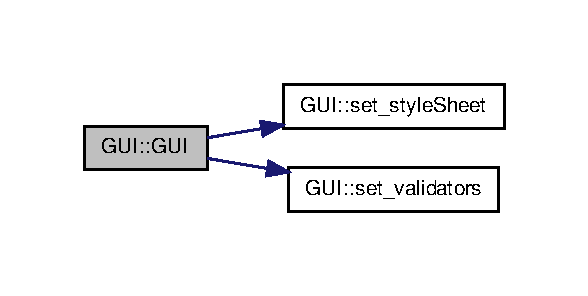
\includegraphics[width=282pt]{d7/d46/a00002_acb0ba8c6fc121d814d30560e2c29f2fe_cgraph}
\end{center}
\end{figure}


\hypertarget{a00002_ac9cae2328dcb5d83bdfaeca49a2eb695}{\index{G\-U\-I@{G\-U\-I}!$\sim$\-G\-U\-I@{$\sim$\-G\-U\-I}}
\index{$\sim$\-G\-U\-I@{$\sim$\-G\-U\-I}!GUI@{G\-U\-I}}
\subsubsection[{$\sim$\-G\-U\-I}]{\setlength{\rightskip}{0pt plus 5cm}G\-U\-I\-::$\sim$\-G\-U\-I (
\begin{DoxyParamCaption}
{}
\end{DoxyParamCaption}
)}}\label{d7/d46/a00002_ac9cae2328dcb5d83bdfaeca49a2eb695}


Definition at line 47 of file G\-U\-I\-\_\-constructor.\-cpp.



References ui.



\subsection{Member Function Documentation}
\hypertarget{a00002_a69ac504cf1500a8c6283d8721b09aeb2}{\index{G\-U\-I@{G\-U\-I}!display\-\_\-error@{display\-\_\-error}}
\index{display\-\_\-error@{display\-\_\-error}!GUI@{G\-U\-I}}
\subsubsection[{display\-\_\-error}]{\setlength{\rightskip}{0pt plus 5cm}void G\-U\-I\-::display\-\_\-error (
\begin{DoxyParamCaption}
\item[{Q\-String}]{er}
\end{DoxyParamCaption}
)\hspace{0.3cm}{\ttfamily [private]}}}\label{d7/d46/a00002_a69ac504cf1500a8c6283d8721b09aeb2}


Displays the error message contained in string er. 


\begin{DoxyParams}{Parameters}
{\em \mbox{[}\-Qstring} & er\mbox{]} Error message to be displayed. \\
\hline
\end{DoxyParams}


Definition at line 131 of file G\-U\-I\-\_\-start\-Button.\-cpp.



Here is the caller graph for this function\-:\nopagebreak
\begin{figure}[H]
\begin{center}
\leavevmode
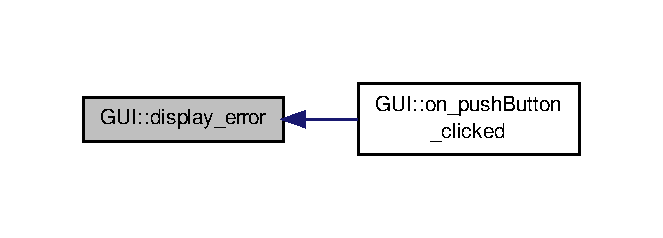
\includegraphics[width=318pt]{d7/d46/a00002_a69ac504cf1500a8c6283d8721b09aeb2_icgraph}
\end{center}
\end{figure}


\hypertarget{a00002_a8e8c5918a3a0ddfd352c62e7348d3d74}{\index{G\-U\-I@{G\-U\-I}!fill\-\_\-rank@{fill\-\_\-rank}}
\index{fill\-\_\-rank@{fill\-\_\-rank}!GUI@{G\-U\-I}}
\subsubsection[{fill\-\_\-rank}]{\setlength{\rightskip}{0pt plus 5cm}void G\-U\-I\-::fill\-\_\-rank (
\begin{DoxyParamCaption}
{}
\end{DoxyParamCaption}
)\hspace{0.3cm}{\ttfamily [private]}}}\label{d7/d46/a00002_a8e8c5918a3a0ddfd352c62e7348d3d74}


Called once before a train/test is performed. 

\begin{DoxyPostcond}{Postcondition}
Rank-\/\-Output Strings are filled. 
\end{DoxyPostcond}


Definition at line 116 of file G\-U\-I\-\_\-start\-Button.\-cpp.



References fm, File\-\_\-\-Manager\-::set\-\_\-rank\-\_\-output\-\_\-strings(), and ui.



Here is the call graph for this function\-:\nopagebreak
\begin{figure}[H]
\begin{center}
\leavevmode
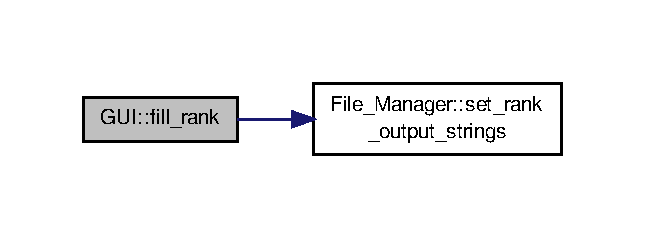
\includegraphics[width=310pt]{d7/d46/a00002_a8e8c5918a3a0ddfd352c62e7348d3d74_cgraph}
\end{center}
\end{figure}




Here is the caller graph for this function\-:
\nopagebreak
\begin{figure}[H]
\begin{center}
\leavevmode
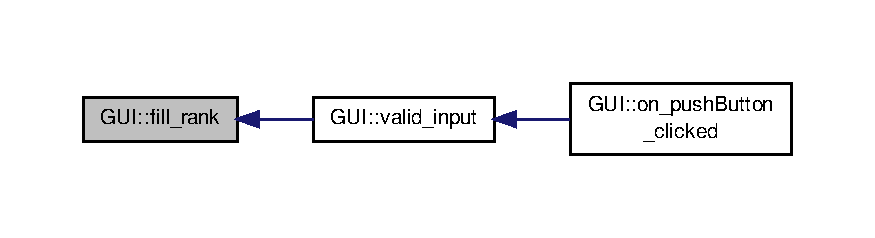
\includegraphics[width=350pt]{d7/d46/a00002_a8e8c5918a3a0ddfd352c62e7348d3d74_icgraph}
\end{center}
\end{figure}


\hypertarget{a00002_a6aff5c3694d19ebd2bd81010c239cf62}{\index{G\-U\-I@{G\-U\-I}!on\-\_\-line\-Edit\-\_\-3\-\_\-editing\-Finished@{on\-\_\-line\-Edit\-\_\-3\-\_\-editing\-Finished}}
\index{on\-\_\-line\-Edit\-\_\-3\-\_\-editing\-Finished@{on\-\_\-line\-Edit\-\_\-3\-\_\-editing\-Finished}!GUI@{G\-U\-I}}
\subsubsection[{on\-\_\-line\-Edit\-\_\-3\-\_\-editing\-Finished}]{\setlength{\rightskip}{0pt plus 5cm}void G\-U\-I\-::on\-\_\-line\-Edit\-\_\-3\-\_\-editing\-Finished (
\begin{DoxyParamCaption}
{}
\end{DoxyParamCaption}
)\hspace{0.3cm}{\ttfamily [private]}, {\ttfamily [slot]}}}\label{d7/d46/a00002_a6aff5c3694d19ebd2bd81010c239cf62}


Set learning rate. 

On Train Tab \begin{DoxyPrecond}{Precondition}
Entered is a valid double number. 
\end{DoxyPrecond}
\begin{DoxyPostcond}{Postcondition}
Learning rate is set. 
\end{DoxyPostcond}


Definition at line 61 of file G\-U\-I.\-cpp.



References fm, File\-\_\-\-Manager\-::n, Neural\-\_\-\-Network\-::set\-\_\-learning\-\_\-rate(), and ui.



Here is the call graph for this function\-:\nopagebreak
\begin{figure}[H]
\begin{center}
\leavevmode
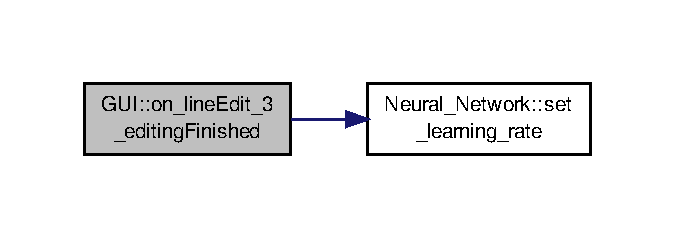
\includegraphics[width=324pt]{d7/d46/a00002_a6aff5c3694d19ebd2bd81010c239cf62_cgraph}
\end{center}
\end{figure}


\hypertarget{a00002_a6bcefb22fdfb8fbd3146eab38a0023d7}{\index{G\-U\-I@{G\-U\-I}!on\-\_\-line\-Edit\-\_\-4\-\_\-editing\-Finished@{on\-\_\-line\-Edit\-\_\-4\-\_\-editing\-Finished}}
\index{on\-\_\-line\-Edit\-\_\-4\-\_\-editing\-Finished@{on\-\_\-line\-Edit\-\_\-4\-\_\-editing\-Finished}!GUI@{G\-U\-I}}
\subsubsection[{on\-\_\-line\-Edit\-\_\-4\-\_\-editing\-Finished}]{\setlength{\rightskip}{0pt plus 5cm}void G\-U\-I\-::on\-\_\-line\-Edit\-\_\-4\-\_\-editing\-Finished (
\begin{DoxyParamCaption}
{}
\end{DoxyParamCaption}
)\hspace{0.3cm}{\ttfamily [private]}, {\ttfamily [slot]}}}\label{d7/d46/a00002_a6bcefb22fdfb8fbd3146eab38a0023d7}


Set Acceptable Error. 

On Train Tab \begin{DoxyPrecond}{Precondition}
Entered is a valid double number. 
\end{DoxyPrecond}
\begin{DoxyPostcond}{Postcondition}
Minimum error is set. 
\end{DoxyPostcond}


Definition at line 73 of file G\-U\-I.\-cpp.



References fm, File\-\_\-\-Manager\-::n, Neural\-\_\-\-Network\-::set\-\_\-minimum\-\_\-error(), and ui.



Here is the call graph for this function\-:\nopagebreak
\begin{figure}[H]
\begin{center}
\leavevmode
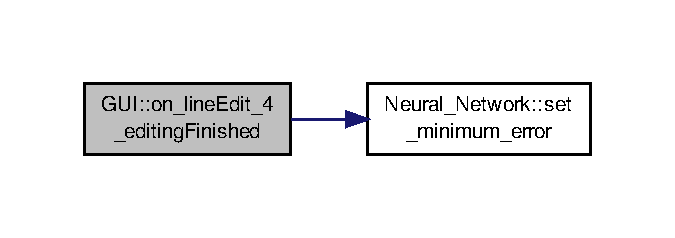
\includegraphics[width=324pt]{d7/d46/a00002_a6bcefb22fdfb8fbd3146eab38a0023d7_cgraph}
\end{center}
\end{figure}


\hypertarget{a00002_ab5da77a34a83e9794edda0d77d79bec0}{\index{G\-U\-I@{G\-U\-I}!on\-\_\-line\-Edit\-\_\-editing\-Finished@{on\-\_\-line\-Edit\-\_\-editing\-Finished}}
\index{on\-\_\-line\-Edit\-\_\-editing\-Finished@{on\-\_\-line\-Edit\-\_\-editing\-Finished}!GUI@{G\-U\-I}}
\subsubsection[{on\-\_\-line\-Edit\-\_\-editing\-Finished}]{\setlength{\rightskip}{0pt plus 5cm}void G\-U\-I\-::on\-\_\-line\-Edit\-\_\-editing\-Finished (
\begin{DoxyParamCaption}
{}
\end{DoxyParamCaption}
)\hspace{0.3cm}{\ttfamily [private]}, {\ttfamily [slot]}}}\label{d7/d46/a00002_ab5da77a34a83e9794edda0d77d79bec0}


Set gene number, aka, input nodes number. 

On Train Tab \begin{DoxyPrecond}{Precondition}
Entered is a valid integer number. 
\end{DoxyPrecond}
\begin{DoxyPostcond}{Postcondition}
Input nodes number is set. 
\end{DoxyPostcond}


Definition at line 48 of file G\-U\-I.\-cpp.



References fm, File\-\_\-\-Manager\-::n, Neural\-\_\-\-Network\-::set\-\_\-input\-\_\-len(), and ui.



Here is the call graph for this function\-:\nopagebreak
\begin{figure}[H]
\begin{center}
\leavevmode
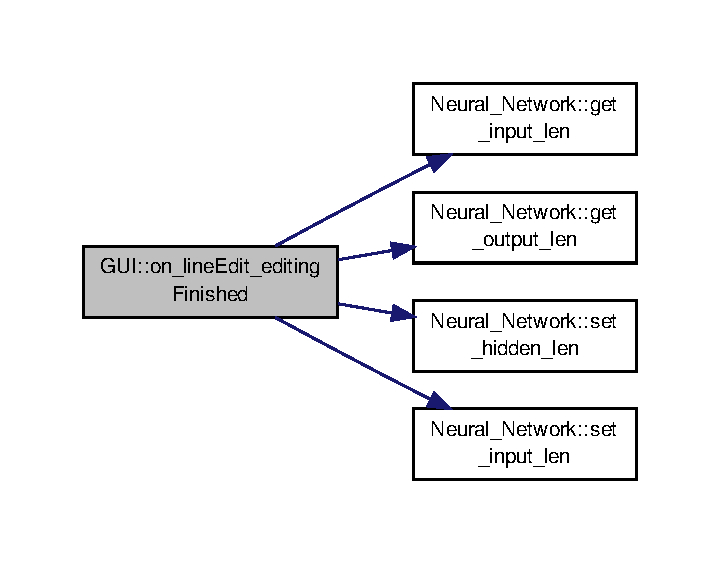
\includegraphics[width=346pt]{d7/d46/a00002_ab5da77a34a83e9794edda0d77d79bec0_cgraph}
\end{center}
\end{figure}


\hypertarget{a00002_a073c74e8357311d12c523d73414ee265}{\index{G\-U\-I@{G\-U\-I}!on\-\_\-list\-Widget\-\_\-current\-Row\-Changed@{on\-\_\-list\-Widget\-\_\-current\-Row\-Changed}}
\index{on\-\_\-list\-Widget\-\_\-current\-Row\-Changed@{on\-\_\-list\-Widget\-\_\-current\-Row\-Changed}!GUI@{G\-U\-I}}
\subsubsection[{on\-\_\-list\-Widget\-\_\-current\-Row\-Changed}]{\setlength{\rightskip}{0pt plus 5cm}void G\-U\-I\-::on\-\_\-list\-Widget\-\_\-current\-Row\-Changed (
\begin{DoxyParamCaption}
\item[{int}]{current\-Row}
\end{DoxyParamCaption}
)\hspace{0.3cm}{\ttfamily [private]}, {\ttfamily [slot]}}}\label{d7/d46/a00002_a073c74e8357311d12c523d73414ee265}


Definition at line 85 of file G\-U\-I.\-cpp.



References fm, File\-\_\-\-Manager\-::n, Neural\-\_\-\-Network\-::set\-\_\-\-A\-V(), and ui.



Here is the call graph for this function\-:\nopagebreak
\begin{figure}[H]
\begin{center}
\leavevmode
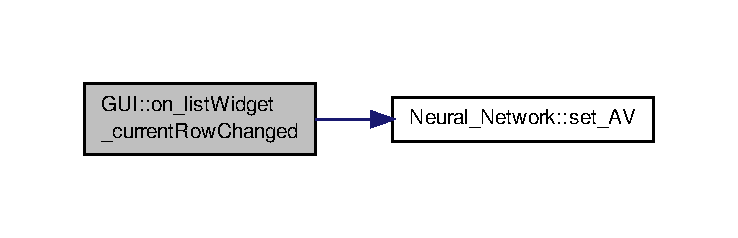
\includegraphics[width=350pt]{d7/d46/a00002_a073c74e8357311d12c523d73414ee265_cgraph}
\end{center}
\end{figure}


\hypertarget{a00002_a09eeb721e4f861e80da92d8ed42277ee}{\index{G\-U\-I@{G\-U\-I}!on\-\_\-push\-Button\-\_\-3\-\_\-clicked@{on\-\_\-push\-Button\-\_\-3\-\_\-clicked}}
\index{on\-\_\-push\-Button\-\_\-3\-\_\-clicked@{on\-\_\-push\-Button\-\_\-3\-\_\-clicked}!GUI@{G\-U\-I}}
\subsubsection[{on\-\_\-push\-Button\-\_\-3\-\_\-clicked}]{\setlength{\rightskip}{0pt plus 5cm}void G\-U\-I\-::on\-\_\-push\-Button\-\_\-3\-\_\-clicked (
\begin{DoxyParamCaption}
{}
\end{DoxyParamCaption}
)\hspace{0.3cm}{\ttfamily [private]}, {\ttfamily [slot]}}}\label{d7/d46/a00002_a09eeb721e4f861e80da92d8ed42277ee}


Browses Expected Output File\par
 Allows the user to select a file. 

On Train Tab \begin{DoxyPrecond}{Precondition}
Expected-\/\-Output browse button is clicked. 
\end{DoxyPrecond}
\begin{DoxyPostcond}{Postcondition}
File path to expected output file is set. 
\end{DoxyPostcond}


Definition at line 33 of file G\-U\-I.\-cpp.



References file\-Dialog, file\-Path, fm, File\-\_\-\-Manager\-::set\-\_\-expected\-\_\-out\-\_\-file(), and ui.



Here is the call graph for this function\-:\nopagebreak
\begin{figure}[H]
\begin{center}
\leavevmode
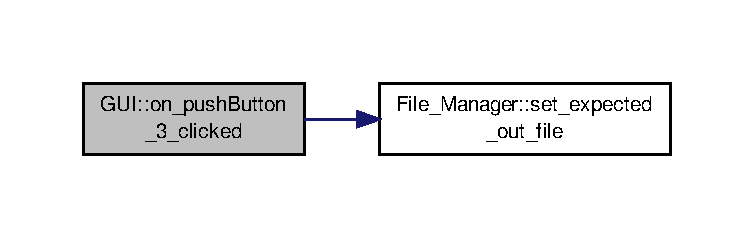
\includegraphics[width=350pt]{d7/d46/a00002_a09eeb721e4f861e80da92d8ed42277ee_cgraph}
\end{center}
\end{figure}


\hypertarget{a00002_a9a338258e3edb0d5ab1aabc26dd34d40}{\index{G\-U\-I@{G\-U\-I}!on\-\_\-push\-Button\-\_\-4\-\_\-clicked@{on\-\_\-push\-Button\-\_\-4\-\_\-clicked}}
\index{on\-\_\-push\-Button\-\_\-4\-\_\-clicked@{on\-\_\-push\-Button\-\_\-4\-\_\-clicked}!GUI@{G\-U\-I}}
\subsubsection[{on\-\_\-push\-Button\-\_\-4\-\_\-clicked}]{\setlength{\rightskip}{0pt plus 5cm}void G\-U\-I\-::on\-\_\-push\-Button\-\_\-4\-\_\-clicked (
\begin{DoxyParamCaption}
{}
\end{DoxyParamCaption}
)\hspace{0.3cm}{\ttfamily [private]}, {\ttfamily [slot]}}}\label{d7/d46/a00002_a9a338258e3edb0d5ab1aabc26dd34d40}


Browses Input File\par
 Allows the user to select a file. 

On Predict Tab \begin{DoxyPrecond}{Precondition}
Input browse button is clicked. 
\end{DoxyPrecond}
\begin{DoxyPostcond}{Postcondition}
File path to input file is set. 
\end{DoxyPostcond}


Definition at line 120 of file G\-U\-I.\-cpp.



References file\-Dialog, file\-Path, fm, File\-\_\-\-Manager\-::set\-\_\-input\-\_\-file(), File\-\_\-\-Manager\-::set\-\_\-output\-\_\-file(), and ui.



Here is the call graph for this function\-:\nopagebreak
\begin{figure}[H]
\begin{center}
\leavevmode
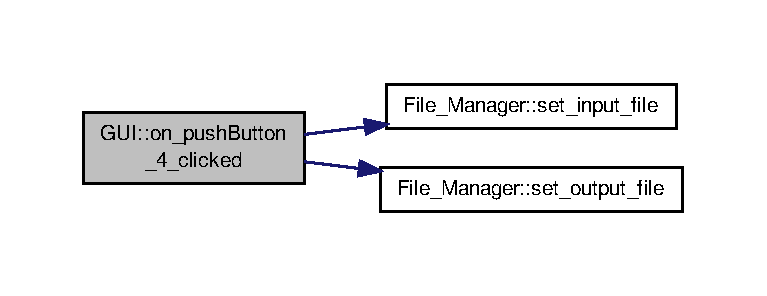
\includegraphics[width=350pt]{d7/d46/a00002_a9a338258e3edb0d5ab1aabc26dd34d40_cgraph}
\end{center}
\end{figure}


\hypertarget{a00002_a6fd99e6dc89a1f3d352c037c880ef345}{\index{G\-U\-I@{G\-U\-I}!on\-\_\-push\-Button\-\_\-5\-\_\-clicked@{on\-\_\-push\-Button\-\_\-5\-\_\-clicked}}
\index{on\-\_\-push\-Button\-\_\-5\-\_\-clicked@{on\-\_\-push\-Button\-\_\-5\-\_\-clicked}!GUI@{G\-U\-I}}
\subsubsection[{on\-\_\-push\-Button\-\_\-5\-\_\-clicked}]{\setlength{\rightskip}{0pt plus 5cm}void G\-U\-I\-::on\-\_\-push\-Button\-\_\-5\-\_\-clicked (
\begin{DoxyParamCaption}
{}
\end{DoxyParamCaption}
)\hspace{0.3cm}{\ttfamily [private]}, {\ttfamily [slot]}}}\label{d7/d46/a00002_a6fd99e6dc89a1f3d352c037c880ef345}


Browses Input File\par
 Allows the user to select a file. 

On Train Tab \begin{DoxyPrecond}{Precondition}
Input browse button is clicked. 
\end{DoxyPrecond}
\begin{DoxyPostcond}{Postcondition}
File path to input file is set. 
\end{DoxyPostcond}


Definition at line 12 of file G\-U\-I.\-cpp.



References file\-Dialog, file\-Path, fm, File\-\_\-\-Manager\-::set\-\_\-input\-\_\-file(), File\-\_\-\-Manager\-::set\-\_\-output\-\_\-file(), File\-\_\-\-Manager\-::set\-\_\-weights\-\_\-file(), and ui.



Here is the call graph for this function\-:\nopagebreak
\begin{figure}[H]
\begin{center}
\leavevmode
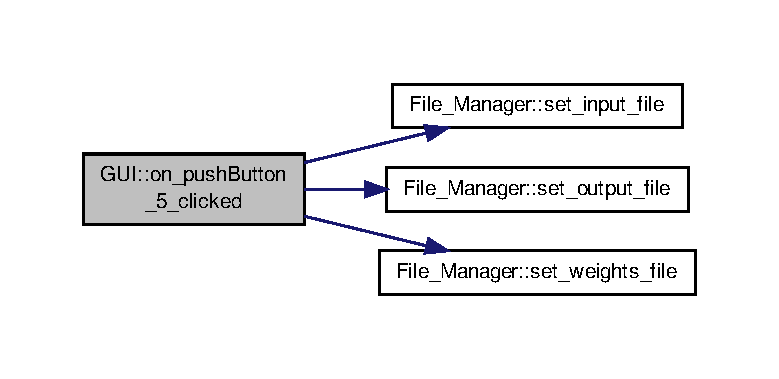
\includegraphics[width=350pt]{d7/d46/a00002_a6fd99e6dc89a1f3d352c037c880ef345_cgraph}
\end{center}
\end{figure}


\hypertarget{a00002_a8b08d8812751902c52d56efc45d0b58d}{\index{G\-U\-I@{G\-U\-I}!on\-\_\-push\-Button\-\_\-6\-\_\-clicked@{on\-\_\-push\-Button\-\_\-6\-\_\-clicked}}
\index{on\-\_\-push\-Button\-\_\-6\-\_\-clicked@{on\-\_\-push\-Button\-\_\-6\-\_\-clicked}!GUI@{G\-U\-I}}
\subsubsection[{on\-\_\-push\-Button\-\_\-6\-\_\-clicked}]{\setlength{\rightskip}{0pt plus 5cm}void G\-U\-I\-::on\-\_\-push\-Button\-\_\-6\-\_\-clicked (
\begin{DoxyParamCaption}
{}
\end{DoxyParamCaption}
)\hspace{0.3cm}{\ttfamily [private]}, {\ttfamily [slot]}}}\label{d7/d46/a00002_a8b08d8812751902c52d56efc45d0b58d}


Browses Weights File\par
 Allows the user to select a file. 

On Predict Tab \begin{DoxyPrecond}{Precondition}
Weights change button is clicked. 
\end{DoxyPrecond}
\begin{DoxyPostcond}{Postcondition}
File path to weights file is set. 
\end{DoxyPostcond}


Definition at line 137 of file G\-U\-I.\-cpp.



References file\-Dialog, file\-Path, fm, File\-\_\-\-Manager\-::set\-\_\-weights\-\_\-file(), and ui.



Here is the call graph for this function\-:\nopagebreak
\begin{figure}[H]
\begin{center}
\leavevmode
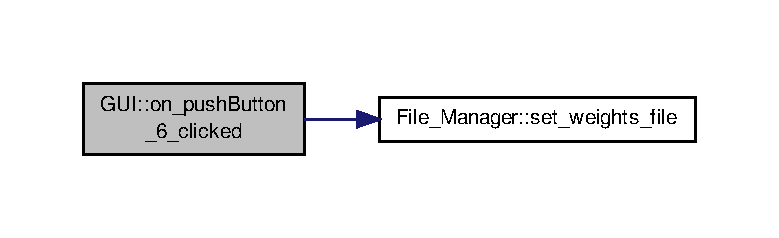
\includegraphics[width=350pt]{d7/d46/a00002_a8b08d8812751902c52d56efc45d0b58d_cgraph}
\end{center}
\end{figure}


\hypertarget{a00002_a043466f485b6b75ee25ee879121c1ecc}{\index{G\-U\-I@{G\-U\-I}!on\-\_\-push\-Button\-\_\-clicked@{on\-\_\-push\-Button\-\_\-clicked}}
\index{on\-\_\-push\-Button\-\_\-clicked@{on\-\_\-push\-Button\-\_\-clicked}!GUI@{G\-U\-I}}
\subsubsection[{on\-\_\-push\-Button\-\_\-clicked}]{\setlength{\rightskip}{0pt plus 5cm}void G\-U\-I\-::on\-\_\-push\-Button\-\_\-clicked (
\begin{DoxyParamCaption}
{}
\end{DoxyParamCaption}
)\hspace{0.3cm}{\ttfamily [private]}, {\ttfamily [slot]}}}\label{d7/d46/a00002_a043466f485b6b75ee25ee879121c1ecc}


Called when start button is pushed.\par
 Determines weather to train/test/analyze, according to the opened tab. 



Definition at line 9 of file G\-U\-I\-\_\-start\-Button.\-cpp.



References display\-\_\-error(), File\-\_\-\-Manager\-::fill\-\_\-rank\-\_\-output(), fm, perform\-\_\-test(), perform\-\_\-train(), ui, and valid\-\_\-input().



Here is the call graph for this function\-:
\nopagebreak
\begin{figure}[H]
\begin{center}
\leavevmode
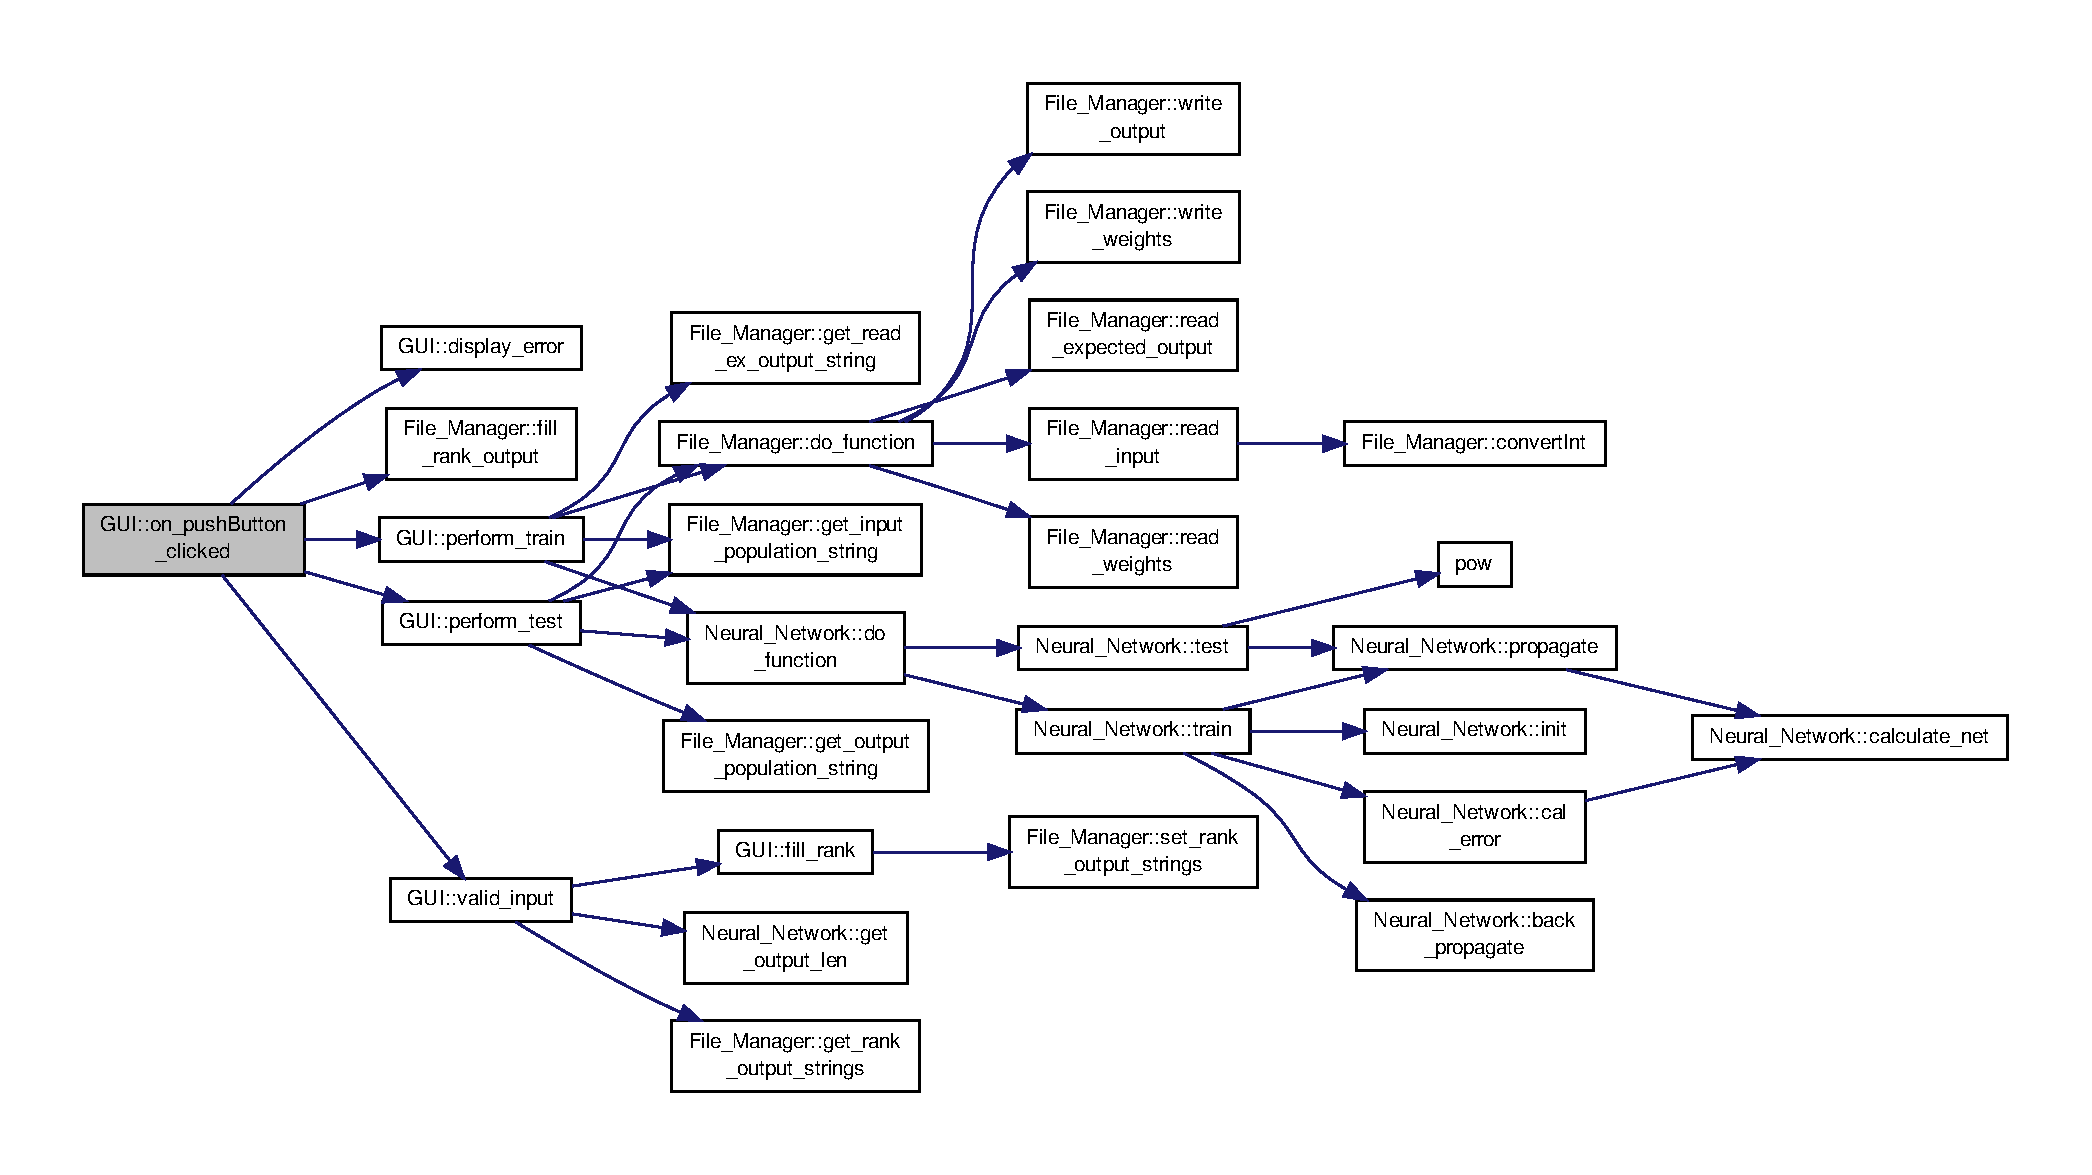
\includegraphics[width=350pt]{d7/d46/a00002_a043466f485b6b75ee25ee879121c1ecc_cgraph}
\end{center}
\end{figure}


\hypertarget{a00002_a5acc81766a1842665846092ebf0815e0}{\index{G\-U\-I@{G\-U\-I}!on\-\_\-quit\-Button\-\_\-clicked@{on\-\_\-quit\-Button\-\_\-clicked}}
\index{on\-\_\-quit\-Button\-\_\-clicked@{on\-\_\-quit\-Button\-\_\-clicked}!GUI@{G\-U\-I}}
\subsubsection[{on\-\_\-quit\-Button\-\_\-clicked}]{\setlength{\rightskip}{0pt plus 5cm}void G\-U\-I\-::on\-\_\-quit\-Button\-\_\-clicked (
\begin{DoxyParamCaption}
{}
\end{DoxyParamCaption}
)\hspace{0.3cm}{\ttfamily [private]}, {\ttfamily [slot]}}}\label{d7/d46/a00002_a5acc81766a1842665846092ebf0815e0}


Definition at line 146 of file G\-U\-I.\-cpp.

\hypertarget{a00002_a39f58394bb8e9691a7b32774114a910a}{\index{G\-U\-I@{G\-U\-I}!on\-\_\-text\-Edit\-\_\-4\-\_\-text\-Changed@{on\-\_\-text\-Edit\-\_\-4\-\_\-text\-Changed}}
\index{on\-\_\-text\-Edit\-\_\-4\-\_\-text\-Changed@{on\-\_\-text\-Edit\-\_\-4\-\_\-text\-Changed}!GUI@{G\-U\-I}}
\subsubsection[{on\-\_\-text\-Edit\-\_\-4\-\_\-text\-Changed}]{\setlength{\rightskip}{0pt plus 5cm}void G\-U\-I\-::on\-\_\-text\-Edit\-\_\-4\-\_\-text\-Changed (
\begin{DoxyParamCaption}
{}
\end{DoxyParamCaption}
)\hspace{0.3cm}{\ttfamily [private]}, {\ttfamily [slot]}}}\label{d7/d46/a00002_a39f58394bb8e9691a7b32774114a910a}


Set output keywords. 

On Train Tab \begin{DoxyPrecond}{Precondition}
Entered is a valid strings. 
\end{DoxyPrecond}
\begin{DoxyPostcond}{Postcondition}
Output nodes number is set. 
\end{DoxyPostcond}


Definition at line 97 of file G\-U\-I.\-cpp.



References fm, File\-\_\-\-Manager\-::n, Neural\-\_\-\-Network\-::set\-\_\-output\-\_\-len(), and ui.



Here is the call graph for this function\-:\nopagebreak
\begin{figure}[H]
\begin{center}
\leavevmode
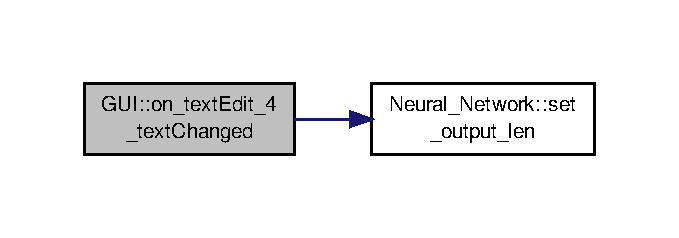
\includegraphics[width=326pt]{d7/d46/a00002_a39f58394bb8e9691a7b32774114a910a_cgraph}
\end{center}
\end{figure}


\hypertarget{a00002_ade6ba53055965b3522fa3cd022e4c5e0}{\index{G\-U\-I@{G\-U\-I}!perform\-\_\-test@{perform\-\_\-test}}
\index{perform\-\_\-test@{perform\-\_\-test}!GUI@{G\-U\-I}}
\subsubsection[{perform\-\_\-test}]{\setlength{\rightskip}{0pt plus 5cm}void G\-U\-I\-::perform\-\_\-test (
\begin{DoxyParamCaption}
{}
\end{DoxyParamCaption}
)\hspace{0.3cm}{\ttfamily [private]}}}\label{d7/d46/a00002_ade6ba53055965b3522fa3cd022e4c5e0}

\begin{DoxyParams}{Parameters}
{\em Calls} & file manager rotines to test.\par

\begin{DoxyEnumerate}
\item read input.\par

\item read weights.\par

\item test.\par

\item write output.\par
 
\end{DoxyEnumerate}\\
\hline
\end{DoxyParams}


Definition at line 60 of file G\-U\-I\-\_\-start\-Button.\-cpp.



References Neural\-\_\-\-Network\-::do\-\_\-function(), File\-\_\-\-Manager\-::do\-\_\-function(), fm, File\-\_\-\-Manager\-::get\-\_\-input\-\_\-population\-\_\-string(), File\-\_\-\-Manager\-::get\-\_\-output\-\_\-population\-\_\-string(), File\-\_\-\-Manager\-::n, and ui.



Here is the call graph for this function\-:\nopagebreak
\begin{figure}[H]
\begin{center}
\leavevmode
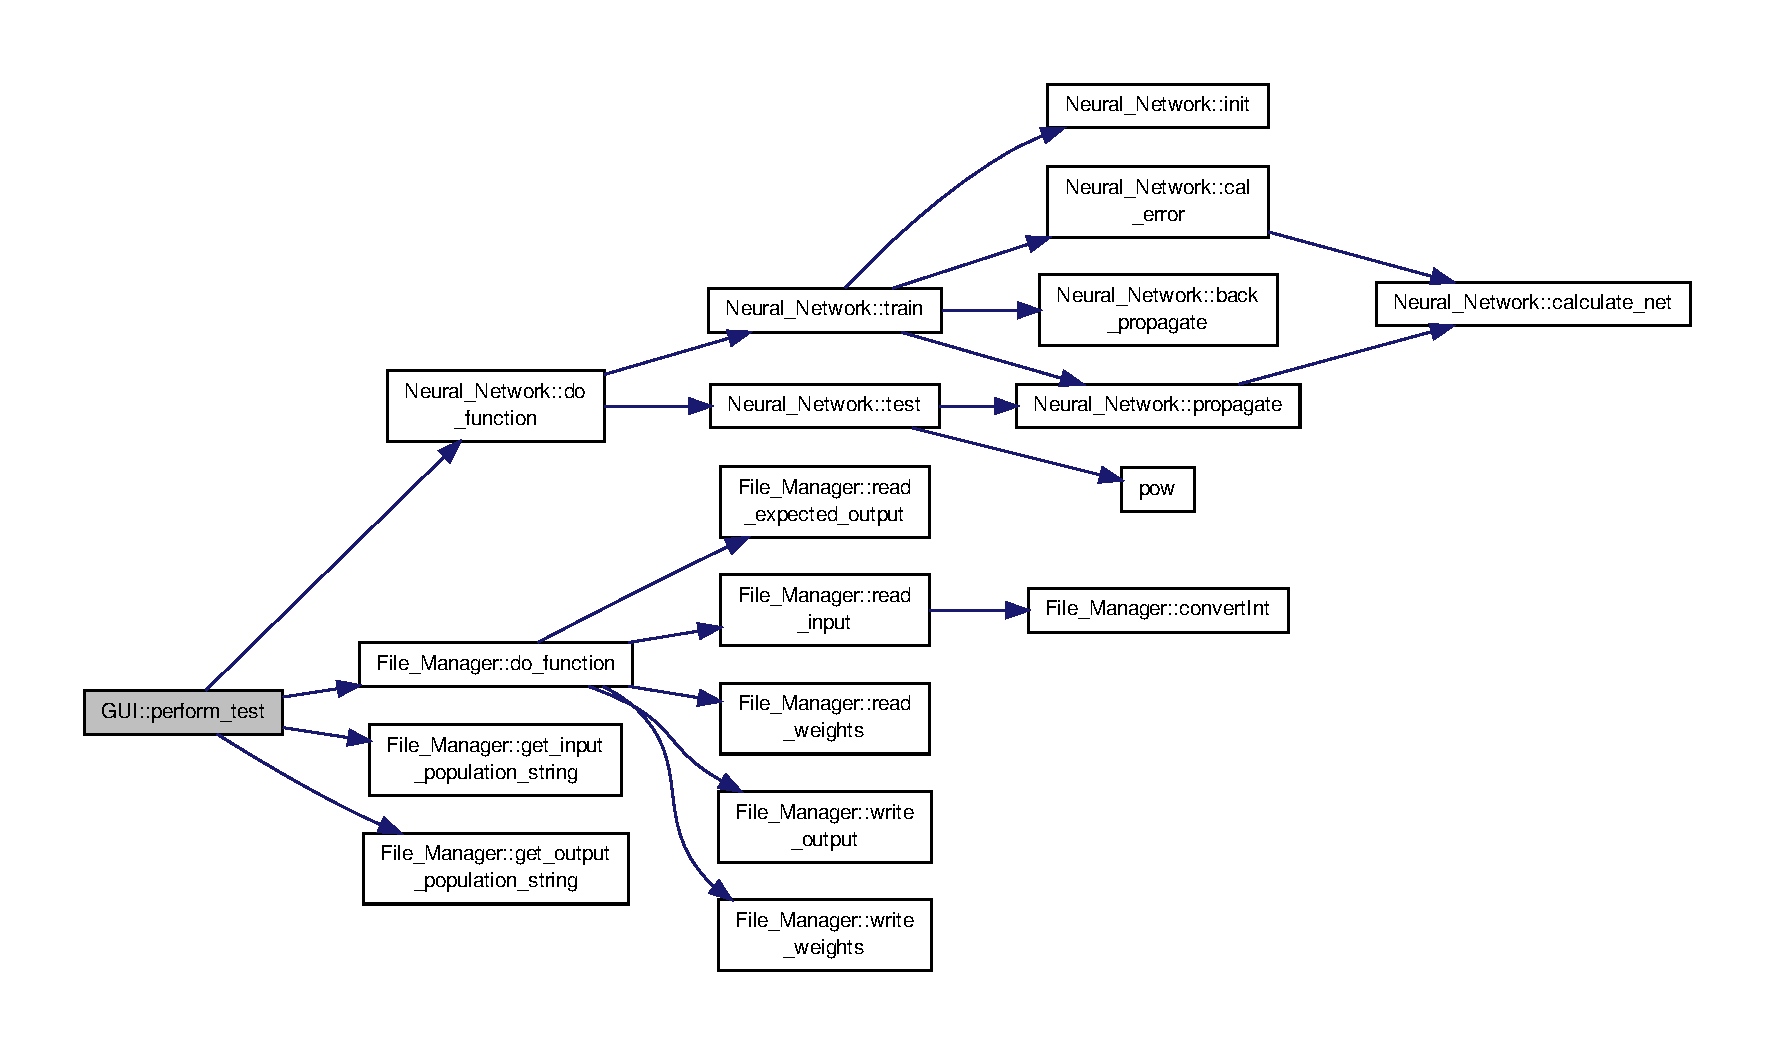
\includegraphics[width=350pt]{d7/d46/a00002_ade6ba53055965b3522fa3cd022e4c5e0_cgraph}
\end{center}
\end{figure}




Here is the caller graph for this function\-:\nopagebreak
\begin{figure}[H]
\begin{center}
\leavevmode
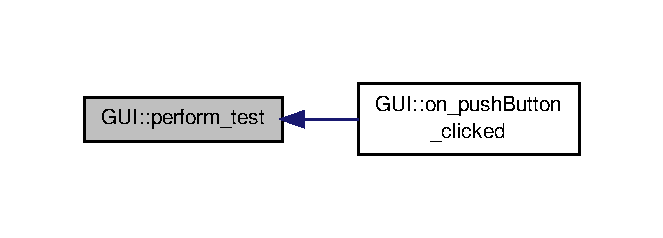
\includegraphics[width=318pt]{d7/d46/a00002_ade6ba53055965b3522fa3cd022e4c5e0_icgraph}
\end{center}
\end{figure}


\hypertarget{a00002_ad1bb069dee02010a61045c91f5e7752f}{\index{G\-U\-I@{G\-U\-I}!perform\-\_\-train@{perform\-\_\-train}}
\index{perform\-\_\-train@{perform\-\_\-train}!GUI@{G\-U\-I}}
\subsubsection[{perform\-\_\-train}]{\setlength{\rightskip}{0pt plus 5cm}void G\-U\-I\-::perform\-\_\-train (
\begin{DoxyParamCaption}
{}
\end{DoxyParamCaption}
)\hspace{0.3cm}{\ttfamily [private]}}}\label{d7/d46/a00002_ad1bb069dee02010a61045c91f5e7752f}


Calls file manager rotines to train\-:\par
. 


\begin{DoxyEnumerate}
\item read input.\par

\item read expected output.\par

\item train.\par

\item write weights. 
\end{DoxyEnumerate}

Definition at line 35 of file G\-U\-I\-\_\-start\-Button.\-cpp.



References Neural\-\_\-\-Network\-::do\-\_\-function(), File\-\_\-\-Manager\-::do\-\_\-function(), fm, File\-\_\-\-Manager\-::get\-\_\-input\-\_\-population\-\_\-string(), File\-\_\-\-Manager\-::get\-\_\-read\-\_\-ex\-\_\-output\-\_\-string(), File\-\_\-\-Manager\-::n, and ui.



Here is the call graph for this function\-:\nopagebreak
\begin{figure}[H]
\begin{center}
\leavevmode
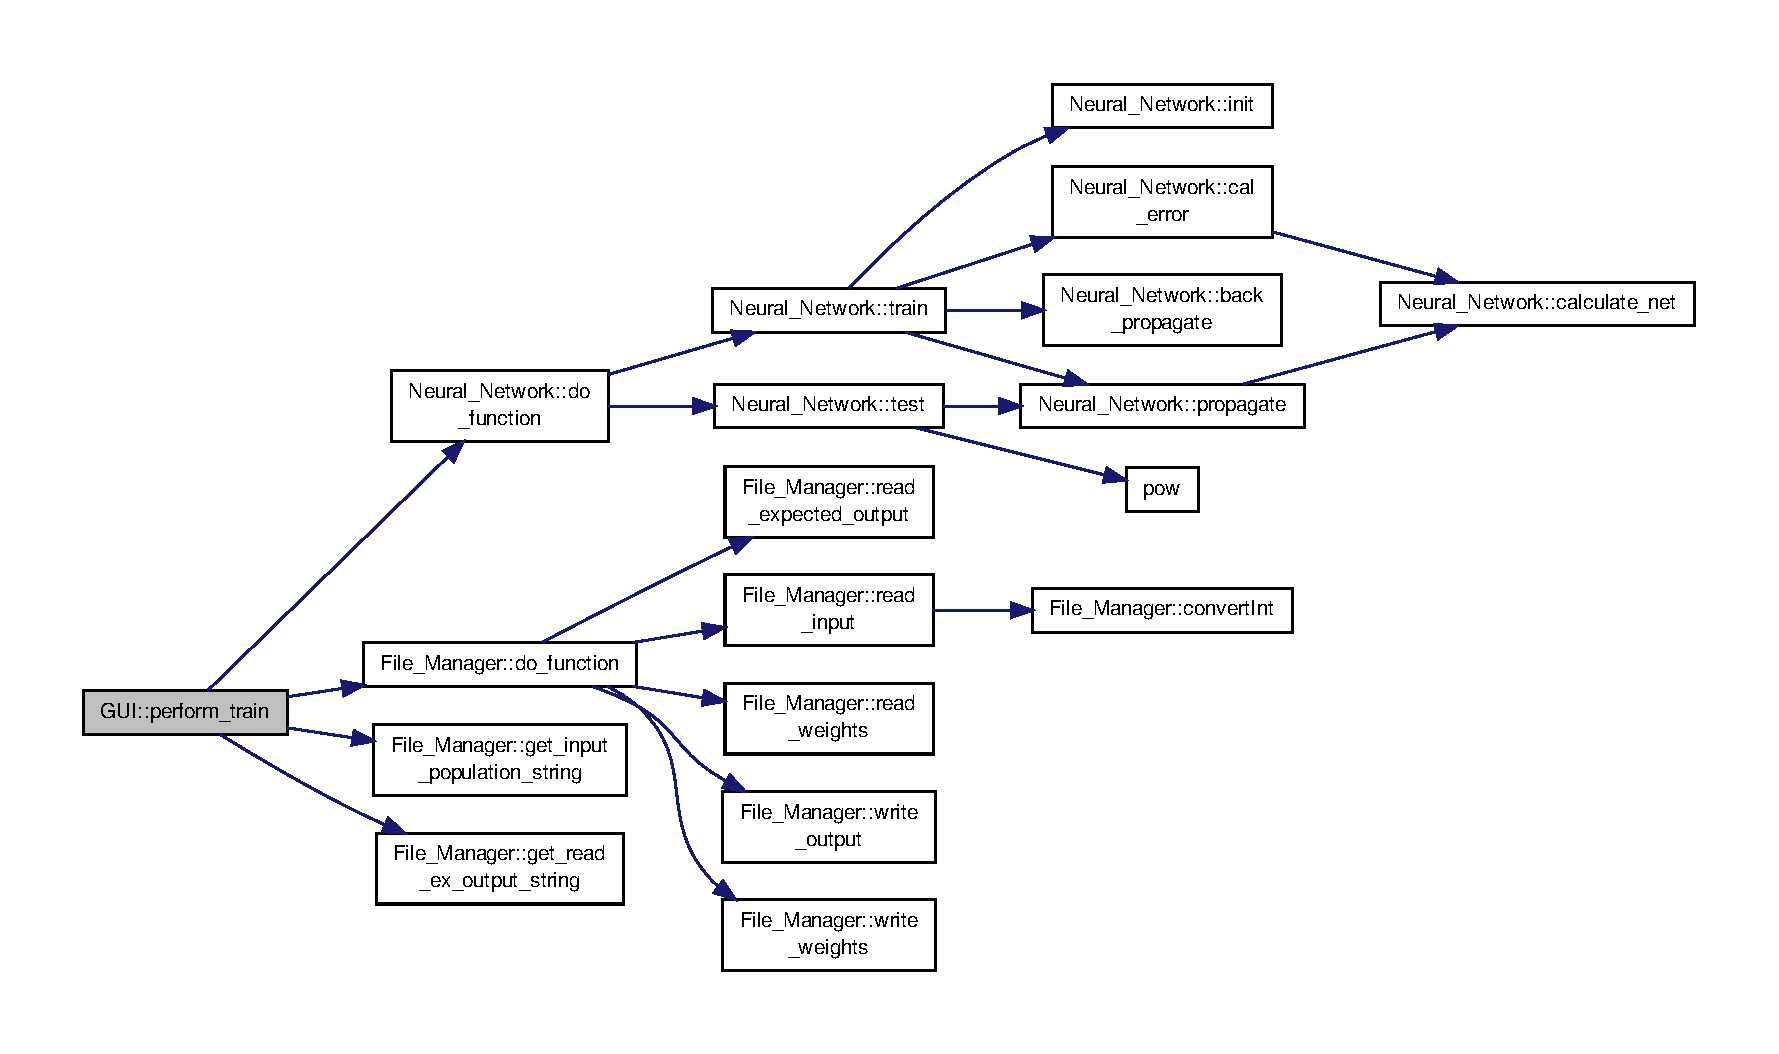
\includegraphics[width=350pt]{d7/d46/a00002_ad1bb069dee02010a61045c91f5e7752f_cgraph}
\end{center}
\end{figure}




Here is the caller graph for this function\-:\nopagebreak
\begin{figure}[H]
\begin{center}
\leavevmode
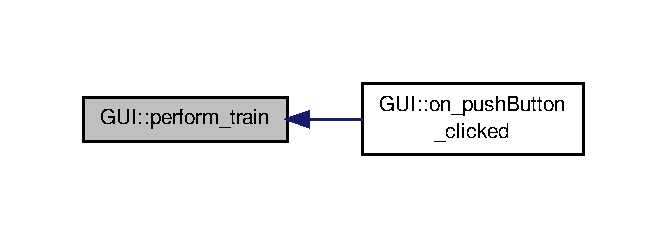
\includegraphics[width=320pt]{d7/d46/a00002_ad1bb069dee02010a61045c91f5e7752f_icgraph}
\end{center}
\end{figure}


\hypertarget{a00002_a5683a1862ec1a85cf87d9c5f6fc528e9}{\index{G\-U\-I@{G\-U\-I}!set\-\_\-style\-Sheet@{set\-\_\-style\-Sheet}}
\index{set\-\_\-style\-Sheet@{set\-\_\-style\-Sheet}!GUI@{G\-U\-I}}
\subsubsection[{set\-\_\-style\-Sheet}]{\setlength{\rightskip}{0pt plus 5cm}void G\-U\-I\-::set\-\_\-style\-Sheet (
\begin{DoxyParamCaption}
{}
\end{DoxyParamCaption}
)\hspace{0.3cm}{\ttfamily [private]}}}\label{d7/d46/a00002_a5683a1862ec1a85cf87d9c5f6fc528e9}


Set style sheet configuration\-: Set color grey for some labels. 



Definition at line 20 of file G\-U\-I\-\_\-constructor.\-cpp.



References ui.



Here is the caller graph for this function\-:\nopagebreak
\begin{figure}[H]
\begin{center}
\leavevmode
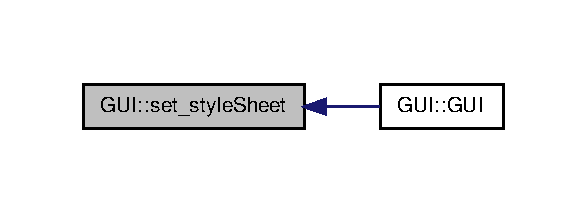
\includegraphics[width=282pt]{d7/d46/a00002_a5683a1862ec1a85cf87d9c5f6fc528e9_icgraph}
\end{center}
\end{figure}


\hypertarget{a00002_abd9fac4d8ad5334cc48afb0513544898}{\index{G\-U\-I@{G\-U\-I}!set\-\_\-validators@{set\-\_\-validators}}
\index{set\-\_\-validators@{set\-\_\-validators}!GUI@{G\-U\-I}}
\subsubsection[{set\-\_\-validators}]{\setlength{\rightskip}{0pt plus 5cm}void G\-U\-I\-::set\-\_\-validators (
\begin{DoxyParamCaption}
{}
\end{DoxyParamCaption}
)\hspace{0.3cm}{\ttfamily [private]}}}\label{d7/d46/a00002_abd9fac4d8ad5334cc48afb0513544898}


Set validators for user input. 



Definition at line 31 of file G\-U\-I\-\_\-constructor.\-cpp.



References ui.



Here is the caller graph for this function\-:\nopagebreak
\begin{figure}[H]
\begin{center}
\leavevmode
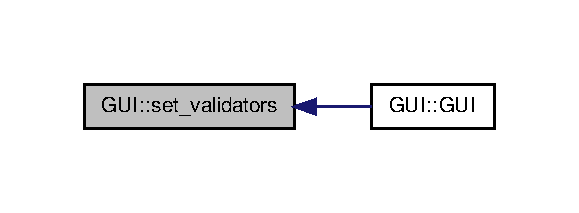
\includegraphics[width=278pt]{d7/d46/a00002_abd9fac4d8ad5334cc48afb0513544898_icgraph}
\end{center}
\end{figure}


\hypertarget{a00002_a5ec9d8a051303b218c4542f96a87b56f}{\index{G\-U\-I@{G\-U\-I}!valid\-\_\-input@{valid\-\_\-input}}
\index{valid\-\_\-input@{valid\-\_\-input}!GUI@{G\-U\-I}}
\subsubsection[{valid\-\_\-input}]{\setlength{\rightskip}{0pt plus 5cm}Q\-String G\-U\-I\-::valid\-\_\-input (
\begin{DoxyParamCaption}
{}
\end{DoxyParamCaption}
)\hspace{0.3cm}{\ttfamily [private]}}}\label{d7/d46/a00002_a5ec9d8a051303b218c4542f96a87b56f}


Check that all input needed is filled. 



Definition at line 79 of file G\-U\-I\-\_\-start\-Button.\-cpp.



References fill\-\_\-rank(), fm, fori, Neural\-\_\-\-Network\-::get\-\_\-output\-\_\-len(), File\-\_\-\-Manager\-::get\-\_\-rank\-\_\-output\-\_\-strings(), File\-\_\-\-Manager\-::n, and ui.



Here is the call graph for this function\-:
\nopagebreak
\begin{figure}[H]
\begin{center}
\leavevmode
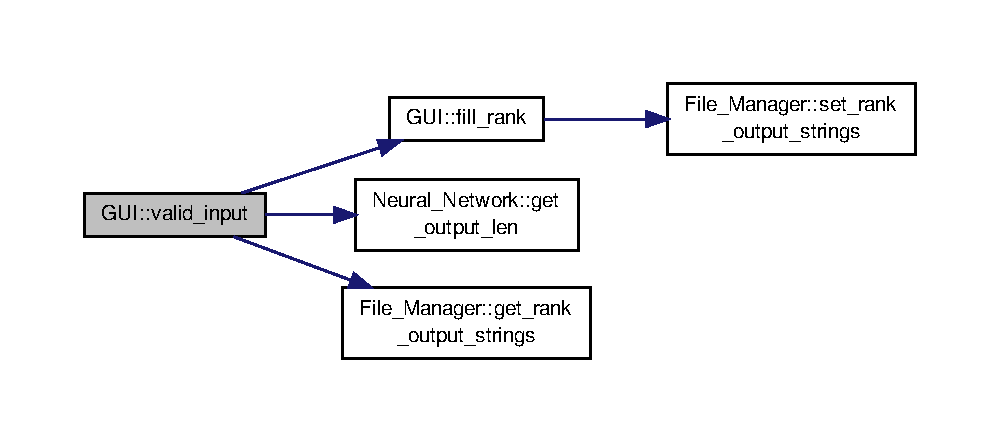
\includegraphics[width=350pt]{d7/d46/a00002_a5ec9d8a051303b218c4542f96a87b56f_cgraph}
\end{center}
\end{figure}




Here is the caller graph for this function\-:\nopagebreak
\begin{figure}[H]
\begin{center}
\leavevmode
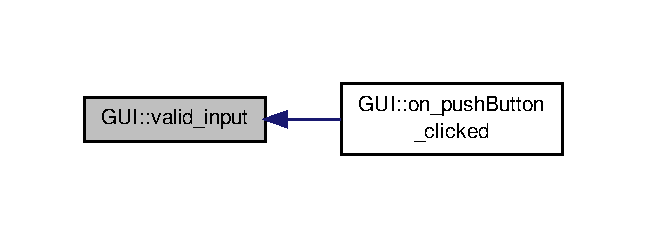
\includegraphics[width=310pt]{d7/d46/a00002_a5ec9d8a051303b218c4542f96a87b56f_icgraph}
\end{center}
\end{figure}




\subsection{Member Data Documentation}
\hypertarget{a00002_a9ed0a8b583419e88bb94697a9b258c72}{\index{G\-U\-I@{G\-U\-I}!file\-Dialog@{file\-Dialog}}
\index{file\-Dialog@{file\-Dialog}!GUI@{G\-U\-I}}
\subsubsection[{file\-Dialog}]{\setlength{\rightskip}{0pt plus 5cm}Q\-File\-Dialog G\-U\-I\-::file\-Dialog\hspace{0.3cm}{\ttfamily [private]}}}\label{d7/d46/a00002_a9ed0a8b583419e88bb94697a9b258c72}


Definition at line 21 of file G\-U\-I.\-h.

\hypertarget{a00002_a62d0a4c604ed8d65f85455971a938548}{\index{G\-U\-I@{G\-U\-I}!file\-Path@{file\-Path}}
\index{file\-Path@{file\-Path}!GUI@{G\-U\-I}}
\subsubsection[{file\-Path}]{\setlength{\rightskip}{0pt plus 5cm}Q\-String G\-U\-I\-::file\-Path\hspace{0.3cm}{\ttfamily [private]}}}\label{d7/d46/a00002_a62d0a4c604ed8d65f85455971a938548}


Definition at line 20 of file G\-U\-I.\-h.

\hypertarget{a00002_a73cc90505024488d2fd77762ad5059c4}{\index{G\-U\-I@{G\-U\-I}!fm@{fm}}
\index{fm@{fm}!GUI@{G\-U\-I}}
\subsubsection[{fm}]{\setlength{\rightskip}{0pt plus 5cm}{\bf File\-\_\-\-Manager} G\-U\-I\-::fm\hspace{0.3cm}{\ttfamily [private]}}}\label{d7/d46/a00002_a73cc90505024488d2fd77762ad5059c4}


Definition at line 45 of file G\-U\-I.\-h.

\hypertarget{a00002_aa3abed87f53b22188d76a134e427b30d}{\index{G\-U\-I@{G\-U\-I}!state@{state}}
\index{state@{state}!GUI@{G\-U\-I}}
\subsubsection[{state}]{\setlength{\rightskip}{0pt plus 5cm}Q\-Byte\-Array G\-U\-I\-::state\hspace{0.3cm}{\ttfamily [private]}}}\label{d7/d46/a00002_aa3abed87f53b22188d76a134e427b30d}


Definition at line 22 of file G\-U\-I.\-h.

\hypertarget{a00002_acdbca1224663f5a19bd1ad4e7c885886}{\index{G\-U\-I@{G\-U\-I}!ui@{ui}}
\index{ui@{ui}!GUI@{G\-U\-I}}
\subsubsection[{ui}]{\setlength{\rightskip}{0pt plus 5cm}Ui\-::\-G\-U\-I$\ast$ G\-U\-I\-::ui\hspace{0.3cm}{\ttfamily [private]}}}\label{d7/d46/a00002_acdbca1224663f5a19bd1ad4e7c885886}


Definition at line 43 of file G\-U\-I.\-h.



The documentation for this class was generated from the following files\-:\begin{DoxyCompactItemize}
\item 
phenogene/\hyperlink{a00010}{G\-U\-I.\-h}\item 
phenogene/\hyperlink{a00009}{G\-U\-I.\-cpp}\item 
phenogene/\hyperlink{a00011}{G\-U\-I\-\_\-constructor.\-cpp}\item 
phenogene/\hyperlink{a00012}{G\-U\-I\-\_\-start\-Button.\-cpp}\end{DoxyCompactItemize}

\hypertarget{a00003}{\section{Neural\-\_\-\-Network Class Reference}
\label{d1/d7c/a00003}\index{Neural\-\_\-\-Network@{Neural\-\_\-\-Network}}
}


{\ttfamily \#include $<$Neural\-Network.\-h$>$}



Collaboration diagram for Neural\-\_\-\-Network\-:\nopagebreak
\begin{figure}[H]
\begin{center}
\leavevmode
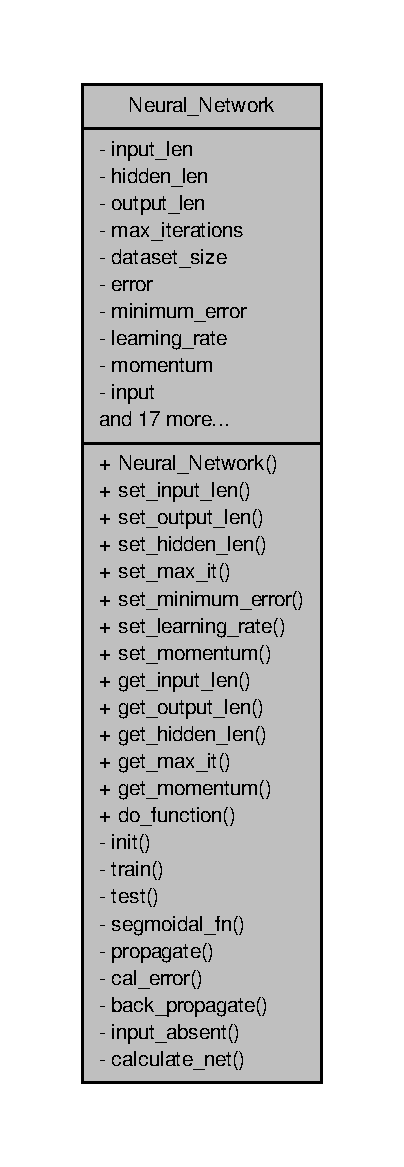
\includegraphics[width=194pt]{d3/dea/a00046}
\end{center}
\end{figure}
\subsection*{Public Member Functions}
\begin{DoxyCompactItemize}
\item 
\hyperlink{a00003_a6f3defa930afbcb64a305393f741a2a4}{Neural\-\_\-\-Network} ()
\begin{DoxyCompactList}\small\item\em Neural Network class constructor. \end{DoxyCompactList}\item 
void \hyperlink{a00003_afb37f8321b35bbc9b9beb88d56d69f08}{set\-\_\-input\-\_\-len} (int)
\begin{DoxyCompactList}\small\item\em Set number of input nodes to int i. \end{DoxyCompactList}\item 
void \hyperlink{a00003_a695079279950a3eb27d62df68d32927c}{set\-\_\-output\-\_\-len} (int)
\begin{DoxyCompactList}\small\item\em Set number of output to int i. \end{DoxyCompactList}\item 
void \hyperlink{a00003_ad1e1afff306e47947e23f4fdd4517e22}{set\-\_\-hidden\-\_\-len} (int)
\begin{DoxyCompactList}\small\item\em Set hidden nodes to int i. \end{DoxyCompactList}\item 
void \hyperlink{a00003_a80b2c577da9fdc4e830722e7a4569069}{set\-\_\-\-A\-V} (int)
\begin{DoxyCompactList}\small\item\em Set Activation function to be used to int i. \end{DoxyCompactList}\item 
void \hyperlink{a00003_a0458bfedabe1b42e4d30e3179bd1f189}{set\-\_\-minimum\-\_\-error} (double)
\begin{DoxyCompactList}\small\item\em Set minimum error to double d. \end{DoxyCompactList}\item 
void \hyperlink{a00003_a87a3c876501fcd89ffc1caf298fa2703}{set\-\_\-learning\-\_\-rate} (double)
\begin{DoxyCompactList}\small\item\em Set learning rate to double d. \end{DoxyCompactList}\item 
int \hyperlink{a00003_a75e25e607afb4e862219b21c0569c893}{get\-\_\-input\-\_\-len} ()
\begin{DoxyCompactList}\small\item\em Get int number of input nodes. \end{DoxyCompactList}\item 
int \hyperlink{a00003_a895c1b35110b7ee5e5adc56a63a55e78}{get\-\_\-output\-\_\-len} ()
\begin{DoxyCompactList}\small\item\em Get int number of output nodes. \end{DoxyCompactList}\item 
int \hyperlink{a00003_ac781308fb521309d657b91a95054be52}{get\-\_\-hidden\-\_\-len} ()
\begin{DoxyCompactList}\small\item\em Get int number of hidden nodes. \end{DoxyCompactList}\item 
void \hyperlink{a00003_acd3d4762d71d54422b45fda3a13976cf}{do\-\_\-function} (int)
\begin{DoxyCompactList}\small\item\em Train or test the network. \end{DoxyCompactList}\end{DoxyCompactItemize}
\subsection*{Private Member Functions}
\begin{DoxyCompactItemize}
\item 
void \hyperlink{a00003_ac86567c994bb671c20ed50316d268d3b}{init} ()
\begin{DoxyCompactList}\small\item\em Initialize weights and biases with values between -\/0.\-5 and 0.\-5. \end{DoxyCompactList}\item 
void \hyperlink{a00003_a033f4f60812c0359cc50815e957f11f7}{train} ()
\begin{DoxyCompactList}\small\item\em Train the neural network\-: \end{DoxyCompactList}\item 
void \hyperlink{a00003_a38193cc61e9affbd077c1c6089fd0889}{test} ()
\begin{DoxyCompactList}\small\item\em Test the neural network. \end{DoxyCompactList}\item 
double \hyperlink{a00003_a7a8eff736645e4101ed906a46e6a27ac}{segmoidal\-\_\-fn} (double, int)
\begin{DoxyCompactList}\small\item\em Calculates the segmoidal/segmoidal inverse of a double \mbox{[}x\mbox{]}. \end{DoxyCompactList}\item 
void \hyperlink{a00003_a7e6d776ecfbb4f9df682d5fe13a7ec3b}{propagate} ()
\begin{DoxyCompactList}\small\item\em Propagate input starting from the input layer up to the output layer. Uses softmax activation function. \end{DoxyCompactList}\item 
double \hyperlink{a00003_a3e503ddab5bbc51f6e0b79b67ca6ed2f}{cal\-\_\-error} ()
\begin{DoxyCompactList}\small\item\em Calculate the error signal for each node. Uses corss entropy error function. \end{DoxyCompactList}\item 
void \hyperlink{a00003_a5a0cac77d13e3ffdd3088cb684d39859}{back\-\_\-propagate} ()
\begin{DoxyCompactList}\small\item\em Back propagate the error starting from the output layer down to the input layer. \end{DoxyCompactList}\item 
bool \hyperlink{a00003_a3d073d4957def9b6a4498448260fedeb}{input\-\_\-absent} ()
\item 
void \hyperlink{a00003_a25df8564c3f26b64935464366055572e}{calculate\-\_\-net} (double \&, double \&)
\begin{DoxyCompactList}\small\item\em Calculates the net for each node. \end{DoxyCompactList}\end{DoxyCompactItemize}
\subsection*{Private Attributes}
\begin{DoxyCompactItemize}
\item 
int \hyperlink{a00003_a9e5319bf385fa55bbbd8f0160915306d}{input\-\_\-len}
\item 
int \hyperlink{a00003_a71cc8ca03da47fe639dd1e8ed518069c}{hidden\-\_\-len}
\item 
int \hyperlink{a00003_a053d2b510e07b1f25ef112f366bc62ba}{output\-\_\-len}
\item 
int \hyperlink{a00003_a970136042929b26220d35be2776220a6}{A\-V}
\item 
int \hyperlink{a00003_a8fe39196b36a38696abd679328dd8232}{dataset\-\_\-size}
\item 
double \hyperlink{a00003_a2ffe42aee798e268d4bbf0f3428ba430}{error}
\item 
double \hyperlink{a00003_aa2898d2ec7ac091b6d40916d4b113a93}{minimum\-\_\-error}
\item 
double \hyperlink{a00003_a1994986029a1ef9d55fa4bb1b440210b}{learning\-\_\-rate}
\item 
double \hyperlink{a00003_a3a3ea713384da26e538bc60da8410a75}{momentum}
\item 
double \hyperlink{a00003_a347a1fceb1ac048ecd913a89126cebb3}{input} \mbox{[}\hyperlink{a00008_a8dae3b2c955083e02ba56da92adbf25d}{input\-\_\-l}\mbox{]}
\item 
double \hyperlink{a00003_a5b31deacdc5c63e687d6ebc086b761ab}{hidden} \mbox{[}\hyperlink{a00008_aa7fdf42e8c0a65ea15cb37a990708e36}{hidden\-\_\-l}\mbox{]}
\item 
double \hyperlink{a00003_abe5631cce6141b7756154a5a9d247da2}{output} \mbox{[}\hyperlink{a00008_a0a0ddfc9fb3bc3d90d175ed1f7bd54c5}{output\-\_\-l}\mbox{]}
\item 
double \hyperlink{a00003_aa07e5b1f8997f895d7550495a5b4f0d2}{net\-H} \mbox{[}\hyperlink{a00008_aa7fdf42e8c0a65ea15cb37a990708e36}{hidden\-\_\-l}\mbox{]}
\item 
double \hyperlink{a00003_a8bcf19afde3c08afbd862759c839a769}{net\-O} \mbox{[}\hyperlink{a00008_a0a0ddfc9fb3bc3d90d175ed1f7bd54c5}{output\-\_\-l}\mbox{]}
\item 
double \hyperlink{a00003_a8d632cf69d2fcd076e473aba1ae74702}{expected\-\_\-o} \mbox{[}\hyperlink{a00008_a0a0ddfc9fb3bc3d90d175ed1f7bd54c5}{output\-\_\-l}\mbox{]}
\item 
double \hyperlink{a00003_a8f26363ac0ccda6f04df35e68164cd3a}{bias\-\_\-\-O} \mbox{[}\hyperlink{a00008_a0a0ddfc9fb3bc3d90d175ed1f7bd54c5}{output\-\_\-l}\mbox{]}
\item 
double \hyperlink{a00003_a38808438a02d406a7ab54c8bf825752a}{bias\-\_\-\-H} \mbox{[}\hyperlink{a00008_aa7fdf42e8c0a65ea15cb37a990708e36}{hidden\-\_\-l}\mbox{]}
\item 
double \hyperlink{a00003_a45dfc138d645e05eaeaa6ca6bb3df818}{Wh} \mbox{[}\hyperlink{a00008_aa7fdf42e8c0a65ea15cb37a990708e36}{hidden\-\_\-l}\mbox{]}\mbox{[}\hyperlink{a00008_a8dae3b2c955083e02ba56da92adbf25d}{input\-\_\-l}\mbox{]}
\item 
double \hyperlink{a00003_ad6730ce7c9fc3937299dd32473b12d1d}{Wo} \mbox{[}\hyperlink{a00008_a0a0ddfc9fb3bc3d90d175ed1f7bd54c5}{output\-\_\-l}\mbox{]}\mbox{[}\hyperlink{a00008_aa7fdf42e8c0a65ea15cb37a990708e36}{hidden\-\_\-l}\mbox{]}
\item 
double \hyperlink{a00003_a1cca3513af05c6dce603fdf332b36691}{temp\-Wo} \mbox{[}\hyperlink{a00008_a0a0ddfc9fb3bc3d90d175ed1f7bd54c5}{output\-\_\-l}\mbox{]}\mbox{[}\hyperlink{a00008_aa7fdf42e8c0a65ea15cb37a990708e36}{hidden\-\_\-l}\mbox{]}
\item 
double \hyperlink{a00003_ae5f829ba5e65ae91d5c4feda5f66e37a}{delta\-\_\-\-O} \mbox{[}\hyperlink{a00008_a0a0ddfc9fb3bc3d90d175ed1f7bd54c5}{output\-\_\-l}\mbox{]}
\item 
double \hyperlink{a00003_a51e5c2d2b53ba284c5b3791446c3b7d8}{delta\-\_\-\-H} \mbox{[}\hyperlink{a00008_aa7fdf42e8c0a65ea15cb37a990708e36}{hidden\-\_\-l}\mbox{]}
\item 
map$<$ char, double $>$ \hyperlink{a00003_adf2c6662b130ed1582025ea2cccacbe2}{input\-\_\-rank}
\item 
map$<$ string, int $>$ \hyperlink{a00003_af46a9de8ef619f93fb8c0231be79163c}{output\-\_\-rank}
\item 
map$<$ int, string $>$ \hyperlink{a00003_a8e34531b701290d16068e3685f3066a4}{rank\-\_\-output}
\item 
vector$<$ vector$<$ double $>$ $>$ \hyperlink{a00003_a81bab51b36643c5b10ba25d518c27ff3}{input\-\_\-dataset}
\item 
vector$<$ vector$<$ double $>$ $>$ \hyperlink{a00003_aa8441449f55f07c3da384d81608373b5}{output\-\_\-dataset}
\end{DoxyCompactItemize}
\subsection*{Friends}
\begin{DoxyCompactItemize}
\item 
class \hyperlink{a00003_a96aa84fcda6b19a74fff9d19c16b07fe}{File\-\_\-\-Manager}
\end{DoxyCompactItemize}


\subsection{Detailed Description}


Definition at line 6 of file Neural\-Network.\-h.



\subsection{Constructor \& Destructor Documentation}
\hypertarget{a00003_a6f3defa930afbcb64a305393f741a2a4}{\index{Neural\-\_\-\-Network@{Neural\-\_\-\-Network}!Neural\-\_\-\-Network@{Neural\-\_\-\-Network}}
\index{Neural\-\_\-\-Network@{Neural\-\_\-\-Network}!Neural_Network@{Neural\-\_\-\-Network}}
\subsubsection[{Neural\-\_\-\-Network}]{\setlength{\rightskip}{0pt plus 5cm}Neural\-\_\-\-Network\-::\-Neural\-\_\-\-Network (
\begin{DoxyParamCaption}
{}
\end{DoxyParamCaption}
)}}\label{d1/d7c/a00003_a6f3defa930afbcb64a305393f741a2a4}


Neural Network class constructor. 



Definition at line 7 of file N\-N\-\_\-constructor.\-cpp.



References A\-V, dataset\-\_\-size, hidden\-\_\-len, input\-\_\-len, input\-\_\-rank, learning\-\_\-rate, minimum\-\_\-error, momentum, output\-\_\-len, and segmoidal.



\subsection{Member Function Documentation}
\hypertarget{a00003_a5a0cac77d13e3ffdd3088cb684d39859}{\index{Neural\-\_\-\-Network@{Neural\-\_\-\-Network}!back\-\_\-propagate@{back\-\_\-propagate}}
\index{back\-\_\-propagate@{back\-\_\-propagate}!Neural_Network@{Neural\-\_\-\-Network}}
\subsubsection[{back\-\_\-propagate}]{\setlength{\rightskip}{0pt plus 5cm}void Neural\-\_\-\-Network\-::back\-\_\-propagate (
\begin{DoxyParamCaption}
{}
\end{DoxyParamCaption}
)\hspace{0.3cm}{\ttfamily [private]}}}\label{d1/d7c/a00003_a5a0cac77d13e3ffdd3088cb684d39859}


Back propagate the error starting from the output layer down to the input layer. 

\begin{DoxyPrecond}{Precondition}
Delta signal for each node has been calculated. 

Bias and Weights doesn't hold garpage. 
\end{DoxyPrecond}
\begin{DoxyPostcond}{Postcondition}
Bias and Weights are updated. 
\end{DoxyPostcond}


Definition at line 211 of file N\-N.\-cpp.



References bias\-\_\-\-H, bias\-\_\-\-O, delta\-\_\-\-H, delta\-\_\-\-O, fori, forj, hidden, hidden\-\_\-len, input, input\-\_\-len, learning\-\_\-rate, momentum, output\-\_\-len, Wh, and Wo.



Here is the caller graph for this function\-:
\nopagebreak
\begin{figure}[H]
\begin{center}
\leavevmode
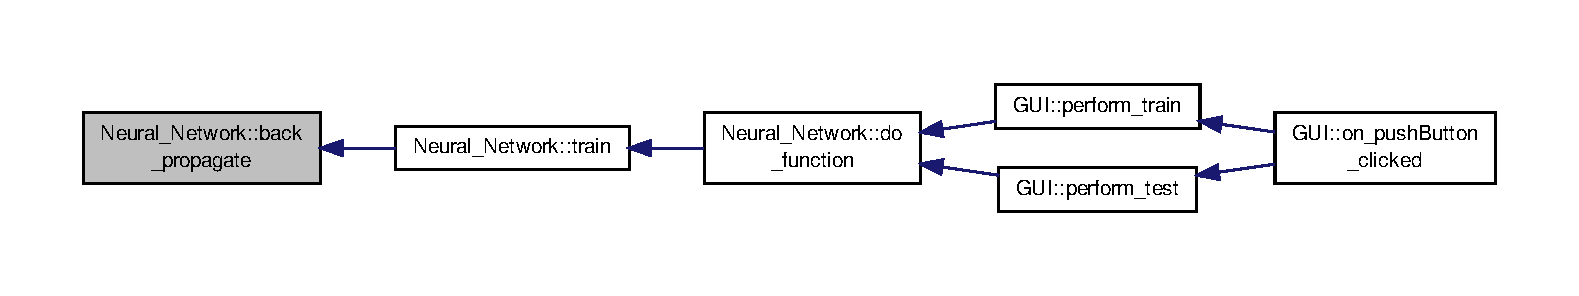
\includegraphics[width=350pt]{d1/d7c/a00003_a5a0cac77d13e3ffdd3088cb684d39859_icgraph}
\end{center}
\end{figure}


\hypertarget{a00003_a3e503ddab5bbc51f6e0b79b67ca6ed2f}{\index{Neural\-\_\-\-Network@{Neural\-\_\-\-Network}!cal\-\_\-error@{cal\-\_\-error}}
\index{cal\-\_\-error@{cal\-\_\-error}!Neural_Network@{Neural\-\_\-\-Network}}
\subsubsection[{cal\-\_\-error}]{\setlength{\rightskip}{0pt plus 5cm}double Neural\-\_\-\-Network\-::cal\-\_\-error (
\begin{DoxyParamCaption}
{}
\end{DoxyParamCaption}
)\hspace{0.3cm}{\ttfamily [private]}}}\label{d1/d7c/a00003_a3e503ddab5bbc51f6e0b79b67ca6ed2f}


Calculate the error signal for each node. Uses corss entropy error function. 

\begin{DoxyReturn}{Returns}
\mbox{[}total error\mbox{]} 
\end{DoxyReturn}
\begin{DoxyPrecond}{Precondition}
Actual output is calculated using function \mbox{[}propagate\mbox{]}. 
\end{DoxyPrecond}
\begin{DoxyPostcond}{Postcondition}
Delta signal for all nodes is calculated. 
\end{DoxyPostcond}


Definition at line 239 of file N\-N.\-cpp.



References calculate\-\_\-net(), delta\-\_\-\-H, delta\-\_\-\-O, expected\-\_\-o, fori, forj, hidden\-\_\-len, net\-H, net\-O, output, and output\-\_\-len.



Here is the call graph for this function\-:\nopagebreak
\begin{figure}[H]
\begin{center}
\leavevmode
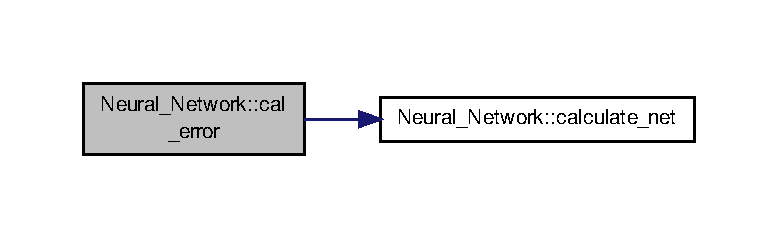
\includegraphics[width=350pt]{d1/d7c/a00003_a3e503ddab5bbc51f6e0b79b67ca6ed2f_cgraph}
\end{center}
\end{figure}




Here is the caller graph for this function\-:
\nopagebreak
\begin{figure}[H]
\begin{center}
\leavevmode
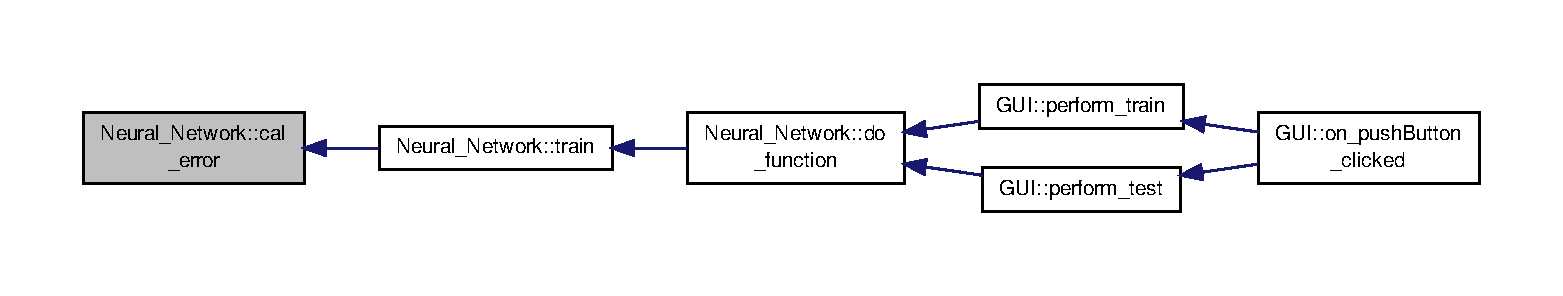
\includegraphics[width=350pt]{d1/d7c/a00003_a3e503ddab5bbc51f6e0b79b67ca6ed2f_icgraph}
\end{center}
\end{figure}


\hypertarget{a00003_a25df8564c3f26b64935464366055572e}{\index{Neural\-\_\-\-Network@{Neural\-\_\-\-Network}!calculate\-\_\-net@{calculate\-\_\-net}}
\index{calculate\-\_\-net@{calculate\-\_\-net}!Neural_Network@{Neural\-\_\-\-Network}}
\subsubsection[{calculate\-\_\-net}]{\setlength{\rightskip}{0pt plus 5cm}void Neural\-\_\-\-Network\-::calculate\-\_\-net (
\begin{DoxyParamCaption}
\item[{double \&}]{max, }
\item[{double \&}]{max\-O}
\end{DoxyParamCaption}
)\hspace{0.3cm}{\ttfamily [private]}}}\label{d1/d7c/a00003_a25df8564c3f26b64935464366055572e}


Calculates the net for each node. 

\begin{DoxyPrecond}{Precondition}
Input dataset is filled. 

Weights dataset is initialized. 
\end{DoxyPrecond}
\begin{DoxyPostcond}{Postcondition}
Net is caculated for Output and Hidden nodes. 
\end{DoxyPostcond}


Definition at line 274 of file N\-N.\-cpp.



References fori, forj, hidden\-\_\-len, input, input\-\_\-len, net\-H, net\-O, output\-\_\-len, Wh, and Wo.



Here is the caller graph for this function\-:
\nopagebreak
\begin{figure}[H]
\begin{center}
\leavevmode
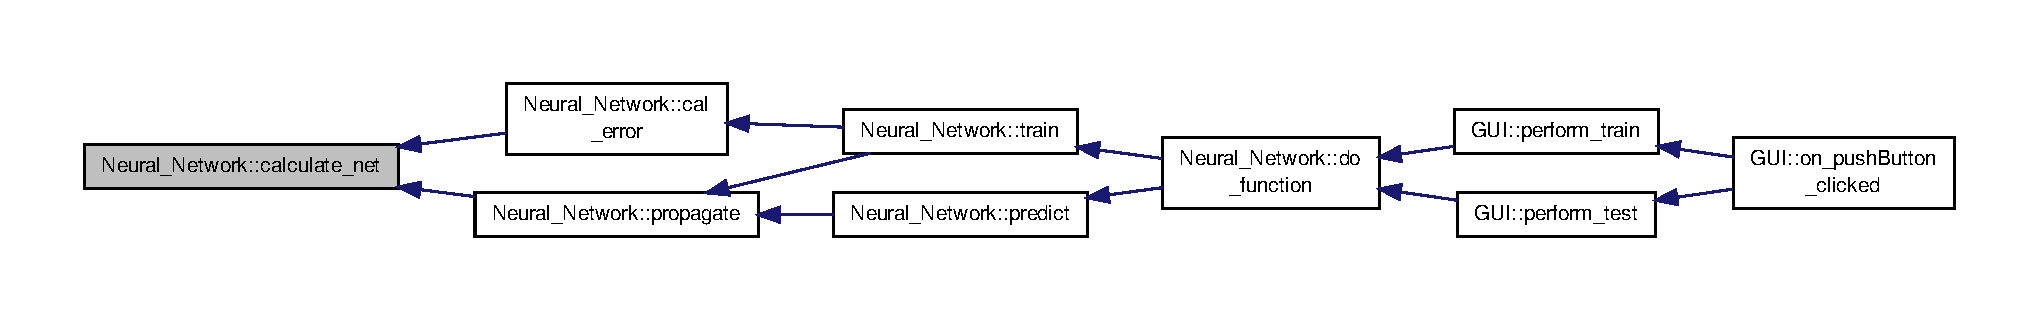
\includegraphics[width=350pt]{d1/d7c/a00003_a25df8564c3f26b64935464366055572e_icgraph}
\end{center}
\end{figure}


\hypertarget{a00003_acd3d4762d71d54422b45fda3a13976cf}{\index{Neural\-\_\-\-Network@{Neural\-\_\-\-Network}!do\-\_\-function@{do\-\_\-function}}
\index{do\-\_\-function@{do\-\_\-function}!Neural_Network@{Neural\-\_\-\-Network}}
\subsubsection[{do\-\_\-function}]{\setlength{\rightskip}{0pt plus 5cm}void Neural\-\_\-\-Network\-::do\-\_\-function (
\begin{DoxyParamCaption}
\item[{int}]{what}
\end{DoxyParamCaption}
)}}\label{d1/d7c/a00003_acd3d4762d71d54422b45fda3a13976cf}


Train or test the network. 


\begin{DoxyParams}{Parameters}
{\em \mbox{[}what\mbox{]}} & Determines weather to train or to test. \\
\hline
\end{DoxyParams}


Definition at line 7 of file N\-N.\-cpp.



References test(), and train().



Here is the call graph for this function\-:\nopagebreak
\begin{figure}[H]
\begin{center}
\leavevmode
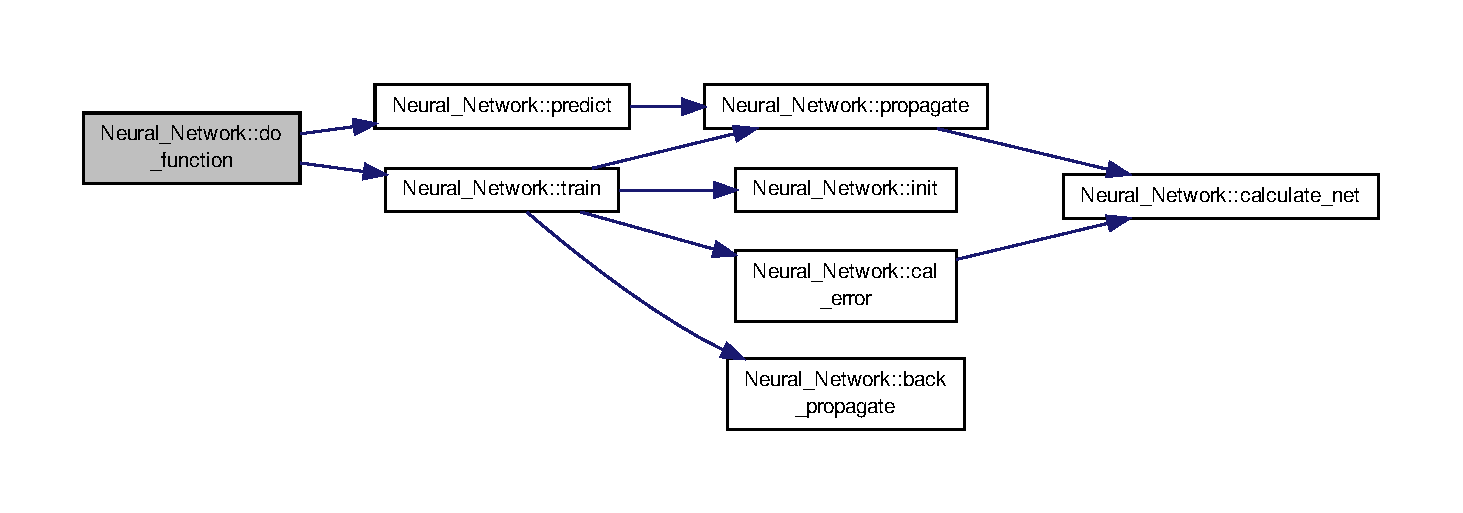
\includegraphics[width=350pt]{d1/d7c/a00003_acd3d4762d71d54422b45fda3a13976cf_cgraph}
\end{center}
\end{figure}




Here is the caller graph for this function\-:
\nopagebreak
\begin{figure}[H]
\begin{center}
\leavevmode
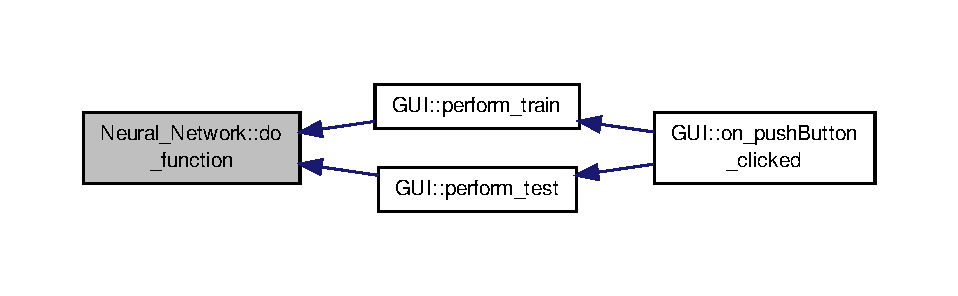
\includegraphics[width=350pt]{d1/d7c/a00003_acd3d4762d71d54422b45fda3a13976cf_icgraph}
\end{center}
\end{figure}


\hypertarget{a00003_ac781308fb521309d657b91a95054be52}{\index{Neural\-\_\-\-Network@{Neural\-\_\-\-Network}!get\-\_\-hidden\-\_\-len@{get\-\_\-hidden\-\_\-len}}
\index{get\-\_\-hidden\-\_\-len@{get\-\_\-hidden\-\_\-len}!Neural_Network@{Neural\-\_\-\-Network}}
\subsubsection[{get\-\_\-hidden\-\_\-len}]{\setlength{\rightskip}{0pt plus 5cm}int Neural\-\_\-\-Network\-::get\-\_\-hidden\-\_\-len (
\begin{DoxyParamCaption}
{}
\end{DoxyParamCaption}
)}}\label{d1/d7c/a00003_ac781308fb521309d657b91a95054be52}


Get int number of hidden nodes. 



Definition at line 24 of file N\-N\-\_\-getters.\-cpp.



References hidden\-\_\-len.

\hypertarget{a00003_a75e25e607afb4e862219b21c0569c893}{\index{Neural\-\_\-\-Network@{Neural\-\_\-\-Network}!get\-\_\-input\-\_\-len@{get\-\_\-input\-\_\-len}}
\index{get\-\_\-input\-\_\-len@{get\-\_\-input\-\_\-len}!Neural_Network@{Neural\-\_\-\-Network}}
\subsubsection[{get\-\_\-input\-\_\-len}]{\setlength{\rightskip}{0pt plus 5cm}int Neural\-\_\-\-Network\-::get\-\_\-input\-\_\-len (
\begin{DoxyParamCaption}
{}
\end{DoxyParamCaption}
)}}\label{d1/d7c/a00003_a75e25e607afb4e862219b21c0569c893}


Get int number of input nodes. 



Definition at line 6 of file N\-N\-\_\-getters.\-cpp.



References input\-\_\-len.

\hypertarget{a00003_a895c1b35110b7ee5e5adc56a63a55e78}{\index{Neural\-\_\-\-Network@{Neural\-\_\-\-Network}!get\-\_\-output\-\_\-len@{get\-\_\-output\-\_\-len}}
\index{get\-\_\-output\-\_\-len@{get\-\_\-output\-\_\-len}!Neural_Network@{Neural\-\_\-\-Network}}
\subsubsection[{get\-\_\-output\-\_\-len}]{\setlength{\rightskip}{0pt plus 5cm}int Neural\-\_\-\-Network\-::get\-\_\-output\-\_\-len (
\begin{DoxyParamCaption}
{}
\end{DoxyParamCaption}
)}}\label{d1/d7c/a00003_a895c1b35110b7ee5e5adc56a63a55e78}


Get int number of output nodes. 



Definition at line 15 of file N\-N\-\_\-getters.\-cpp.



References output\-\_\-len.



Here is the caller graph for this function\-:
\nopagebreak
\begin{figure}[H]
\begin{center}
\leavevmode
\includegraphics[width=350pt]{d1/d7c/a00003_a895c1b35110b7ee5e5adc56a63a55e78_icgraph}
\end{center}
\end{figure}


\hypertarget{a00003_ac86567c994bb671c20ed50316d268d3b}{\index{Neural\-\_\-\-Network@{Neural\-\_\-\-Network}!init@{init}}
\index{init@{init}!Neural_Network@{Neural\-\_\-\-Network}}
\subsubsection[{init}]{\setlength{\rightskip}{0pt plus 5cm}void Neural\-\_\-\-Network\-::init (
\begin{DoxyParamCaption}
{}
\end{DoxyParamCaption}
)\hspace{0.3cm}{\ttfamily [private]}}}\label{d1/d7c/a00003_ac86567c994bb671c20ed50316d268d3b}


Initialize weights and biases with values between -\/0.\-5 and 0.\-5. 



Definition at line 55 of file N\-N.\-cpp.



References bias\-\_\-\-H, bias\-\_\-\-O, fori, forj, hidden\-\_\-len, input\-\_\-len, output\-\_\-len, Wh, and Wo.



Here is the caller graph for this function\-:
\nopagebreak
\begin{figure}[H]
\begin{center}
\leavevmode
\includegraphics[width=350pt]{d1/d7c/a00003_ac86567c994bb671c20ed50316d268d3b_icgraph}
\end{center}
\end{figure}


\hypertarget{a00003_a3d073d4957def9b6a4498448260fedeb}{\index{Neural\-\_\-\-Network@{Neural\-\_\-\-Network}!input\-\_\-absent@{input\-\_\-absent}}
\index{input\-\_\-absent@{input\-\_\-absent}!Neural_Network@{Neural\-\_\-\-Network}}
\subsubsection[{input\-\_\-absent}]{\setlength{\rightskip}{0pt plus 5cm}bool Neural\-\_\-\-Network\-::input\-\_\-absent (
\begin{DoxyParamCaption}
{}
\end{DoxyParamCaption}
)\hspace{0.3cm}{\ttfamily [private]}}}\label{d1/d7c/a00003_a3d073d4957def9b6a4498448260fedeb}
\hypertarget{a00003_a7e6d776ecfbb4f9df682d5fe13a7ec3b}{\index{Neural\-\_\-\-Network@{Neural\-\_\-\-Network}!propagate@{propagate}}
\index{propagate@{propagate}!Neural_Network@{Neural\-\_\-\-Network}}
\subsubsection[{propagate}]{\setlength{\rightskip}{0pt plus 5cm}void Neural\-\_\-\-Network\-::propagate (
\begin{DoxyParamCaption}
{}
\end{DoxyParamCaption}
)\hspace{0.3cm}{\ttfamily [private]}}}\label{d1/d7c/a00003_a7e6d776ecfbb4f9df682d5fe13a7ec3b}


Propagate input starting from the input layer up to the output layer. Uses softmax activation function. 

\begin{DoxyPrecond}{Precondition}
Input dataset is filled 
\end{DoxyPrecond}
\begin{DoxyPostcond}{Postcondition}
Hidden and Output nodes are computed. 
\end{DoxyPostcond}


Definition at line 178 of file N\-N.\-cpp.



References calculate\-\_\-net(), fori, hidden, hidden\-\_\-len, net\-H, net\-O, output, and output\-\_\-len.



Here is the call graph for this function\-:\nopagebreak
\begin{figure}[H]
\begin{center}
\leavevmode
\includegraphics[width=350pt]{d1/d7c/a00003_a7e6d776ecfbb4f9df682d5fe13a7ec3b_cgraph}
\end{center}
\end{figure}




Here is the caller graph for this function\-:
\nopagebreak
\begin{figure}[H]
\begin{center}
\leavevmode
\includegraphics[width=350pt]{d1/d7c/a00003_a7e6d776ecfbb4f9df682d5fe13a7ec3b_icgraph}
\end{center}
\end{figure}


\hypertarget{a00003_a7a8eff736645e4101ed906a46e6a27ac}{\index{Neural\-\_\-\-Network@{Neural\-\_\-\-Network}!segmoidal\-\_\-fn@{segmoidal\-\_\-fn}}
\index{segmoidal\-\_\-fn@{segmoidal\-\_\-fn}!Neural_Network@{Neural\-\_\-\-Network}}
\subsubsection[{segmoidal\-\_\-fn}]{\setlength{\rightskip}{0pt plus 5cm}double Neural\-\_\-\-Network\-::segmoidal\-\_\-fn (
\begin{DoxyParamCaption}
\item[{double}]{x, }
\item[{int}]{mode}
\end{DoxyParamCaption}
)\hspace{0.3cm}{\ttfamily [private]}}}\label{d1/d7c/a00003_a7a8eff736645e4101ed906a46e6a27ac}


Calculates the segmoidal/segmoidal inverse of a double \mbox{[}x\mbox{]}. 


\begin{DoxyParams}{Parameters}
{\em \mbox{[}mode\mbox{]}} & Determines weather to calculate segmoidal or inverse. \\
\hline
\end{DoxyParams}


Definition at line 38 of file N\-N.\-cpp.

\hypertarget{a00003_a80b2c577da9fdc4e830722e7a4569069}{\index{Neural\-\_\-\-Network@{Neural\-\_\-\-Network}!set\-\_\-\-A\-V@{set\-\_\-\-A\-V}}
\index{set\-\_\-\-A\-V@{set\-\_\-\-A\-V}!Neural_Network@{Neural\-\_\-\-Network}}
\subsubsection[{set\-\_\-\-A\-V}]{\setlength{\rightskip}{0pt plus 5cm}void Neural\-\_\-\-Network\-::set\-\_\-\-A\-V (
\begin{DoxyParamCaption}
\item[{int}]{i}
\end{DoxyParamCaption}
)}}\label{d1/d7c/a00003_a80b2c577da9fdc4e830722e7a4569069}


Set Activation function to be used to int i. 


\begin{DoxyParams}{Parameters}
{\em \mbox{[}int} & i\mbox{]} Activation function to be used. \\
\hline
\end{DoxyParams}


Definition at line 34 of file N\-N\-\_\-setters.\-cpp.



References A\-V.



Here is the caller graph for this function\-:\nopagebreak
\begin{figure}[H]
\begin{center}
\leavevmode
\includegraphics[width=350pt]{d1/d7c/a00003_a80b2c577da9fdc4e830722e7a4569069_icgraph}
\end{center}
\end{figure}


\hypertarget{a00003_ad1e1afff306e47947e23f4fdd4517e22}{\index{Neural\-\_\-\-Network@{Neural\-\_\-\-Network}!set\-\_\-hidden\-\_\-len@{set\-\_\-hidden\-\_\-len}}
\index{set\-\_\-hidden\-\_\-len@{set\-\_\-hidden\-\_\-len}!Neural_Network@{Neural\-\_\-\-Network}}
\subsubsection[{set\-\_\-hidden\-\_\-len}]{\setlength{\rightskip}{0pt plus 5cm}void Neural\-\_\-\-Network\-::set\-\_\-hidden\-\_\-len (
\begin{DoxyParamCaption}
\item[{int}]{i}
\end{DoxyParamCaption}
)}}\label{d1/d7c/a00003_ad1e1afff306e47947e23f4fdd4517e22}


Set hidden nodes to int i. 


\begin{DoxyParams}{Parameters}
{\em \mbox{[}int} & i\mbox{]} Number of nodes on the hidden layer. \\
\hline
\end{DoxyParams}


Definition at line 25 of file N\-N\-\_\-setters.\-cpp.



References hidden\-\_\-len.

\hypertarget{a00003_afb37f8321b35bbc9b9beb88d56d69f08}{\index{Neural\-\_\-\-Network@{Neural\-\_\-\-Network}!set\-\_\-input\-\_\-len@{set\-\_\-input\-\_\-len}}
\index{set\-\_\-input\-\_\-len@{set\-\_\-input\-\_\-len}!Neural_Network@{Neural\-\_\-\-Network}}
\subsubsection[{set\-\_\-input\-\_\-len}]{\setlength{\rightskip}{0pt plus 5cm}void Neural\-\_\-\-Network\-::set\-\_\-input\-\_\-len (
\begin{DoxyParamCaption}
\item[{int}]{i}
\end{DoxyParamCaption}
)}}\label{d1/d7c/a00003_afb37f8321b35bbc9b9beb88d56d69f08}


Set number of input nodes to int i. 


\begin{DoxyParams}{Parameters}
{\em \mbox{[}int} & i\mbox{]} Number of nodes on the input layer. \\
\hline
\end{DoxyParams}


Definition at line 7 of file N\-N\-\_\-setters.\-cpp.



References input\-\_\-len.



Here is the caller graph for this function\-:\nopagebreak
\begin{figure}[H]
\begin{center}
\leavevmode
\includegraphics[width=346pt]{d1/d7c/a00003_afb37f8321b35bbc9b9beb88d56d69f08_icgraph}
\end{center}
\end{figure}


\hypertarget{a00003_a87a3c876501fcd89ffc1caf298fa2703}{\index{Neural\-\_\-\-Network@{Neural\-\_\-\-Network}!set\-\_\-learning\-\_\-rate@{set\-\_\-learning\-\_\-rate}}
\index{set\-\_\-learning\-\_\-rate@{set\-\_\-learning\-\_\-rate}!Neural_Network@{Neural\-\_\-\-Network}}
\subsubsection[{set\-\_\-learning\-\_\-rate}]{\setlength{\rightskip}{0pt plus 5cm}void Neural\-\_\-\-Network\-::set\-\_\-learning\-\_\-rate (
\begin{DoxyParamCaption}
\item[{double}]{d}
\end{DoxyParamCaption}
)}}\label{d1/d7c/a00003_a87a3c876501fcd89ffc1caf298fa2703}


Set learning rate to double d. 


\begin{DoxyParams}{Parameters}
{\em \mbox{[}double} & d\mbox{]} Learning rate of the neural network. \\
\hline
\end{DoxyParams}


Definition at line 52 of file N\-N\-\_\-setters.\-cpp.



References learning\-\_\-rate.



Here is the caller graph for this function\-:\nopagebreak
\begin{figure}[H]
\begin{center}
\leavevmode
\includegraphics[width=324pt]{d1/d7c/a00003_a87a3c876501fcd89ffc1caf298fa2703_icgraph}
\end{center}
\end{figure}


\hypertarget{a00003_a0458bfedabe1b42e4d30e3179bd1f189}{\index{Neural\-\_\-\-Network@{Neural\-\_\-\-Network}!set\-\_\-minimum\-\_\-error@{set\-\_\-minimum\-\_\-error}}
\index{set\-\_\-minimum\-\_\-error@{set\-\_\-minimum\-\_\-error}!Neural_Network@{Neural\-\_\-\-Network}}
\subsubsection[{set\-\_\-minimum\-\_\-error}]{\setlength{\rightskip}{0pt plus 5cm}void Neural\-\_\-\-Network\-::set\-\_\-minimum\-\_\-error (
\begin{DoxyParamCaption}
\item[{double}]{d}
\end{DoxyParamCaption}
)}}\label{d1/d7c/a00003_a0458bfedabe1b42e4d30e3179bd1f189}


Set minimum error to double d. 


\begin{DoxyParams}{Parameters}
{\em \mbox{[}double} & d\mbox{]} Least acceptable error. \\
\hline
\end{DoxyParams}


Definition at line 43 of file N\-N\-\_\-setters.\-cpp.



References minimum\-\_\-error.



Here is the caller graph for this function\-:\nopagebreak
\begin{figure}[H]
\begin{center}
\leavevmode
\includegraphics[width=324pt]{d1/d7c/a00003_a0458bfedabe1b42e4d30e3179bd1f189_icgraph}
\end{center}
\end{figure}


\hypertarget{a00003_a695079279950a3eb27d62df68d32927c}{\index{Neural\-\_\-\-Network@{Neural\-\_\-\-Network}!set\-\_\-output\-\_\-len@{set\-\_\-output\-\_\-len}}
\index{set\-\_\-output\-\_\-len@{set\-\_\-output\-\_\-len}!Neural_Network@{Neural\-\_\-\-Network}}
\subsubsection[{set\-\_\-output\-\_\-len}]{\setlength{\rightskip}{0pt plus 5cm}void Neural\-\_\-\-Network\-::set\-\_\-output\-\_\-len (
\begin{DoxyParamCaption}
\item[{int}]{i}
\end{DoxyParamCaption}
)}}\label{d1/d7c/a00003_a695079279950a3eb27d62df68d32927c}


Set number of output to int i. 


\begin{DoxyParams}{Parameters}
{\em \mbox{[}int} & i\mbox{]} Number of nodes on the output layer. \\
\hline
\end{DoxyParams}


Definition at line 16 of file N\-N\-\_\-setters.\-cpp.



References output\-\_\-len.



Here is the caller graph for this function\-:\nopagebreak
\begin{figure}[H]
\begin{center}
\leavevmode
\includegraphics[width=326pt]{d1/d7c/a00003_a695079279950a3eb27d62df68d32927c_icgraph}
\end{center}
\end{figure}


\hypertarget{a00003_a38193cc61e9affbd077c1c6089fd0889}{\index{Neural\-\_\-\-Network@{Neural\-\_\-\-Network}!test@{test}}
\index{test@{test}!Neural_Network@{Neural\-\_\-\-Network}}
\subsubsection[{test}]{\setlength{\rightskip}{0pt plus 5cm}void Neural\-\_\-\-Network\-::test (
\begin{DoxyParamCaption}
{}
\end{DoxyParamCaption}
)\hspace{0.3cm}{\ttfamily [private]}}}\label{d1/d7c/a00003_a38193cc61e9affbd077c1c6089fd0889}


Test the neural network. 

\begin{DoxyPrecond}{Precondition}
Input\-\_\-dataset is filled. 

Weights dataset is filled. 
\end{DoxyPrecond}
\begin{DoxyPostcond}{Postcondition}
Output is filled. 
\end{DoxyPostcond}


Definition at line 147 of file N\-N.\-cpp.



References dataset\-\_\-size, error, expected\-\_\-o, fori, forj, fork, input, input\-\_\-dataset, input\-\_\-len, output, output\-\_\-dataset, output\-\_\-len, pow(), and propagate().



Here is the call graph for this function\-:\nopagebreak
\begin{figure}[H]
\begin{center}
\leavevmode
\includegraphics[width=350pt]{d1/d7c/a00003_a38193cc61e9affbd077c1c6089fd0889_cgraph}
\end{center}
\end{figure}




Here is the caller graph for this function\-:
\nopagebreak
\begin{figure}[H]
\begin{center}
\leavevmode
\includegraphics[width=350pt]{d1/d7c/a00003_a38193cc61e9affbd077c1c6089fd0889_icgraph}
\end{center}
\end{figure}


\hypertarget{a00003_a033f4f60812c0359cc50815e957f11f7}{\index{Neural\-\_\-\-Network@{Neural\-\_\-\-Network}!train@{train}}
\index{train@{train}!Neural_Network@{Neural\-\_\-\-Network}}
\subsubsection[{train}]{\setlength{\rightskip}{0pt plus 5cm}void Neural\-\_\-\-Network\-::train (
\begin{DoxyParamCaption}
{}
\end{DoxyParamCaption}
)\hspace{0.3cm}{\ttfamily [private]}}}\label{d1/d7c/a00003_a033f4f60812c0359cc50815e957f11f7}


Train the neural network\-: 

Until error is under threshold or maximum number of iterations is reached. \begin{DoxyPrecond}{Precondition}
Input Dataset is filled. 

Expected Output Dataset is filled. 
\end{DoxyPrecond}
\begin{DoxyPostcond}{Postcondition}
Weights are optimal. 
\end{DoxyPostcond}


Definition at line 89 of file N\-N.\-cpp.



References back\-\_\-propagate(), cal\-\_\-error(), dataset\-\_\-size, error, expected\-\_\-o, fori, fork, init(), input, input\-\_\-dataset, input\-\_\-len, max\-\_\-iterations, minimum\-\_\-error, output\-\_\-dataset, output\-\_\-len, and propagate().



Here is the call graph for this function\-:\nopagebreak
\begin{figure}[H]
\begin{center}
\leavevmode
\includegraphics[width=350pt]{d1/d7c/a00003_a033f4f60812c0359cc50815e957f11f7_cgraph}
\end{center}
\end{figure}




Here is the caller graph for this function\-:
\nopagebreak
\begin{figure}[H]
\begin{center}
\leavevmode
\includegraphics[width=350pt]{d1/d7c/a00003_a033f4f60812c0359cc50815e957f11f7_icgraph}
\end{center}
\end{figure}




\subsection{Friends And Related Function Documentation}
\hypertarget{a00003_a96aa84fcda6b19a74fff9d19c16b07fe}{\index{Neural\-\_\-\-Network@{Neural\-\_\-\-Network}!File\-\_\-\-Manager@{File\-\_\-\-Manager}}
\index{File\-\_\-\-Manager@{File\-\_\-\-Manager}!Neural_Network@{Neural\-\_\-\-Network}}
\subsubsection[{File\-\_\-\-Manager}]{\setlength{\rightskip}{0pt plus 5cm}friend class {\bf File\-\_\-\-Manager}\hspace{0.3cm}{\ttfamily [friend]}}}\label{d1/d7c/a00003_a96aa84fcda6b19a74fff9d19c16b07fe}


Definition at line 8 of file Neural\-Network.\-h.



\subsection{Member Data Documentation}
\hypertarget{a00003_a970136042929b26220d35be2776220a6}{\index{Neural\-\_\-\-Network@{Neural\-\_\-\-Network}!A\-V@{A\-V}}
\index{A\-V@{A\-V}!Neural_Network@{Neural\-\_\-\-Network}}
\subsubsection[{A\-V}]{\setlength{\rightskip}{0pt plus 5cm}int Neural\-\_\-\-Network\-::\-A\-V\hspace{0.3cm}{\ttfamily [private]}}}\label{d1/d7c/a00003_a970136042929b26220d35be2776220a6}


Definition at line 33 of file Neural\-Network.\-h.

\hypertarget{a00003_a38808438a02d406a7ab54c8bf825752a}{\index{Neural\-\_\-\-Network@{Neural\-\_\-\-Network}!bias\-\_\-\-H@{bias\-\_\-\-H}}
\index{bias\-\_\-\-H@{bias\-\_\-\-H}!Neural_Network@{Neural\-\_\-\-Network}}
\subsubsection[{bias\-\_\-\-H}]{\setlength{\rightskip}{0pt plus 5cm}double Neural\-\_\-\-Network\-::bias\-\_\-\-H\mbox{[}{\bf hidden\-\_\-l}\mbox{]}\hspace{0.3cm}{\ttfamily [private]}}}\label{d1/d7c/a00003_a38808438a02d406a7ab54c8bf825752a}


Definition at line 48 of file Neural\-Network.\-h.

\hypertarget{a00003_a8f26363ac0ccda6f04df35e68164cd3a}{\index{Neural\-\_\-\-Network@{Neural\-\_\-\-Network}!bias\-\_\-\-O@{bias\-\_\-\-O}}
\index{bias\-\_\-\-O@{bias\-\_\-\-O}!Neural_Network@{Neural\-\_\-\-Network}}
\subsubsection[{bias\-\_\-\-O}]{\setlength{\rightskip}{0pt plus 5cm}double Neural\-\_\-\-Network\-::bias\-\_\-\-O\mbox{[}{\bf output\-\_\-l}\mbox{]}\hspace{0.3cm}{\ttfamily [private]}}}\label{d1/d7c/a00003_a8f26363ac0ccda6f04df35e68164cd3a}


Definition at line 47 of file Neural\-Network.\-h.

\hypertarget{a00003_a8fe39196b36a38696abd679328dd8232}{\index{Neural\-\_\-\-Network@{Neural\-\_\-\-Network}!dataset\-\_\-size@{dataset\-\_\-size}}
\index{dataset\-\_\-size@{dataset\-\_\-size}!Neural_Network@{Neural\-\_\-\-Network}}
\subsubsection[{dataset\-\_\-size}]{\setlength{\rightskip}{0pt plus 5cm}int Neural\-\_\-\-Network\-::dataset\-\_\-size\hspace{0.3cm}{\ttfamily [private]}}}\label{d1/d7c/a00003_a8fe39196b36a38696abd679328dd8232}


Definition at line 34 of file Neural\-Network.\-h.

\hypertarget{a00003_a51e5c2d2b53ba284c5b3791446c3b7d8}{\index{Neural\-\_\-\-Network@{Neural\-\_\-\-Network}!delta\-\_\-\-H@{delta\-\_\-\-H}}
\index{delta\-\_\-\-H@{delta\-\_\-\-H}!Neural_Network@{Neural\-\_\-\-Network}}
\subsubsection[{delta\-\_\-\-H}]{\setlength{\rightskip}{0pt plus 5cm}double Neural\-\_\-\-Network\-::delta\-\_\-\-H\mbox{[}{\bf hidden\-\_\-l}\mbox{]}\hspace{0.3cm}{\ttfamily [private]}}}\label{d1/d7c/a00003_a51e5c2d2b53ba284c5b3791446c3b7d8}


Definition at line 57 of file Neural\-Network.\-h.

\hypertarget{a00003_ae5f829ba5e65ae91d5c4feda5f66e37a}{\index{Neural\-\_\-\-Network@{Neural\-\_\-\-Network}!delta\-\_\-\-O@{delta\-\_\-\-O}}
\index{delta\-\_\-\-O@{delta\-\_\-\-O}!Neural_Network@{Neural\-\_\-\-Network}}
\subsubsection[{delta\-\_\-\-O}]{\setlength{\rightskip}{0pt plus 5cm}double Neural\-\_\-\-Network\-::delta\-\_\-\-O\mbox{[}{\bf output\-\_\-l}\mbox{]}\hspace{0.3cm}{\ttfamily [private]}}}\label{d1/d7c/a00003_ae5f829ba5e65ae91d5c4feda5f66e37a}


Definition at line 56 of file Neural\-Network.\-h.

\hypertarget{a00003_a2ffe42aee798e268d4bbf0f3428ba430}{\index{Neural\-\_\-\-Network@{Neural\-\_\-\-Network}!error@{error}}
\index{error@{error}!Neural_Network@{Neural\-\_\-\-Network}}
\subsubsection[{error}]{\setlength{\rightskip}{0pt plus 5cm}double Neural\-\_\-\-Network\-::error\hspace{0.3cm}{\ttfamily [private]}}}\label{d1/d7c/a00003_a2ffe42aee798e268d4bbf0f3428ba430}


Definition at line 35 of file Neural\-Network.\-h.

\hypertarget{a00003_a8d632cf69d2fcd076e473aba1ae74702}{\index{Neural\-\_\-\-Network@{Neural\-\_\-\-Network}!expected\-\_\-o@{expected\-\_\-o}}
\index{expected\-\_\-o@{expected\-\_\-o}!Neural_Network@{Neural\-\_\-\-Network}}
\subsubsection[{expected\-\_\-o}]{\setlength{\rightskip}{0pt plus 5cm}double Neural\-\_\-\-Network\-::expected\-\_\-o\mbox{[}{\bf output\-\_\-l}\mbox{]}\hspace{0.3cm}{\ttfamily [private]}}}\label{d1/d7c/a00003_a8d632cf69d2fcd076e473aba1ae74702}


Definition at line 46 of file Neural\-Network.\-h.

\hypertarget{a00003_a5b31deacdc5c63e687d6ebc086b761ab}{\index{Neural\-\_\-\-Network@{Neural\-\_\-\-Network}!hidden@{hidden}}
\index{hidden@{hidden}!Neural_Network@{Neural\-\_\-\-Network}}
\subsubsection[{hidden}]{\setlength{\rightskip}{0pt plus 5cm}double Neural\-\_\-\-Network\-::hidden\mbox{[}{\bf hidden\-\_\-l}\mbox{]}\hspace{0.3cm}{\ttfamily [private]}}}\label{d1/d7c/a00003_a5b31deacdc5c63e687d6ebc086b761ab}


Definition at line 42 of file Neural\-Network.\-h.

\hypertarget{a00003_a71cc8ca03da47fe639dd1e8ed518069c}{\index{Neural\-\_\-\-Network@{Neural\-\_\-\-Network}!hidden\-\_\-len@{hidden\-\_\-len}}
\index{hidden\-\_\-len@{hidden\-\_\-len}!Neural_Network@{Neural\-\_\-\-Network}}
\subsubsection[{hidden\-\_\-len}]{\setlength{\rightskip}{0pt plus 5cm}int Neural\-\_\-\-Network\-::hidden\-\_\-len\hspace{0.3cm}{\ttfamily [private]}}}\label{d1/d7c/a00003_a71cc8ca03da47fe639dd1e8ed518069c}


Definition at line 31 of file Neural\-Network.\-h.

\hypertarget{a00003_a347a1fceb1ac048ecd913a89126cebb3}{\index{Neural\-\_\-\-Network@{Neural\-\_\-\-Network}!input@{input}}
\index{input@{input}!Neural_Network@{Neural\-\_\-\-Network}}
\subsubsection[{input}]{\setlength{\rightskip}{0pt plus 5cm}double Neural\-\_\-\-Network\-::input\mbox{[}{\bf input\-\_\-l}\mbox{]}\hspace{0.3cm}{\ttfamily [private]}}}\label{d1/d7c/a00003_a347a1fceb1ac048ecd913a89126cebb3}


Definition at line 41 of file Neural\-Network.\-h.

\hypertarget{a00003_a81bab51b36643c5b10ba25d518c27ff3}{\index{Neural\-\_\-\-Network@{Neural\-\_\-\-Network}!input\-\_\-dataset@{input\-\_\-dataset}}
\index{input\-\_\-dataset@{input\-\_\-dataset}!Neural_Network@{Neural\-\_\-\-Network}}
\subsubsection[{input\-\_\-dataset}]{\setlength{\rightskip}{0pt plus 5cm}vector$<$vector$<$double$>$ $>$ Neural\-\_\-\-Network\-::input\-\_\-dataset\hspace{0.3cm}{\ttfamily [private]}}}\label{d1/d7c/a00003_a81bab51b36643c5b10ba25d518c27ff3}


Definition at line 68 of file Neural\-Network.\-h.

\hypertarget{a00003_a9e5319bf385fa55bbbd8f0160915306d}{\index{Neural\-\_\-\-Network@{Neural\-\_\-\-Network}!input\-\_\-len@{input\-\_\-len}}
\index{input\-\_\-len@{input\-\_\-len}!Neural_Network@{Neural\-\_\-\-Network}}
\subsubsection[{input\-\_\-len}]{\setlength{\rightskip}{0pt plus 5cm}int Neural\-\_\-\-Network\-::input\-\_\-len\hspace{0.3cm}{\ttfamily [private]}}}\label{d1/d7c/a00003_a9e5319bf385fa55bbbd8f0160915306d}


Definition at line 30 of file Neural\-Network.\-h.

\hypertarget{a00003_adf2c6662b130ed1582025ea2cccacbe2}{\index{Neural\-\_\-\-Network@{Neural\-\_\-\-Network}!input\-\_\-rank@{input\-\_\-rank}}
\index{input\-\_\-rank@{input\-\_\-rank}!Neural_Network@{Neural\-\_\-\-Network}}
\subsubsection[{input\-\_\-rank}]{\setlength{\rightskip}{0pt plus 5cm}map$<$char,double$>$ Neural\-\_\-\-Network\-::input\-\_\-rank\hspace{0.3cm}{\ttfamily [private]}}}\label{d1/d7c/a00003_adf2c6662b130ed1582025ea2cccacbe2}


Definition at line 60 of file Neural\-Network.\-h.

\hypertarget{a00003_a1994986029a1ef9d55fa4bb1b440210b}{\index{Neural\-\_\-\-Network@{Neural\-\_\-\-Network}!learning\-\_\-rate@{learning\-\_\-rate}}
\index{learning\-\_\-rate@{learning\-\_\-rate}!Neural_Network@{Neural\-\_\-\-Network}}
\subsubsection[{learning\-\_\-rate}]{\setlength{\rightskip}{0pt plus 5cm}double Neural\-\_\-\-Network\-::learning\-\_\-rate\hspace{0.3cm}{\ttfamily [private]}}}\label{d1/d7c/a00003_a1994986029a1ef9d55fa4bb1b440210b}


Definition at line 37 of file Neural\-Network.\-h.

\hypertarget{a00003_aa2898d2ec7ac091b6d40916d4b113a93}{\index{Neural\-\_\-\-Network@{Neural\-\_\-\-Network}!minimum\-\_\-error@{minimum\-\_\-error}}
\index{minimum\-\_\-error@{minimum\-\_\-error}!Neural_Network@{Neural\-\_\-\-Network}}
\subsubsection[{minimum\-\_\-error}]{\setlength{\rightskip}{0pt plus 5cm}double Neural\-\_\-\-Network\-::minimum\-\_\-error\hspace{0.3cm}{\ttfamily [private]}}}\label{d1/d7c/a00003_aa2898d2ec7ac091b6d40916d4b113a93}


Definition at line 36 of file Neural\-Network.\-h.

\hypertarget{a00003_a3a3ea713384da26e538bc60da8410a75}{\index{Neural\-\_\-\-Network@{Neural\-\_\-\-Network}!momentum@{momentum}}
\index{momentum@{momentum}!Neural_Network@{Neural\-\_\-\-Network}}
\subsubsection[{momentum}]{\setlength{\rightskip}{0pt plus 5cm}double Neural\-\_\-\-Network\-::momentum\hspace{0.3cm}{\ttfamily [private]}}}\label{d1/d7c/a00003_a3a3ea713384da26e538bc60da8410a75}


Definition at line 38 of file Neural\-Network.\-h.

\hypertarget{a00003_aa07e5b1f8997f895d7550495a5b4f0d2}{\index{Neural\-\_\-\-Network@{Neural\-\_\-\-Network}!net\-H@{net\-H}}
\index{net\-H@{net\-H}!Neural_Network@{Neural\-\_\-\-Network}}
\subsubsection[{net\-H}]{\setlength{\rightskip}{0pt plus 5cm}double Neural\-\_\-\-Network\-::net\-H\mbox{[}{\bf hidden\-\_\-l}\mbox{]}\hspace{0.3cm}{\ttfamily [private]}}}\label{d1/d7c/a00003_aa07e5b1f8997f895d7550495a5b4f0d2}


Definition at line 44 of file Neural\-Network.\-h.

\hypertarget{a00003_a8bcf19afde3c08afbd862759c839a769}{\index{Neural\-\_\-\-Network@{Neural\-\_\-\-Network}!net\-O@{net\-O}}
\index{net\-O@{net\-O}!Neural_Network@{Neural\-\_\-\-Network}}
\subsubsection[{net\-O}]{\setlength{\rightskip}{0pt plus 5cm}double Neural\-\_\-\-Network\-::net\-O\mbox{[}{\bf output\-\_\-l}\mbox{]}\hspace{0.3cm}{\ttfamily [private]}}}\label{d1/d7c/a00003_a8bcf19afde3c08afbd862759c839a769}


Definition at line 45 of file Neural\-Network.\-h.

\hypertarget{a00003_abe5631cce6141b7756154a5a9d247da2}{\index{Neural\-\_\-\-Network@{Neural\-\_\-\-Network}!output@{output}}
\index{output@{output}!Neural_Network@{Neural\-\_\-\-Network}}
\subsubsection[{output}]{\setlength{\rightskip}{0pt plus 5cm}double Neural\-\_\-\-Network\-::output\mbox{[}{\bf output\-\_\-l}\mbox{]}\hspace{0.3cm}{\ttfamily [private]}}}\label{d1/d7c/a00003_abe5631cce6141b7756154a5a9d247da2}


Definition at line 43 of file Neural\-Network.\-h.

\hypertarget{a00003_aa8441449f55f07c3da384d81608373b5}{\index{Neural\-\_\-\-Network@{Neural\-\_\-\-Network}!output\-\_\-dataset@{output\-\_\-dataset}}
\index{output\-\_\-dataset@{output\-\_\-dataset}!Neural_Network@{Neural\-\_\-\-Network}}
\subsubsection[{output\-\_\-dataset}]{\setlength{\rightskip}{0pt plus 5cm}vector$<$vector$<$double$>$ $>$ Neural\-\_\-\-Network\-::output\-\_\-dataset\hspace{0.3cm}{\ttfamily [private]}}}\label{d1/d7c/a00003_aa8441449f55f07c3da384d81608373b5}


Definition at line 69 of file Neural\-Network.\-h.

\hypertarget{a00003_a053d2b510e07b1f25ef112f366bc62ba}{\index{Neural\-\_\-\-Network@{Neural\-\_\-\-Network}!output\-\_\-len@{output\-\_\-len}}
\index{output\-\_\-len@{output\-\_\-len}!Neural_Network@{Neural\-\_\-\-Network}}
\subsubsection[{output\-\_\-len}]{\setlength{\rightskip}{0pt plus 5cm}int Neural\-\_\-\-Network\-::output\-\_\-len\hspace{0.3cm}{\ttfamily [private]}}}\label{d1/d7c/a00003_a053d2b510e07b1f25ef112f366bc62ba}


Definition at line 32 of file Neural\-Network.\-h.

\hypertarget{a00003_af46a9de8ef619f93fb8c0231be79163c}{\index{Neural\-\_\-\-Network@{Neural\-\_\-\-Network}!output\-\_\-rank@{output\-\_\-rank}}
\index{output\-\_\-rank@{output\-\_\-rank}!Neural_Network@{Neural\-\_\-\-Network}}
\subsubsection[{output\-\_\-rank}]{\setlength{\rightskip}{0pt plus 5cm}map$<$string,int$>$ Neural\-\_\-\-Network\-::output\-\_\-rank\hspace{0.3cm}{\ttfamily [private]}}}\label{d1/d7c/a00003_af46a9de8ef619f93fb8c0231be79163c}


Definition at line 63 of file Neural\-Network.\-h.

\hypertarget{a00003_a8e34531b701290d16068e3685f3066a4}{\index{Neural\-\_\-\-Network@{Neural\-\_\-\-Network}!rank\-\_\-output@{rank\-\_\-output}}
\index{rank\-\_\-output@{rank\-\_\-output}!Neural_Network@{Neural\-\_\-\-Network}}
\subsubsection[{rank\-\_\-output}]{\setlength{\rightskip}{0pt plus 5cm}map$<$int,string$>$ Neural\-\_\-\-Network\-::rank\-\_\-output\hspace{0.3cm}{\ttfamily [private]}}}\label{d1/d7c/a00003_a8e34531b701290d16068e3685f3066a4}


Definition at line 65 of file Neural\-Network.\-h.

\hypertarget{a00003_a1cca3513af05c6dce603fdf332b36691}{\index{Neural\-\_\-\-Network@{Neural\-\_\-\-Network}!temp\-Wo@{temp\-Wo}}
\index{temp\-Wo@{temp\-Wo}!Neural_Network@{Neural\-\_\-\-Network}}
\subsubsection[{temp\-Wo}]{\setlength{\rightskip}{0pt plus 5cm}double Neural\-\_\-\-Network\-::temp\-Wo\mbox{[}{\bf output\-\_\-l}\mbox{]}\mbox{[}{\bf hidden\-\_\-l}\mbox{]}\hspace{0.3cm}{\ttfamily [private]}}}\label{d1/d7c/a00003_a1cca3513af05c6dce603fdf332b36691}


Definition at line 53 of file Neural\-Network.\-h.

\hypertarget{a00003_a45dfc138d645e05eaeaa6ca6bb3df818}{\index{Neural\-\_\-\-Network@{Neural\-\_\-\-Network}!Wh@{Wh}}
\index{Wh@{Wh}!Neural_Network@{Neural\-\_\-\-Network}}
\subsubsection[{Wh}]{\setlength{\rightskip}{0pt plus 5cm}double Neural\-\_\-\-Network\-::\-Wh\mbox{[}{\bf hidden\-\_\-l}\mbox{]}\mbox{[}{\bf input\-\_\-l}\mbox{]}\hspace{0.3cm}{\ttfamily [private]}}}\label{d1/d7c/a00003_a45dfc138d645e05eaeaa6ca6bb3df818}


Definition at line 51 of file Neural\-Network.\-h.

\hypertarget{a00003_ad6730ce7c9fc3937299dd32473b12d1d}{\index{Neural\-\_\-\-Network@{Neural\-\_\-\-Network}!Wo@{Wo}}
\index{Wo@{Wo}!Neural_Network@{Neural\-\_\-\-Network}}
\subsubsection[{Wo}]{\setlength{\rightskip}{0pt plus 5cm}double Neural\-\_\-\-Network\-::\-Wo\mbox{[}{\bf output\-\_\-l}\mbox{]}\mbox{[}{\bf hidden\-\_\-l}\mbox{]}\hspace{0.3cm}{\ttfamily [private]}}}\label{d1/d7c/a00003_ad6730ce7c9fc3937299dd32473b12d1d}


Definition at line 52 of file Neural\-Network.\-h.



The documentation for this class was generated from the following files\-:\begin{DoxyCompactItemize}
\item 
phenogene/\hyperlink{a00014}{Neural\-Network.\-h}\item 
phenogene/\hyperlink{a00015}{N\-N.\-cpp}\item 
phenogene/\hyperlink{a00016}{N\-N\-\_\-constructor.\-cpp}\item 
phenogene/\hyperlink{a00017}{N\-N\-\_\-getters.\-cpp}\item 
phenogene/\hyperlink{a00018}{N\-N\-\_\-setters.\-cpp}\end{DoxyCompactItemize}

\chapter{File Documentation}
\hypertarget{a00004}{\section{phenogene/\-File\-Manager.h File Reference}
\label{d0/d0b/a00004}\index{phenogene/\-File\-Manager.\-h@{phenogene/\-File\-Manager.\-h}}
}
{\ttfamily \#include $<$General\-\_\-\-Notation.\-h$>$}\\*
{\ttfamily \#include $<$Neural\-Network.\-h$>$}\\*
Include dependency graph for File\-Manager.\-h\-:
\nopagebreak
\begin{figure}[H]
\begin{center}
\leavevmode
\includegraphics[width=350pt]{de/d11/a00021}
\end{center}
\end{figure}
This graph shows which files directly or indirectly include this file\-:
\nopagebreak
\begin{figure}[H]
\begin{center}
\leavevmode
\includegraphics[width=350pt]{d7/de0/a00022}
\end{center}
\end{figure}
\subsection*{Classes}
\begin{DoxyCompactItemize}
\item 
class \hyperlink{a00001}{File\-\_\-\-Manager}
\end{DoxyCompactItemize}

\hypertarget{a00005}{\section{phenogene/\-F\-M.cpp File Reference}
\label{dd/dad/a00005}\index{phenogene/\-F\-M.\-cpp@{phenogene/\-F\-M.\-cpp}}
}
{\ttfamily \#include $<$File\-Manager.\-h$>$}\\*
Include dependency graph for F\-M.\-cpp\-:
\nopagebreak
\begin{figure}[H]
\begin{center}
\leavevmode
\includegraphics[width=350pt]{d3/d52/a00023}
\end{center}
\end{figure}

\hypertarget{a00006}{\section{phenogene/\-F\-M\-\_\-getters.cpp File Reference}
\label{de/d21/a00006}\index{phenogene/\-F\-M\-\_\-getters.\-cpp@{phenogene/\-F\-M\-\_\-getters.\-cpp}}
}
{\ttfamily \#include $<$File\-Manager.\-h$>$}\\*
Include dependency graph for F\-M\-\_\-getters.\-cpp\-:\nopagebreak
\begin{figure}[H]
\begin{center}
\leavevmode
\includegraphics[width=350pt]{d3/dfe/a00025}
\end{center}
\end{figure}

\hypertarget{a00007}{\section{phenogene/\-F\-M\-\_\-setters.cpp File Reference}
\label{de/d5e/a00007}\index{phenogene/\-F\-M\-\_\-setters.\-cpp@{phenogene/\-F\-M\-\_\-setters.\-cpp}}
}
{\ttfamily \#include $<$File\-Manager.\-h$>$}\\*
Include dependency graph for F\-M\-\_\-setters.\-cpp\-:
\nopagebreak
\begin{figure}[H]
\begin{center}
\leavevmode
\includegraphics[width=350pt]{d3/dfe/a00025}
\end{center}
\end{figure}

\hypertarget{a00008}{\section{phenogene/\-General\-\_\-\-Notation.h File Reference}
\label{d4/dee/a00008}\index{phenogene/\-General\-\_\-\-Notation.\-h@{phenogene/\-General\-\_\-\-Notation.\-h}}
}
{\ttfamily \#include $<$iostream$>$}\\*
{\ttfamily \#include $<$sstream$>$}\\*
{\ttfamily \#include $<$fstream$>$}\\*
{\ttfamily \#include $<$stdio.\-h$>$}\\*
{\ttfamily \#include $<$stdlib.\-h$>$}\\*
{\ttfamily \#include $<$utility$>$}\\*
{\ttfamily \#include $<$vector$>$}\\*
{\ttfamily \#include $<$cmath$>$}\\*
{\ttfamily \#include $<$map$>$}\\*
{\ttfamily \#include $<$cstring$>$}\\*
{\ttfamily \#include $<$string$>$}\\*
Include dependency graph for General\-\_\-\-Notation.\-h\-:\nopagebreak
\begin{figure}[H]
\begin{center}
\leavevmode
\includegraphics[width=350pt]{d0/d33/a00027}
\end{center}
\end{figure}
This graph shows which files directly or indirectly include this file\-:\nopagebreak
\begin{figure}[H]
\begin{center}
\leavevmode
\includegraphics[width=350pt]{dc/d3c/a00028}
\end{center}
\end{figure}
\subsection*{Macros}
\begin{DoxyCompactItemize}
\item 
\#define \hyperlink{a00008_a4da775651e53db9851982557af6b2b3f}{fori}(a, b)~for (int i = (a); i $<$ (b); i++)
\item 
\#define \hyperlink{a00008_a675ae13246328abd54086989d58ba876}{forj}(a, b)~for (int j = (a); j $<$ (b); j++)
\item 
\#define \hyperlink{a00008_af720a63ca4d8b6a2dd848ead73362e58}{fork}(a, b)~for (int k = (a); k $<$ (b); k++)
\item 
\#define \hyperlink{a00008_a137d3378ba32ae138541e30156fb5c66}{max\-\_\-dataset\-\_\-size}~10000
\item 
\#define \hyperlink{a00008_a8dae3b2c955083e02ba56da92adbf25d}{input\-\_\-l}~100
\item 
\#define \hyperlink{a00008_a0a0ddfc9fb3bc3d90d175ed1f7bd54c5}{output\-\_\-l}~100
\item 
\#define \hyperlink{a00008_aa7fdf42e8c0a65ea15cb37a990708e36}{hidden\-\_\-l}~100
\item 
\#define \hyperlink{a00008_afecc3978fc788de7ecca333d28d62a08}{hidden\-\_\-layer}~0
\item 
\#define \hyperlink{a00008_a64e47a8f29d1c6cc62edf670a753accc}{output\-\_\-layer}~1
\item 
\#define \hyperlink{a00008_a2f65cc4d2a528ee38224d709c1d73015}{segmoidal}~1
\end{DoxyCompactItemize}


\subsection{Macro Definition Documentation}
\hypertarget{a00008_a4da775651e53db9851982557af6b2b3f}{\index{General\-\_\-\-Notation.\-h@{General\-\_\-\-Notation.\-h}!fori@{fori}}
\index{fori@{fori}!General_Notation.h@{General\-\_\-\-Notation.\-h}}
\subsubsection[{fori}]{\setlength{\rightskip}{0pt plus 5cm}\#define fori(
\begin{DoxyParamCaption}
\item[{}]{a, }
\item[{}]{b}
\end{DoxyParamCaption}
)~for (int i = (a); i $<$ (b); i++)}}\label{d4/dee/a00008_a4da775651e53db9851982557af6b2b3f}


Definition at line 17 of file General\-\_\-\-Notation.\-h.

\hypertarget{a00008_a675ae13246328abd54086989d58ba876}{\index{General\-\_\-\-Notation.\-h@{General\-\_\-\-Notation.\-h}!forj@{forj}}
\index{forj@{forj}!General_Notation.h@{General\-\_\-\-Notation.\-h}}
\subsubsection[{forj}]{\setlength{\rightskip}{0pt plus 5cm}\#define forj(
\begin{DoxyParamCaption}
\item[{}]{a, }
\item[{}]{b}
\end{DoxyParamCaption}
)~for (int j = (a); j $<$ (b); j++)}}\label{d4/dee/a00008_a675ae13246328abd54086989d58ba876}


Definition at line 18 of file General\-\_\-\-Notation.\-h.

\hypertarget{a00008_af720a63ca4d8b6a2dd848ead73362e58}{\index{General\-\_\-\-Notation.\-h@{General\-\_\-\-Notation.\-h}!fork@{fork}}
\index{fork@{fork}!General_Notation.h@{General\-\_\-\-Notation.\-h}}
\subsubsection[{fork}]{\setlength{\rightskip}{0pt plus 5cm}\#define fork(
\begin{DoxyParamCaption}
\item[{}]{a, }
\item[{}]{b}
\end{DoxyParamCaption}
)~for (int k = (a); k $<$ (b); k++)}}\label{d4/dee/a00008_af720a63ca4d8b6a2dd848ead73362e58}


Definition at line 19 of file General\-\_\-\-Notation.\-h.

\hypertarget{a00008_aa7fdf42e8c0a65ea15cb37a990708e36}{\index{General\-\_\-\-Notation.\-h@{General\-\_\-\-Notation.\-h}!hidden\-\_\-l@{hidden\-\_\-l}}
\index{hidden\-\_\-l@{hidden\-\_\-l}!General_Notation.h@{General\-\_\-\-Notation.\-h}}
\subsubsection[{hidden\-\_\-l}]{\setlength{\rightskip}{0pt plus 5cm}\#define hidden\-\_\-l~100}}\label{d4/dee/a00008_aa7fdf42e8c0a65ea15cb37a990708e36}


Definition at line 23 of file General\-\_\-\-Notation.\-h.

\hypertarget{a00008_afecc3978fc788de7ecca333d28d62a08}{\index{General\-\_\-\-Notation.\-h@{General\-\_\-\-Notation.\-h}!hidden\-\_\-layer@{hidden\-\_\-layer}}
\index{hidden\-\_\-layer@{hidden\-\_\-layer}!General_Notation.h@{General\-\_\-\-Notation.\-h}}
\subsubsection[{hidden\-\_\-layer}]{\setlength{\rightskip}{0pt plus 5cm}\#define hidden\-\_\-layer~0}}\label{d4/dee/a00008_afecc3978fc788de7ecca333d28d62a08}


Definition at line 24 of file General\-\_\-\-Notation.\-h.

\hypertarget{a00008_a8dae3b2c955083e02ba56da92adbf25d}{\index{General\-\_\-\-Notation.\-h@{General\-\_\-\-Notation.\-h}!input\-\_\-l@{input\-\_\-l}}
\index{input\-\_\-l@{input\-\_\-l}!General_Notation.h@{General\-\_\-\-Notation.\-h}}
\subsubsection[{input\-\_\-l}]{\setlength{\rightskip}{0pt plus 5cm}\#define input\-\_\-l~100}}\label{d4/dee/a00008_a8dae3b2c955083e02ba56da92adbf25d}


Definition at line 21 of file General\-\_\-\-Notation.\-h.

\hypertarget{a00008_a137d3378ba32ae138541e30156fb5c66}{\index{General\-\_\-\-Notation.\-h@{General\-\_\-\-Notation.\-h}!max\-\_\-dataset\-\_\-size@{max\-\_\-dataset\-\_\-size}}
\index{max\-\_\-dataset\-\_\-size@{max\-\_\-dataset\-\_\-size}!General_Notation.h@{General\-\_\-\-Notation.\-h}}
\subsubsection[{max\-\_\-dataset\-\_\-size}]{\setlength{\rightskip}{0pt plus 5cm}\#define max\-\_\-dataset\-\_\-size~10000}}\label{d4/dee/a00008_a137d3378ba32ae138541e30156fb5c66}


Definition at line 20 of file General\-\_\-\-Notation.\-h.

\hypertarget{a00008_a0a0ddfc9fb3bc3d90d175ed1f7bd54c5}{\index{General\-\_\-\-Notation.\-h@{General\-\_\-\-Notation.\-h}!output\-\_\-l@{output\-\_\-l}}
\index{output\-\_\-l@{output\-\_\-l}!General_Notation.h@{General\-\_\-\-Notation.\-h}}
\subsubsection[{output\-\_\-l}]{\setlength{\rightskip}{0pt plus 5cm}\#define output\-\_\-l~100}}\label{d4/dee/a00008_a0a0ddfc9fb3bc3d90d175ed1f7bd54c5}


Definition at line 22 of file General\-\_\-\-Notation.\-h.

\hypertarget{a00008_a64e47a8f29d1c6cc62edf670a753accc}{\index{General\-\_\-\-Notation.\-h@{General\-\_\-\-Notation.\-h}!output\-\_\-layer@{output\-\_\-layer}}
\index{output\-\_\-layer@{output\-\_\-layer}!General_Notation.h@{General\-\_\-\-Notation.\-h}}
\subsubsection[{output\-\_\-layer}]{\setlength{\rightskip}{0pt plus 5cm}\#define output\-\_\-layer~1}}\label{d4/dee/a00008_a64e47a8f29d1c6cc62edf670a753accc}


Definition at line 25 of file General\-\_\-\-Notation.\-h.

\hypertarget{a00008_a2f65cc4d2a528ee38224d709c1d73015}{\index{General\-\_\-\-Notation.\-h@{General\-\_\-\-Notation.\-h}!segmoidal@{segmoidal}}
\index{segmoidal@{segmoidal}!General_Notation.h@{General\-\_\-\-Notation.\-h}}
\subsubsection[{segmoidal}]{\setlength{\rightskip}{0pt plus 5cm}\#define segmoidal~1}}\label{d4/dee/a00008_a2f65cc4d2a528ee38224d709c1d73015}


Definition at line 26 of file General\-\_\-\-Notation.\-h.


\hypertarget{a00009}{\section{phenogene/\-G\-U\-I.cpp File Reference}
\label{da/da0/a00009}\index{phenogene/\-G\-U\-I.\-cpp@{phenogene/\-G\-U\-I.\-cpp}}
}
{\ttfamily \#include $<$G\-U\-I.\-h$>$}\\*
{\ttfamily \#include $<$ui\-\_\-phenogene.\-h$>$}\\*
Include dependency graph for G\-U\-I.\-cpp\-:
\nopagebreak
\begin{figure}[H]
\begin{center}
\leavevmode
\includegraphics[width=350pt]{dc/d3c/a00028}
\end{center}
\end{figure}

\hypertarget{a00010}{\section{phenogene/\-G\-U\-I.h File Reference}
\label{d7/dec/a00010}\index{phenogene/\-G\-U\-I.\-h@{phenogene/\-G\-U\-I.\-h}}
}
{\ttfamily \#include $<$Q\-Main\-Window$>$}\\*
{\ttfamily \#include $<$Q\-File\-Dialog$>$}\\*
{\ttfamily \#include $<$Q\-Message\-Box$>$}\\*
{\ttfamily \#include $<$qapplication.\-h$>$}\\*
{\ttfamily \#include $<$qmainwindow.\-h$>$}\\*
{\ttfamily \#include $<$qvalidator.\-h$>$}\\*
{\ttfamily \#include $<$qlineedit.\-h$>$}\\*
{\ttfamily \#include $<$Q\-Reg\-Exp$>$}\\*
{\ttfamily \#include $<$File\-Manager.\-h$>$}\\*
Include dependency graph for G\-U\-I.\-h\-:
\nopagebreak
\begin{figure}[H]
\begin{center}
\leavevmode
\includegraphics[width=350pt]{d5/d16/a00029}
\end{center}
\end{figure}
This graph shows which files directly or indirectly include this file\-:
\nopagebreak
\begin{figure}[H]
\begin{center}
\leavevmode
\includegraphics[width=350pt]{d5/d79/a00030}
\end{center}
\end{figure}
\subsection*{Classes}
\begin{DoxyCompactItemize}
\item 
class \hyperlink{a00002}{G\-U\-I}
\end{DoxyCompactItemize}
\subsection*{Namespaces}
\begin{DoxyCompactItemize}
\item 
namespace \hyperlink{a00020}{Ui}
\end{DoxyCompactItemize}

\hypertarget{a00011}{\section{phenogene/\-G\-U\-I\-\_\-constructor.cpp File Reference}
\label{da/d45/a00011}\index{phenogene/\-G\-U\-I\-\_\-constructor.\-cpp@{phenogene/\-G\-U\-I\-\_\-constructor.\-cpp}}
}
{\ttfamily \#include $<$G\-U\-I.\-h$>$}\\*
{\ttfamily \#include $<$ui\-\_\-phenogene.\-h$>$}\\*
Include dependency graph for G\-U\-I\-\_\-constructor.\-cpp\-:\nopagebreak
\begin{figure}[H]
\begin{center}
\leavevmode
\includegraphics[width=350pt]{dc/d87/a00032}
\end{center}
\end{figure}

\hypertarget{a00012}{\section{phenogene/\-G\-U\-I\-\_\-start\-Button.cpp File Reference}
\label{df/d86/a00012}\index{phenogene/\-G\-U\-I\-\_\-start\-Button.\-cpp@{phenogene/\-G\-U\-I\-\_\-start\-Button.\-cpp}}
}
{\ttfamily \#include $<$G\-U\-I.\-h$>$}\\*
{\ttfamily \#include $<$ui\-\_\-phenogene.\-h$>$}\\*
Include dependency graph for G\-U\-I\-\_\-start\-Button.\-cpp\-:\nopagebreak
\begin{figure}[H]
\begin{center}
\leavevmode
\includegraphics[width=350pt]{d0/dc0/a00033}
\end{center}
\end{figure}

\hypertarget{a00013}{\section{phenogene/main.cpp File Reference}
\label{d7/dd4/a00013}\index{phenogene/main.\-cpp@{phenogene/main.\-cpp}}
}
{\ttfamily \#include $<$Q\-Application$>$}\\*
{\ttfamily \#include $<$G\-U\-I.\-h$>$}\\*
Include dependency graph for main.\-cpp\-:
\nopagebreak
\begin{figure}[H]
\begin{center}
\leavevmode
\includegraphics[width=350pt]{d0/dc0/a00033}
\end{center}
\end{figure}
\subsection*{Functions}
\begin{DoxyCompactItemize}
\item 
int \hyperlink{a00013_a0ddf1224851353fc92bfbff6f499fa97}{main} (int argc, char $\ast$argv\mbox{[}$\,$\mbox{]})
\end{DoxyCompactItemize}


\subsection{Function Documentation}
\hypertarget{a00013_a0ddf1224851353fc92bfbff6f499fa97}{\index{main.\-cpp@{main.\-cpp}!main@{main}}
\index{main@{main}!main.cpp@{main.\-cpp}}
\subsubsection[{main}]{\setlength{\rightskip}{0pt plus 5cm}int main (
\begin{DoxyParamCaption}
\item[{int}]{argc, }
\item[{char $\ast$}]{argv\mbox{[}$\,$\mbox{]}}
\end{DoxyParamCaption}
)}}\label{d7/dd4/a00013_a0ddf1224851353fc92bfbff6f499fa97}


Definition at line 4 of file main.\-cpp.


\hypertarget{a00014}{\section{phenogene/\-Neural\-Network.h File Reference}
\label{d2/de7/a00014}\index{phenogene/\-Neural\-Network.\-h@{phenogene/\-Neural\-Network.\-h}}
}
{\ttfamily \#include $<$General\-\_\-\-Notation.\-h$>$}\\*
Include dependency graph for Neural\-Network.\-h\-:\nopagebreak
\begin{figure}[H]
\begin{center}
\leavevmode
\includegraphics[width=350pt]{d4/d8c/a00035}
\end{center}
\end{figure}
This graph shows which files directly or indirectly include this file\-:\nopagebreak
\begin{figure}[H]
\begin{center}
\leavevmode
\includegraphics[width=350pt]{de/d8c/a00036}
\end{center}
\end{figure}
\subsection*{Classes}
\begin{DoxyCompactItemize}
\item 
class \hyperlink{a00003}{Neural\-\_\-\-Network}
\end{DoxyCompactItemize}

\hypertarget{a00015}{\section{phenogene/\-N\-N.cpp File Reference}
\label{dd/d1b/a00015}\index{phenogene/\-N\-N.\-cpp@{phenogene/\-N\-N.\-cpp}}
}
{\ttfamily \#include $<$Neural\-Network.\-h$>$}\\*
Include dependency graph for N\-N.\-cpp\-:\nopagebreak
\begin{figure}[H]
\begin{center}
\leavevmode
\includegraphics[width=350pt]{d1/dc6/a00037}
\end{center}
\end{figure}
\subsection*{Functions}
\begin{DoxyCompactItemize}
\item 
double \hyperlink{a00015_aa56c9494c95edf68386375e97d64159b}{pow} (double x, double y)
\begin{DoxyCompactList}\small\item\em Calculates the power of x to y. \end{DoxyCompactList}\end{DoxyCompactItemize}


\subsection{Function Documentation}
\hypertarget{a00015_aa56c9494c95edf68386375e97d64159b}{\index{N\-N.\-cpp@{N\-N.\-cpp}!pow@{pow}}
\index{pow@{pow}!NN.cpp@{N\-N.\-cpp}}
\subsubsection[{pow}]{\setlength{\rightskip}{0pt plus 5cm}double pow (
\begin{DoxyParamCaption}
\item[{double}]{x, }
\item[{double}]{y}
\end{DoxyParamCaption}
)}}\label{dd/d1b/a00015_aa56c9494c95edf68386375e97d64159b}


Calculates the power of x to y. 

Overwrites math\-::pow(double,double) 

Definition at line 27 of file N\-N.\-cpp.



Here is the caller graph for this function\-:\nopagebreak
\begin{figure}[H]
\begin{center}
\leavevmode
\includegraphics[width=350pt]{dd/d1b/a00015_aa56c9494c95edf68386375e97d64159b_icgraph}
\end{center}
\end{figure}



\hypertarget{a00016}{\section{phenogene/\-N\-N\-\_\-constructor.cpp File Reference}
\label{d7/d7a/a00016}\index{phenogene/\-N\-N\-\_\-constructor.\-cpp@{phenogene/\-N\-N\-\_\-constructor.\-cpp}}
}
{\ttfamily \#include $<$Neural\-Network.\-h$>$}\\*
Include dependency graph for N\-N\-\_\-constructor.\-cpp\-:
\nopagebreak
\begin{figure}[H]
\begin{center}
\leavevmode
\includegraphics[width=350pt]{d1/dc6/a00037}
\end{center}
\end{figure}

\hypertarget{a00017}{\section{phenogene/\-N\-N\-\_\-getters.cpp File Reference}
\label{d4/d51/a00017}\index{phenogene/\-N\-N\-\_\-getters.\-cpp@{phenogene/\-N\-N\-\_\-getters.\-cpp}}
}
{\ttfamily \#include $<$Neural\-Network.\-h$>$}\\*
Include dependency graph for N\-N\-\_\-getters.\-cpp\-:
\nopagebreak
\begin{figure}[H]
\begin{center}
\leavevmode
\includegraphics[width=350pt]{d8/d41/a00038}
\end{center}
\end{figure}

\hypertarget{a00018}{\section{phenogene/\-N\-N\-\_\-setters.cpp File Reference}
\label{d1/d2b/a00018}\index{phenogene/\-N\-N\-\_\-setters.\-cpp@{phenogene/\-N\-N\-\_\-setters.\-cpp}}
}
{\ttfamily \#include $<$Neural\-Network.\-h$>$}\\*
Include dependency graph for N\-N\-\_\-setters.\-cpp\-:
\nopagebreak
\begin{figure}[H]
\begin{center}
\leavevmode
\includegraphics[width=350pt]{d3/de7/a00039}
\end{center}
\end{figure}

\printindex
\end{document}
